%%%%%%%%%%%%%%%%%%%%%%%%%%%%%%%%%%%%%%%%%%%%%%%%%%%%%%%%%%%%%%%%%%%%%%%%
%    INSTITUTE OF PHYSICS PUBLISHING                                   %
%                                                                      %
%   `Preparing an article for publication in an Institute of Physics   %
%    Publishing journal using LaTeX'                                   %
%                                                                      %
%    LaTeX source code `ioplau2e.tex' used to generate `author         %
%    guidelines', the documentation explaining and demonstrating use   %
%    of the Institute of Physics Publishing LaTeX preprint files       %
%    `iopart.cls, iopart12.clo and iopart10.clo'.                      %
%                                                                      %
%    `ioplau2e.tex' itself uses LaTeX with `iopart.cls'                %
%                                                                      %
%%%%%%%%%%%%%%%%%%%%%%%%%%%%%%%%%%
%
%
% First we have a character check
%
% ! exclamation mark    " double quote  
% # hash                ` opening quote (grave)
% & ampersand           ' closing quote (acute)
% $ dollar              % percent       
% ( open parenthesis    ) close paren.  
% - hyphen              = equals sign
% | vertical bar        ~ tilde         
% @ at sign             _ underscore
% { open curly brace    } close curly   
% [ open square         ] close square bracket
% + plus sign           ; semi-colon    
% * asterisk            : colon
% < open angle bracket  > close angle   
% , comma               . full stop
% ? question mark       / forward slash 
% \ backslash           ^ circumflex
%
% ABCDEFGHIJKLMNOPQRSTUVWXYZ 
% abcdefghijklmnopqrstuvwxyz 
% 1234567890
%
%%%%%%%%%%%%%%%%%%%%%%%%%%%%%%%%%%%%%%%%%%%%%%%%%%%%%%%%%%%%%%%%%%%
%
%    J.-L. Ley
%
\documentclass[11pt]{iopart}
\newcommand{\gguide}{{\it Preparing graphics for IOP journals}}
%Uncomment next line if AMS fonts required
%\usepackage{iopams}  
\usepackage[english]{babel}
% \usepackage[latin1]{inputenc}
\usepackage[T1]{fontenc}	% accent dans le pdf
%\usepackage[utf8x]{inputenc}
\usepackage{colortbl}

\usepackage{caption}
\usepackage{tabularx} % Pour avoir des tableaux d'une largeur bien d�finie
\usepackage{graphicx} 
\usepackage{amsfonts}
 \usepackage{subfig} % Pour avoir des sous-figures.
\usepackage{multirow}
\usepackage{lscape}
\usepackage{pdflscape}
\usepackage{footnote}


\usepackage{hyperref}

\hypersetup{
colorlinks=true, %colorise les liens
breaklinks=true, %permet le retour � la ligne dans les liens trop longs
urlcolor= blue, %couleur des hyperliens
% linkcolor= red, %couleur des liens internes
linkcolor= black, %couleur des liens internes
citecolor=blue, %couleur des r�f�rences
} 

% Package pour gerer les commentaires dans la marge
\usepackage{xargs} % Use more than one optional parameter in a new commands
\usepackage[colorinlistoftodos,prependcaption,textsize=scriptsize]{todonotes}
% \usepackage[disable,colorinlistoftodos,prependcaption,textsize=scriptsize]{todonotes}
\newcommandx{\com}[2][1=]{\todo[linecolor=blue,backgroundcolor=blue!25,bordercolor=blue,#1]{#2}}



\begin{document}

\title{Monitoring ion beam therapy with a Compton Camera: simulation studies of the clinical feasibility}

\author{M.~Fontana$^1$ and J.-L.~Ley$^1$, D.~Dauvergne$^3$, N.~Freud$^2$, J.~Krimmer$^1$, J.~M.~L\'etang$^2$, V.~Maxim$^2$, M.-H.~Richard$^1$, and \'E.~Testa$^1$}

\address{$^1$Univ Lyon, Universit\'e Claude Bernard Lyon 1, CNRS/IN2P3, Institut de Physique Nucl\'eaire de Lyon, 69622 Villeurbanne, France}
\address{$^2$Univ Lyon, INSA-Lyon, Universit\'e Claude Bernard Lyon 1, UJM-Saint \'Etienne, CNRS, Inserm, Centre L\'eon B\'erard, CREATIS UMR 5220 U1206, F-69373, Lyon, France}
\address{$^3$Universit\'e Grenoble Alpes, CNRS, Grenoble INP, LPSC-IN2P3, 38000 Grenoble, France}
\ead{m.fontana@ipnl.in2p3.fr}

\begin{abstract}
%Technological progress and new experimental evidences guaranteed in the last years an important spread of particle therapy worldwide~\cite{PTCOG_stats}. The present clinical routine is not completely exploiting the benefits of this treatment technique yet, due in particular to treatment planning and delivery uncertainties~\cite{Paganetti:2012aa}. In order to further advance in this promising field, the need of a treatment monitoring method, ideally in real-time, results undeniable. Several techniques have been proposed, most of them based on the detection of secondary radiation produced by the beam interaction in the patient body~\cite{Knopf:2013aa, PARODI2016}. Among them, the detection of prompt-gamma rays has been deeply investigated in the last decade~\cite{krimmer:hal-01585334}, and many detectors are under construction by various research groups in the world, in order to exploit spatial, energy and time information carried by these secondary particles. In particular, by detecting and analyzing the prompt gamma emission, the beam depth-dose distribution can be retrieved by imaging techniques, given the verified correlation between the two~\cite{krimmer:hal-01585334}. Two main kinds of detectors are suitable for imaging application: gamma cameras with mechanical collimation and Compton cameras. 

As more and more particle therapy centers are being built world-wide, there is increasing need in treatment monitoring methods, ideally in real-time.
%The ClaRyS French collaboration is developing a Compton camera prototype based on silicon detectors and BGO scintillator blocks. %~\cite{krimmer:hal-01101334}, 
The present work investigates the clinical applicability of a Compton camera prototype %this 
design by means of Monte Carlo simulations. The Compton camera performance has been studied with the simulation of point-like source and beam irradiation of a PMMA phantom. The system absolute photon detection efficiency, measured via source irradiation, varies in the range 1-4 $\times 10^{-4}$ with energy variations in the prompt gamma energy range and source position shifts with respect to the center of the camera. With proton and carbon beams impinging on a PMMA cylindrical phantom, the number of detected prompt-gamma detected related to various beam time structure has been studied. Finally, the accuracy of the camera in identifying the dose profile fall-off position has been estimated and two different event reconstruction methods have been compared for this purpose; one based on analytical calculation with a line-cone technique, the second relying on an iterative MLEM algorithm. Both methods showed the possibility to reconstruct the beam depth-dose profile and to retrieve the dose fall-off with millimeter precision on a spot basis.
\end{abstract}


%Uncomment for PACS numbers title message
%\pacs{00.00, 20.00, 42.10}
% Uncomment for Submitted to journal title message
\submitto{\PMB}
% Keywords required only for MST, PB, PMB, PM, JOA, JOB? 
\vspace{2pc}
\noindent{\it Keywords}: Compton Camera, ion therapy, clinical applicability, Prompt gamma
% Comment out if separate title page not required
\maketitle
%
\newpage

\tableofcontents

\newpage

\section{Introduction}\label{section::Intro}
Ion beam therapy is a cancer treatment technique which is rapidly gaining importance in the global tumor therapy panorama. In addition to the already operational 70 clinical facilities, for more than 175000 patients already treated by the end of 2017, several new centers have been designed and approved for construction worldwide~\cite{PTCOG_stats}. The favorable feature of this treatment technique is connected to the peculiar energy deposition profile of charged particles as a function of depth in matter. As first observed by Bragg~\cite{Bragg_main}, the depth-dose profile of charged particles shows a maximum close to the end of their range in matter; in addition to this, a strong enhancement of the relative biological effectiveness (RBE - capability of inducing DNA damages at fixed dose) is observed for ions heavier than protons in the region of the Bragg peak~\cite{RBE_Elsasser, RBE_Weyrather}, which enables a reduction of the biological dose in healthy tissues.

The Bragg peak position corresponds to the maximum of the dose deposited in the patient and must be tuned to cover the target volume and, at the same time, spare the surrounding healthy tissues. The tumor volume is defined via CT scan in the standard clinical routine, and the treatment is planned via treatment planning software. In human body, the exploitation of the high ballistic precision of ion beams is strongly limited by treatment planning and delivery uncertainties, like uncertainties in the material composition determination, CT units conversion to ion stopping power, patient mis-positioning, organ motion or morphological changes between treatment fractions (a standard treatment is divided into several fractions over several weeks, according to the tumor and patient characteristics). These uncertainties force the clinicians to fix relatively large safety margins around the planned treatment volume, up to 3.5\% + 3 mm~\cite{Paganetti:2012aa}. The research and clinics community agrees on the fact that ion-range verification is one of the conditions (at present the main condition) required for a broader usage of ion beam therapy and for its further development. With the goal of fully exploiting the ion beam therapy dosimetric potential, the monitoring should be in real-time and ideally in 3 dimensions, in order to be able to interrupt the treatment in case of severe issues, corresponding to important differences between the planned and delivered dose to the target volume or to surrounding organs, in particular in case of proximity to organs-at-risk~(OAR).

Several techniques have been considered worldwide for twenty years. Most of the studied techniques rely on the detection of secondary radiations generated during the slowing down process of incident ions, in particular during nuclear reactions. Among theses secondary radiations, positron emitters have been deeply studied in order to exploit positron emission tomography (PET) machines for treatment monitoring. PET techniques are based on the detection of the two back-to-back 511~keV photons produced by the annihilation of positrons (created by the emitter fragments of nuclear reactions) with patient electrons, resulting in a delayed radiation which should be detected with time coincidences, allowing for an intrinsic background reduction. Nevertheless, the monitoring with positron emitters secondary signal must deal with a limited count rate compared to medical imaging PET, with the lifetime of emitters providing a delayed information that implies the signal integration over a whole treatment fraction (not a single spot or group of spots), with physiological washout effects depending on to the emitters lifetime.

Even if the only available and functional range monitoring system in a clinical center is based on this technique~\cite{ENGHARDT2004}, several clinical experience with commercial or adapted PET system already shown intrinsic limitations mainly connected to the ring geometry (not directly applicable to the treatment monitoring due to the presence of the beam) or in general to geometrical constraints limiting the field of view and the resulting system global efficiency and spatial accuracy (the limited detection angle generates artifacts in the final image)~\cite{PARODI2016}. The research is ongoing and new results are expected for the next years thanks to the introductions of new systems with adapted geometries, to the improvements in acquisition and reconstruction techniques and to the clinical introduction of time-of-flight systems, intrinsically able to improve the detector spatial resolution via interaction time information, and depth-of-interaction reconstruction, which will allow for a more precise spatial reconstruction for reduced angular artifacts effects.

In addition to positron annihilation products, a different kind of photons is emitted during ion irradiation. They emerge from the relaxation of excited nuclei in a wide energy range, between some hundreds of keV till about 8-10 MeV. After the first idea proposal published in 2003~\cite{PG_first}, these secondary products of particle treatment have been deeply investigated and the correlation of this gamma radiation to the ion depth-dose profile has been confirmed by several research groups, starting from~\cite{Min_PG} for protons and~\cite{Testa_PG} for heavier ions (mainly carbon). The so-called prompt gamma-rays (PG) have the advantage to be emitted almost instantaneously after the beam interaction in the tissue, making them more adapted than PET 511~keV gammas for real-time monitoring. Consequently, different techniques have been proposed to exploit this signal for treatment monitoring purpose, with the related detection systems. Some methods are based on PG timing~\cite{Golnik:2014aa, Krimmer_PGPI} or energy~\cite{Verburg:2014aa} information and rely on non-collimated systems; more complex detection apparatus can achieve an actual PG imaging, by exploiting mechanical or electronic collimation (i.e.~with collimated gamma camera or Compton camera, respectively) for the photon selection (see e.g.~\cite{Min_PG, Bom_collimated, Smeets:2012aa, Roellinghoff_2014, Priegnitz:2015aa, Frandes_2010, LLOSA2012105, KORMOLL2011114, MCCLESKEY2015163, Matsuoka:2014qna, Peterson:2010aa, Solevi:2016aa, ALDAWOOD2017190}). For a review on PG monitoring, see~\cite{krimmer:hal-01585334}

Originally designed for astrophysics applications, the potential of Compton cameras for medical imaging has been soon recognized~\cite{TODD:1974aa} and then directly translated to the ion beam therapy monitoring domain. Such a gamma detection system is generally  composed of two sections: a scatterer and an absorber. The scatterer is dedicated to the gamma Compton scattering, and should be so adapted in order to optimize the Compton scattering probability in the prompt gamma energy range, while reducing the so called Doppler broadening effect due to electron bounding and motion~\cite{Doppler}; this leads, in most of the cases, to the choice of a light material (low $Z$), segmented in several subsections. However, when efficiency has to be privileged, heavier materials may be used~(\cite{Solevi:2016aa, ALDAWOOD2017190, 0031-9155-60-18-7085}). The absorber is devoted to the final absorption of the Compton scattered photons via photoelectric effect; it is often composed of segmented high-$Z$ scintillating materials. Slightly different Compton camera configuration can also achieve Compton electron tracking in the scattering detector~\cite{Frandes_2010, Yoshihara_ETCC}, which results in additional information for the further reconstruction algorithm.
 The collected interaction positions and energy depositions in the two detector sections are used to limit the emission point on the surface of a cone (or to a segment in the cone if the Compton electron track information is retrieved), via Compton kinematics reported in equation~\ref{Compton_equation} (for an electron initially at rest):
\begin{equation}
\cos\theta\,=\,1-\frac{m_{e}c^{2}E_{1}}{E_{2}(E_{1}+E_{2})},
\label{Compton_equation}
\end{equation} 
where \(m_{e}c^{2} = 511\)~keV, \(E_{1}\) and \(E_{2}\) are the energies, respectively, deposited in the scatterer and the absorber. 
Once the cones are calculated, analytic or iterative algorithms are used to create the image of the prompt gamma emission distribution, with intrinsic 3 dimensional capability~\cite{McKisson3D, Kuchment:2016uiw}. 


Several sources of uncertainty and signal background are connected to this detection method. Considering a gamma interacting twice in the detector, i.e.~once in the scatterer and once in the absorber, a complete photon energy absorption is needed since the initial photon energy (\(E_{1}\)) is not known a priori and the reported formula assumes valid the relation in equation~\ref{energy_equation}:
 \begin{equation}
E_{0} = E_{1}+E_{2}.
\label{energy_equation}
\end{equation} 
An underestimation of the total initial energy (caused by a photon non-complete absorption in the absorber section or by the Compton electron escape from the scatterer section), leads to an underestimation of the Compton angle, so to a Compton cone reconstruction incertitude. For a three-interaction operating mode (making use of double scattered photons), the initial photon energy can be calculated analytically so that a complete absorption is not mandatory. In addition to this, the Compton kinematics formula does not take into account the initial bounding configuration of the Compton scattering electron, which creates a blur in the Compton angle reconstruction, resulting in the already cited Doppler broadening effect~\cite{Doppler}. Furthermore, the time structure of the incoming particles plays an important role due to the detection principle, which is based on time coincidences between the two detector sections. The final image accuracy then suffers from false coincidences, generated by two prompt gammas interacting in the same time window or by the contamination of different kind of secondaries, mainly neutrons and protons. It is clear that excellent detector time resolution can limit the amount of random coincidences, as well as different background rejection methods can be applied to select real coincidences~\cite{Draeger:2017aa}. Energy selections can be applied to the collected coincidences~\cite{Polf:2009aa, Hilaire:2016aa}, or the homogeneous neutron background can be reduced via time-of-flight information~\cite{Testa:2010aa}.

A French collaboration of 4 research institutions (Institut de Physique Nucleaire and Centre de Recherche en Acquisition et Traitement de l'Image pour la Sant\'e in Lyon, Laboratoire de Physique Subatomique et Cosmologie in Grenoble, Centre de Physique des Particules in Marseille) is focused on the design and development of gamma detectors for online ion beam therapy monitoring. The project includes the development and clinical test of a Compton camera prototype based on semiconductor and scintillator detectors~\cite{krimmer:hal-01101334}; the feasibility of its clinical application is studied in this work with Monte Carlo simulations.
 
In a previous study by Ortega and colleagues~\cite{Ortega:2015aa} a detailed analysis of the noise sources for Compton imaging in proton therapy monitoring is presented, and the clinical application of this method for detecting range shifts is tested. The simulation study, performed with a simple Compton camera prototype composed by multiple LaBr$_3$ layers with a ideal mono-energetic proton beam impinging on a PMMA phantom, showed the relative expected rate of prompt gammas and neutrons, and the resulting rate of random coincidences ranging from 19 \% to more than 60 \% depending on the beam energy and the coincidence time window. This amount of fake events leads to complex reconstruction scenarios, where the identification of a 3~mm range shift is not clear for all cases.
    
Starting from these results, the ClaRyS camera performances are here studied as a function of the gamma energy in the prompt gamma energy range, and the possible application of this detector as depth-dose profile monitor during ion beam therapy clinical treatment is analyzed by investigating the effect of the beam time structure on the rate of true and random coincidences, as well as on the background level. After a preliminary study with point-like gamma sources irradiation focused on detector efficiency measurements as a function of the source position and gamma energy, clinical proton and carbon beams impinging on an homogeneous PMMA phantom are simulated to reproduce treatment conditions and analyze the prompt gamma detection resulting scenario. A beam intensity reduction with respect to treatment intensities is studied for monitoring purpose, with the aim of increasing the ratio between true and random coincidence events: the maximum beam rate tolerance is here estimated. Two kinds of reconstruction algorithms, a line-cone analytic method and a MLEM iterative one, are applied to the collected data in order to compare the imaging results. Finally, the Compton camera precision in the identification of the dose profile fall-off is reported.   


\section{Material and methods}

\subsection{Simulation setup}

The monitoring system modeled in this simulation work is a Compton camera prototype under development within the French collaboration CLaRyS. The detectors detailed characteristics can be found in \cite{krimmer:hal-01101334}. A scheme of the simulation setup is given in figure~\ref{fig:fig_setup_CC_simulation_Hadronth}.

\begin{figure} [!hbtp]	
  \centering
  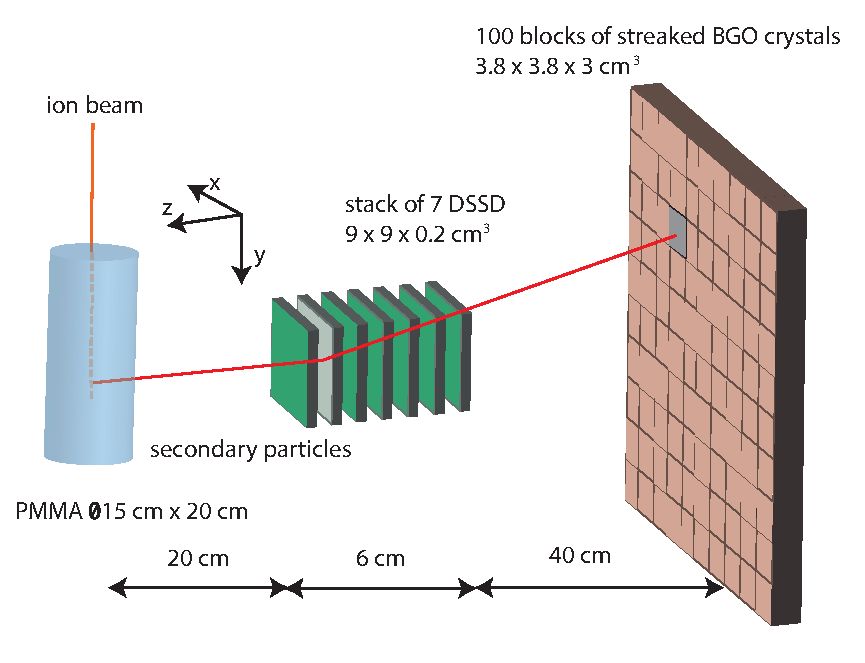
\includegraphics[width=0.7\textwidth]{./Figure/Compton_Camera_hadontherapy_PMMA_Cylinder_EN.pdf}
  \caption{Scheme of the simulation setup: a PMMA cylindrical phantom is set in front of the Compton camera prototype. The Compton camera is composed of a stack of 7 double sided silicon strip detectors (scatterer) and a plan of 100 single BGO blocks. The set distances are realistic for clinical conditions. This geometrical configuration has been used for all the simulations presented in this work.}
  \label{fig:fig_setup_CC_simulation_Hadronth}
\end{figure}

Like most of the Compton camera devices, the CLaRyS prototype includes a scatterer and an absorber. The scatterer consists of seven parallel planes of silicon detectors (double-sided silicon strip detectors, DSSDs), $9\times9\times0.2$~cm$^3$, with 1~cm distance between the centers of two neighboring planes, while the absorber is composed of an array of $10\times10$ BGO (Bismuth Germanate - Bi$_12$GeO$_20$) blocks ($3.5\times3.5\times3.0$~cm$^3$ each) placed at 40~cm from the last silicon layer (center-to-center distance). The ion beam interacts with a cylindrical PMMA (PolyMethylMethAcrylate) phantom (15~cm diameter and 20~cm length) placed in front of the Compton camera as target. It is placed 20~cm far from the first silicon plane (center-to-center distance) in order to fit with realistic clinical conditions.

The silicon detectors have a strip pitch of 1.4~mm, for a total of 64 strips per side (double-sided readout based on electron and hole pairs collection). The strips are not reproduced in the simulation code, and the transverse spatial resolution is set to 0.9~mm FWHM at the reference energy of 1~MeV, according to preliminary measurements performed on smaller detector prototypes. Concerning the parallel direction, the interaction position is set to the center of the involved silicon plane.

Regarding the BGO blocks, their entrance surface is streaked in a 8$\times$8 matrix of pseudo-pixels, 4.4~mm$^{2}$ side, and the readout is performed via 4 photo-multiplier tubes. The position reconstruction is achieved via Anger logic for the real detector, but a mono-block crystal is simulated here for simplicity. The events are selected to be limited to a single block component based on spatial analysis, and the interaction position is reconstructed via center of gravity calculation if multiple interaction occur. An incertitude contribution, randomly extracted by a Gaussian of 5~mm FWHM , is added to the reconstructed position to fit with the geometrical features. For what concerns the parallel direction, given the fact that the employed BGO blocks have not depth of interaction reconstruction capabilities, the interaction position is fixed to the center of the mono-block crystal.

Preliminary characterization measurements allowed to estimate the energy resolution of the BGO blocks, which is accordingly set to 17\% FWHM at the reference energy of 667~keV (a 137-cesium source has been used for the measurements). The energy resolution of the silicon detector is set to 2.3~keV (RMS) according to the design expectations; no characterization data are yet available for an instrumental estimate.

The time resolution has been set to 3.0~ns FWHM for the BGO blocks and to 15.0~ns FWHM for the silicon slabs, according to preliminary measurements performed on test detector modules at the GANIL %(Grand Accelerateur National d'Ions Lourds) 
center in France.

The detector resolutions play an important role in the Compton camera performances. The absorber spatial resolution influences the position of the apex of the Compton cone, as well as its axis orientation. The scatterer energy resolution determines the Compton cone aperture angle. The time resolution impacts the coincidence window between the absorber and the scatterer, and so its true/random coincidence discrimination capabilities.

The CLaRyS project also includes the development of a beam tagging hodoscope, composed of scintillating fibers read out by multi-channel photomultipliers. This detector is used to synchronize the beam time and space structure to the prompt gamma detection in order to tune the detection window reducing the background contamination. This detector section is not included in the simulation, but its time resolution has to be taken into account for the time-of-flight discrimination. It is set to 1~ns FWHM. The detectors spatial, energy and time resolutions are summarized in table \ref{table:table_resolution_detecteurs_CC_simulation_Hadronth}.

\begin{table} [!htbp]
\centering
%\begin{tabular}{>{\columncolor[gray]{0.9}}ccc}
\caption{Estimations of reachable resolutions with the detectors. Those resolutions are applied during the simulations.}
\begin{tabular}{cccc}
\hline
\textbf{Resolution (FWHM) at 1 MeV} & \textbf{Scatterer} & \textbf{Absorber} & \textbf{Hodoscope}\\
\hline 
\textbf{spatial [mm]	}			 &     0.9		 &  5 &	 1\\
%\hline
\textbf{energy}				&	2.3~keV		&  17~\%	&	/\\
%\hline
\textbf{timing [ns]}	        		&	15			&	3 	&  1\\
\hline
\end{tabular}
\label{table:table_resolution_detecteurs_CC_simulation_Hadronth}
\end{table}
    
The Monte Carlo simulation study is performed with the Geant4 toolkit, version 9.6 patch 02. Geant4 has been developed at CERN %(Conseil europ\'{e}en pour la recherche nucl\'{e}aire) 
for high energy physics experiments, but it has been shown that it can be used for ion beam therapy studies \cite{cirrone_hadrontherapy_2011,toshito_new_2010}. However, some improvements are still needed in order to extend the hadronic models to low energy applications~\cite{dedes_assessment_2014, Pinto:2016aa}.

The particle interactions in matter are described in this work by means of different models, listed in table~\ref{table:table_modele_physic_CC_simulation_Hadronth}. Additionally, the Doppler broadening and the photon polarization effects are taken into account.
 

\definecolor{Gray}{gray}{0.9}

\begin{table}[ht]
\label{physlist_ion}
\caption{Hadronic models used in the Geant4 simulations.}
\begin{scriptsize}
\begin{center}
\renewcommand{\arraystretch}{1.2}
%\begin{tabular} {>{\columncolor[gray]{0.9}}cccc}\hline  
\begin{tabular} {cccc}\hline
%\rowcolor{Gray}
\textbf{Process} & \textbf{Protons} & \textbf{Ions} & \textbf{Neutrons} \\ \hline 
\textbf{Electromagnetic} & \multicolumn{3}{c}{standard$_{\rm{option3}}$} \\ %\hline
\textbf{Inelastic} & G4BinaryCascade & G4QMDReaction  &  G4BinaryCascade  \\ 
 & & (G4IonsShenCrossSection)&+ G4NeutronHPInelastic ($<$19 MeV)\\ %\hline
\textbf{Elastic} & G4LElastic & G4LElastic & G4LElastic + G4NeutronHPElastic ($<$19 MeV)\\ %\hline
\textbf{Fission} & / & / & G4LFission + G4NeutronHPFission($<$19 MeV) \\ %\hline
\textbf{Capture} & / & / & G4LCapture +  G4NeutronHPCapture ($<$19 MeV) \\ %\hline
\textbf{Radioactivedecay} & / & G4Radioactivedecay & / \\ \hline
\end{tabular}
\end{center}
\end{scriptsize}
\label{table:table_modele_physic_CC_simulation_Hadronth}
\end{table}

The two main beam particles used in clinics are considered in this work: protons and carbon ions. The beam range of interest is 15.2~cm in the PMMA phantom, and the associated energy is 160~MeV for protons and 305~MeV/n for carbon ions.
 
In order to reproduce a realistic clinical beam, the beam transverse dimension is modeled with a Gaussian distribution with a standard deviation of 5~mm for protons at 160~MeV and 3.5~mm for carbon ions at 305~MeV/n. The Compton camera setup does not change for the different incident particles. The beam intensity for a spot in pencil beam scanning (PBS) mode for protons is $10^8$~particles and $10^5$~particles for carbon ions. The beam time structure is applied in the data analysis stage, described below.\newline

\subsection{Data treatment}
\label{subsection:Treatment_data_CC_hadrontherapy_Geant4}

\subsubsection{Time structure and treatment}
\label{subsubsection:modelisation_fasceau_ions_CC_hadrontherapy_Geant4}
 
Two different beam time structures have been considered for this study, related to two kinds of accelerators used in clinical practice: the IBA C230 cyclotron for protons (used in 16 clinical centers worldwide) and the Heidelberg (Germany) synchrotron installed in the Ion Therapy Center (HIT) for carbon ions. Even if the beam microstructure changes depending on the ion energy and the beam intensity, the microstructure is modeled according to the reported features at a specific energy and intensity for simplicity. For protons at 160 MeV, the primary particles are grouped in bunches of 2~ns (this value may vary also according to the distance between the cyclotron and the treatment room, and energy spread selection) at a frequency of 106~MHz (9.42~ns)~\cite{f_roellinghoff_real-time_2014}. The clinical beam intensity is 3.2~nA which corresponds to about 200 protons per bunch. Concerning the carbon ion beam at 305~MeV/u, the estimated microstructure is composed of 30~ns duration bunches at a frequency of 5.9~MHz (170~ns period). The clinical beam intensity for carbon ions is $5\times10^7$~ions/s, corresponding to about 9~ions per bunch. This beam structure is extrapolated from measurements performed by our group in 2013 at HIT; the beam time structure was measured for 200~MeV/u and 400~MeV/u primary ion energy with a two-fiber hodoscope (basic prototype of the one at present under development) and the spill signal was given by the accelerator. Figure \ref{fig:fig_structure_temps_faisceau_HIT_2013_CC_simulation_Hadronth} shows the beam structure for carbon ions at 400~MeV/u. The pulses have a spill period of 150.2~ns and each bunch is approximately 21.5~ns.
The mentioned measurements have shown that the spill phase changes during the extraction: this implies that the HF signal from the synchrotron can not be used to trigger the pulses, so that the use of an additional beam time stamp system like the hodoscope seems required for time-of-flight background rejection purposes.\newline

	\begin{figure} [!hbtp]	
	\centering
	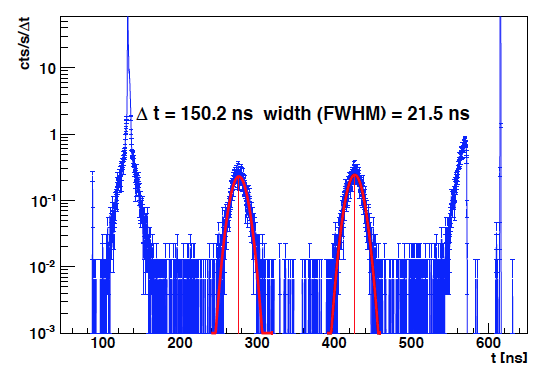
\includegraphics[width=0.5\textwidth]{./Figure/2013_Structure_Time_Beam_400MeV.png}
	\caption{Time micro-structure measured from a carbon ion beam at 400~MeV/u delivered at HIT. The pulses have an extraction period of 150.2~ns and the bunches are 21.5~ns FWHM. The measurement was achieved with a two-scintillating-fiber hodoscope.}
	\label{fig:fig_structure_temps_faisceau_HIT_2013_CC_simulation_Hadronth}
	\end{figure}


The coincidence window (between scatterer and absorber events) is set to 40~ns, centered on each absorber detected interaction. This value is adapted to the detectors time resolutions. Table~\ref{table:definition_beam_structure_CC_hadrontherapy_Geant4} summarizes the presented beam time structures and coincidence reconstruction features.

\begin{table} [!htbp]
\footnotesize
\centering
\caption{Description of the two beam structures studied: the IBA cyclotron C230 for protons and the synchrotron installed at the Heidelberg Ion Therapy Center (HIT) in Germany for carbon ions. The macro-structure of the synchrotron, at the second time scale, is not considered here. The beam structures are applied to the simulation data.}
\setlength{\tabcolsep}{2pt}
%\hspace{-2.1cm}
\begin{tabular}{c>{\columncolor[gray]{0.9}}ccc}
\cline{2-4}
%\hline
		\multicolumn{2}{c}{ }		 & 					\textbf{Protons} & \textbf{Carbon ions}\\ 
%\hline
\cline{2-4}%\hline
\multirow{3}{*}\textbf{Clinical features}		&	\textbf{Facility}	& IBA Cyclotron C230&   Synchrotron at HIT\\
											& \textbf{Clinical intensity}& $  2\times10^{10}$ p/s  & $  5\times10^{7}$ ions/s\\
											& \textbf{Energy} 			&160 MeV 			&    305 MeV/u\\
\cline{2-4}%\hline
\multirow{3}{*}\textbf{Beam structure}		&	\textbf{Bunch time [ns]}			& 3.2				&  30\\
											& \textbf{Period [ns]}		&   9.4 				& 170\\
											& \textbf{Primaries  /bunch} 	&217 			& 9\\
\cline{2-4}%\hline
\multirow{2}{*}\textbf{Detectors}						& \textbf{Coincidence window [ns]}		& 40 	&  40 \\
											&\textbf{Time resolution [ns]} & \multicolumn{2}{c}{Si: 15 and BGO: 3}\\
\cline{2-4}%\hline
\end{tabular}
\label{table:definition_beam_structure_CC_hadrontherapy_Geant4}
\end{table}



\newpage
%---------------------------------------------------------------
%---------------------------------------------------------------
\subsubsection{Data selection: time and energy cuts}
\label{MatMeth::TOF_Ecut}

As already explained in the introduction, the Compton detection principle is based on a double interaction in the scatterer and absorber section, where an interaction is defined as an energy deposit in a detector module. As discussed in section~\ref{subsubsection:modelisation_fasceau_ions_CC_hadrontherapy_Geant4}, the coincidence reconstruction relies on a defined time window, fixed according to the involved detector resolution. In a simulation environment, different kinds of coincidences events can be distinguished and studied: 
\begin{itemize}
\item[-] real coincidences: created by a single photon first interaction in a single scatterer plane and then in a single absorber block;
\item[-] quasi-simultaneous interaction from two secondary particles;
\item[-] double interaction from the same particle different from a gamma.
\end{itemize}

In a real clinical environment there is no way to select the real coincidences, so that the collected data are affected by a certain number of the so-called random coincidences. The amount of random coincidences depends on the detector time resolutions, on the fixed time coincidence window and on the beam time structure, for fixed beam energy, phantom composition and camera prototype setup. In figure~\ref{fig:fig_explication_coincidence_CC_simulation_Hadronth} a schematic view of the different kinds of coincidences is presented.

\begin{figure} [!hbtp]	
  \centering
  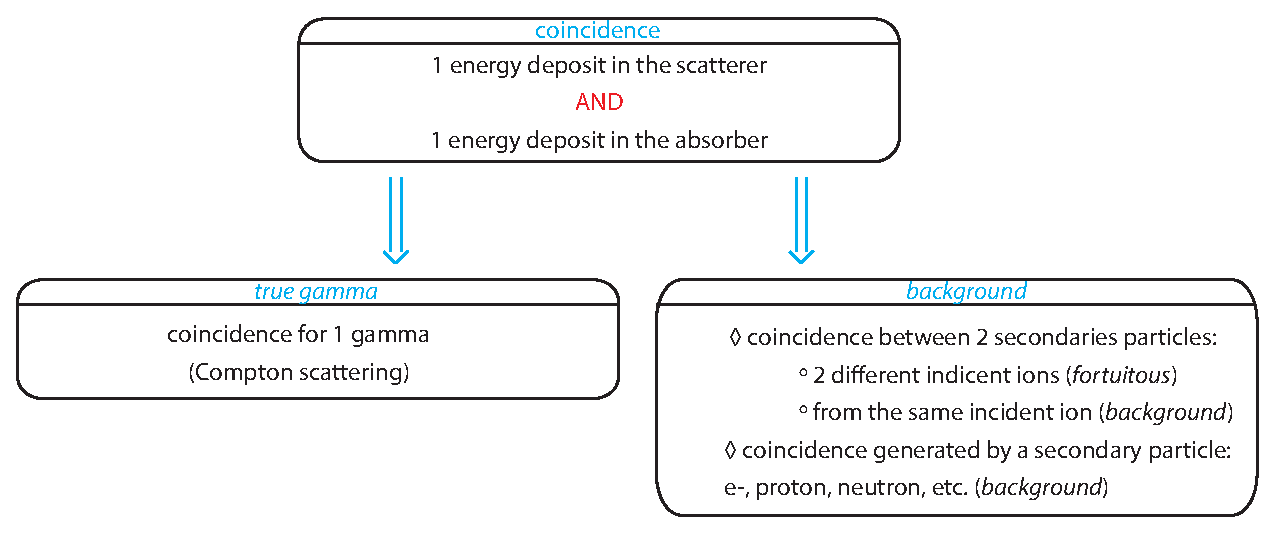
\includegraphics[width=0.9\textwidth]{./Figure/Schema_coincidence_EN.eps}
  \caption{Diagram showing the different definitions of coincidences in the Compton camera.}
  \label{fig:fig_explication_coincidence_CC_simulation_Hadronth}
\end{figure}

In addition to this, the prompt gamma measurement is contaminated by other secondary particles produced by the beam interaction with the patient/phantom, mainly massive and charged particles (protons, neutrons). 
As already mentioned, it has been demonstrated by our group that a time-of-flight discrimination is possible and effective in reducing this source of background. In fact, the photons are moving at the speed of light while the massive particles approach the detector at a lowest speed. The time information coming from the hodoscope and from the absorber can be then combined to fix a detection time window and reject all the events outside the window. In this work, the time between the incident particle creation and the secondary particle detection in the absorber is considered as the time-of-flight. The hodoscope time resolution $u_{hodoscope}$ (1~ns FWHM) is applied to the primary particle creation time, with a contribution randomly extracted from a Gaussian with $\sigma\,=$ 1/2.35~ns, while the detection time in the absorber is affected by the absorber time resolution.

 \begin{eqnarray}
TOF_{theoretical} = t_{absorber}-t_{hodoscope} \\
TOF_{simulation} = t_{absorber}+t_{creation} + u_{hodoscope}
\label{TOF_equation}
\end{eqnarray} 

The time-of-flight spectrum resulting from the simulation shows that the coincidences of interest (produced by prompt-gamma rays) are included in a window between 0 and 6~ns (figure \ref{fig:fig_TOF_distribution_CC_simulation_Hadronth}). Therefore, all the coincidences with a TOF higher than 6~ns have been rejected, reproducing a possible clinical background rejection scenario. 

\begin{figure} [!hbtp]	
  \centering
  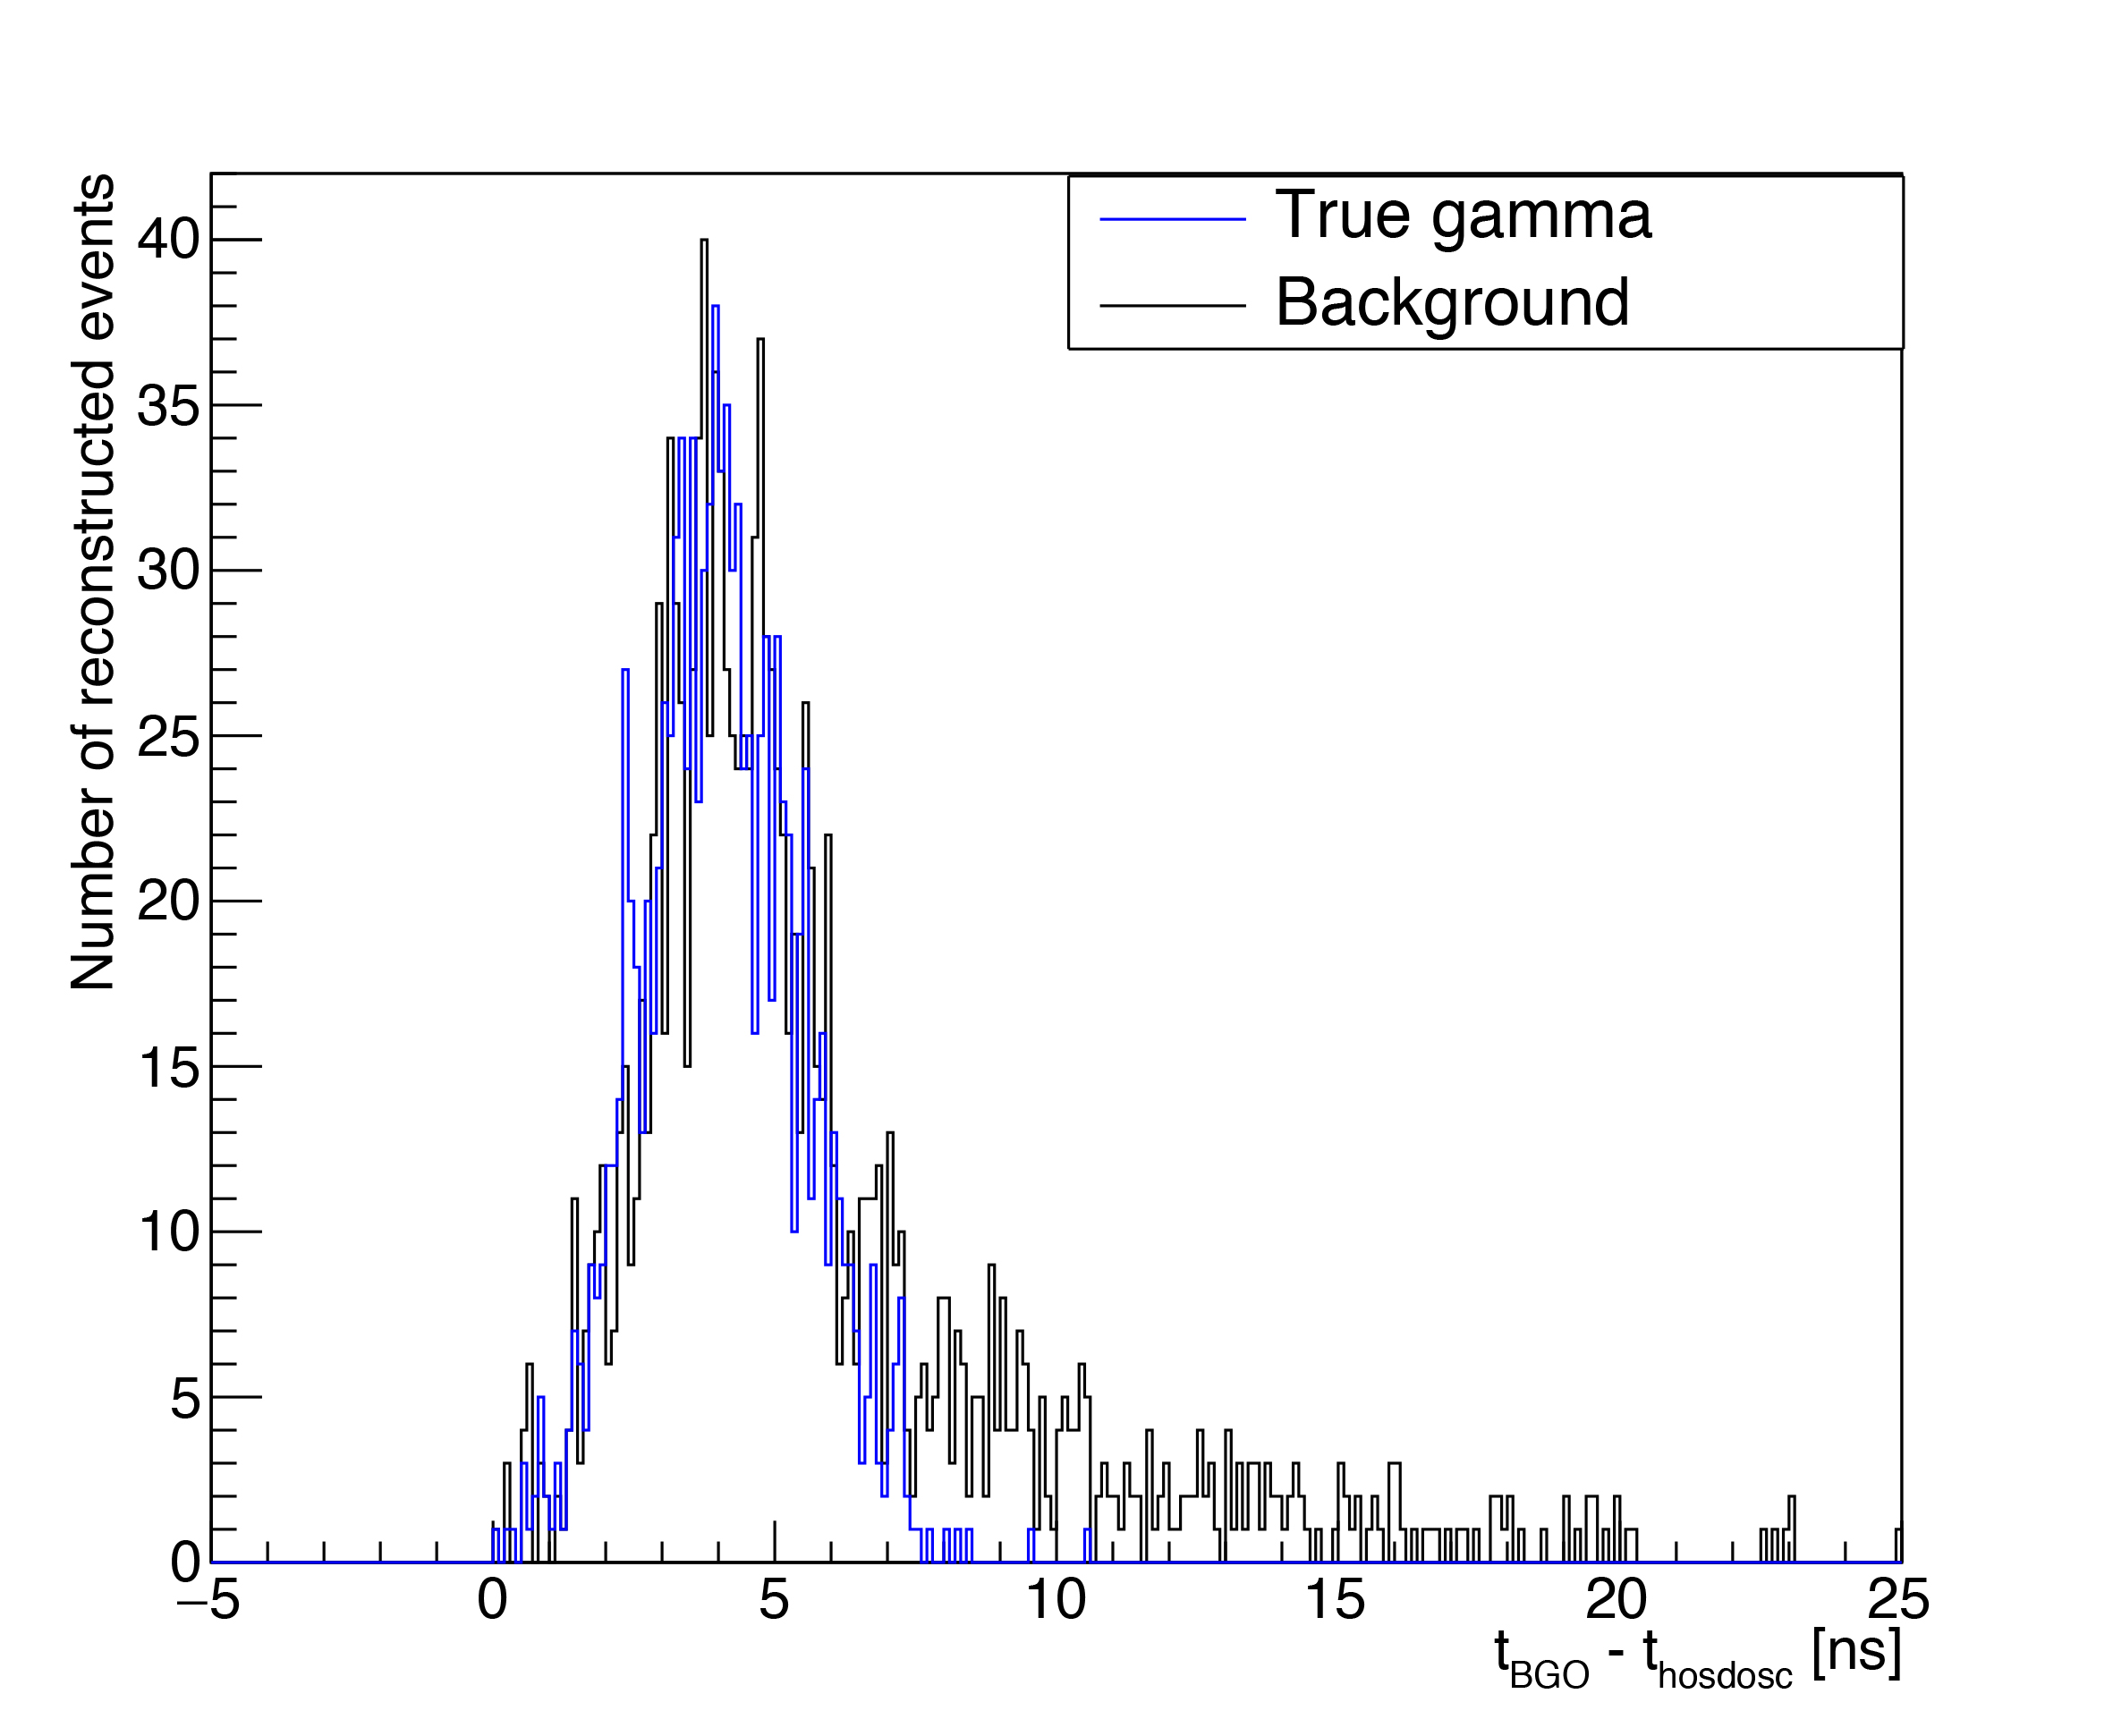
\includegraphics[width=0.6\textwidth]{./Figure/2015_01_04_TOF_spectra_NoCut_1Proton_ResolTemporelle_applied_these.jpg}
  \caption{Time of flight spectrum obtained by means of the simulation for a proton beam at 160 MeV and $1\times10^{8}$ incident protons. The detection time for the absorber is given by the tag for the first deposit energy. The blue curve represents the time of flight for true events and the black one represents the background.}	
  \label{fig:fig_TOF_distribution_CC_simulation_Hadronth}
\end{figure}

In addition to the time-of-flight based selection, energy thresholds are also defined for the event detection. On a single detector basis, 50~keV is set as lower threshold for the silicon layers and 100~keV for the absorber. On a complete event basis, a total absorbed energy lower limit is set to 1~MeV.

\subsection{Reconstruction algorithm}

Once the coincidences are defined and selected according to the fixed physical cuts, the prompt-gamma emission point has to be reconstructed for each event. This can be done via analytic or iterative algorithms based on the Compton kinematics (see section~\ref{section::Intro}), presented in the following sections.


\subsubsection{Line-cone algorithm}
The reconstruction via line-cone algorithm exploits the energy deposit and position information collected by the camera in addition to the beam path information. Thanks to the deposited energies in the detectors and the interaction positions, a cone surface is analytically defined via the Compton equation~\ref{Compton_equation}.
\newline
We assume that the initial energy of the gamma ray is fully absorbed in the absorber. This hypothesis, combined to the detector energy resolutions, leads to a potential uncertainty on the cone aperture. The interaction position in the scatter gives the cone apex and the line connecting the interaction position in scatterer and absorber gives the cone axis. In order to simplify the reconstruction, the beam direction is used to limit the possible solutions (laying on the reconstructed cone surface) to two points (intersection of the beam direction and the reconstructed cone). The set of all the reconstructed points gives the emission source distribution. The obtained final image is then the 2 dimensional projection of the prompt gamma emission spectrum. 

\subsubsection{LM-MLEM algorithm}	

The iterative methods allow to get a 3D image reconstruction, potentially by taking into account the spatial resolution and the energy resolution of the detectors. Few iterative algorithms have been developed for Compton event reconstruction. \cite{schone_common_2010, zoglauer_design_2011,gillam_compton_2011,mackin_evaluation_2012,lojacono_low_2013}.

The \textit{List-Mode Maximum Likelihood Expectation Maximization} (LM-MLEM) algorithm is a MLEM version which allows to free from sinograms and to reconstruct the image directly from the list of detected events.
The first step is to define the volume which includes the origin of the prompt gamma ray detected. This volume is divided into equal voxels and the emission intensity is assumed homogeneous for each voxel $j$, with a Poisson distribution of parameter $\lambda_j$ (a vector of the emissions intensities of all the voxels). The algorithm is based on a system matrix $T$ composed of the coefficients  $t_{ij}$ which represent the probability that a photon produced in the voxel $j$ is detected in coincidence by the Compton camera as an event $i$. The probability for a gamma detected in coincidence to be emitted from the voxel $j$ is denoted as $s_j$.
The LM-MLEM algorithm starts with an initial value $\lambda^{(0)}$, which can be the simple back-projection reconstruction.
The iterations rely on the following recurrence relation:

\begin{equation}
\lambda_j^{(l+1)} =  \frac{\lambda_j^{(l)} }{s_j} \sum\limits_{i=1}^{N_{\gamma}} t_{ij} \frac{1}{P_i^{(l)}},\quad \rm{with}\quad  P_i^{(l)}=\sum\limits_{k=1}^{N_{v}} t_{ij}\lambda_k^{(l)},
 \label{eq:equation_lambda_compton_med_nucleaire}\newline
\end{equation}
where $N_{\gamma}$ is the number of detected events and $N_v$ is the number of voxels in the image.\newline

The LM-MLEM algorithm used for this study is the one developed by the CREATIS research group in Lyon~\cite{maxim_filtered_2014,hilaire_compton_2014}.\newline%\cite{maxim_analytical_2009,lojacono_low_2013,maxim_filtered_2014,hilaire_compton_2014}.\newline
For each photon detected, the system matrix $T$ is calculated by taking into account the uncertainties on the angle between the source and the involved scatterer plane and the angle between the scatterer plane and the absorber involved module.
The matrix elements $t_{ij}$ are calculated as:
\begin{equation}
 t_{ij} = K(\beta_i,E_{tot})\frac{|\rm{cos}(\theta_{\overrightarrow{V2V1})} |}{V_2V_1^2} \int\limits_{M\in v_j} \frac{|\rm{cos}(\theta_{\overrightarrow{V_1M})}| }{V_1M^2} h_i(M)dv,
 \label{eq:equation_tij_compton_med_nucleaire}\newline
\end{equation}
where $\beta_i$ is the Compton scattering angle, $V_1$ the interaction position in the scatterer, $V_2$ the interaction position in the absorber, $h_i$ the spatial kernel which models the uncertainties on the Compton angle for each voxel $M$, $K(\beta_i,E_{tot})$ the differential cross section and $v$ the reconstructed volume.\newline

In order to simplify and speed up the calculation of the $t_{ij}$ matrix, the voxels located far from the reconstructed cone are set to 0. The distance between the cone and the voxel is calculated by taking the voxel center as reference point. The spatial resolutions are not included in this version of the algorithm.\newline
For each iteration, the matrix $T$ is stored and the reconstructed image can be produced via a Matlab simple interface.

\subsection{Precision estimation}

The camera precision is defined as the difference between the expected Bragg peak position (according to the treatment planning) and the Bragg peak position reconstructed through the data. This is a critical parameter which will be used to fix a decision threshold during a ion beam treatment.
 
In this study a reference profile has been defined as the reconstructed emission vertex profile at high statistics, via analytic (line cone) and iterative (LM-MLEM) algorithms; this will be used to mimic the treatment planning. This Bragg peak position is compared to the ones reconstructed at lower statistics (close to clinical conditions) via analytic and iterative algorithms.

The high statistic profile has been obtained with $2\times10^{10}$ incident protons (figure~\ref{fig:fig_Results_Estimation_Camera_Profil_highStat_CC_simulation_Hadronth_LineCone}) for the line-cone reconstruction and with $1\times10^{10}$ incident protons (figure~\ref{fig:fig_Results_Estimation_Camera_Profil_highStat_CC_simulation_Hadronth_MLEM}) for the LM-MLEM reconstruction method. The \textit{SmoothKern} method, with the Nadaraya-Watson regression, is used to smooth the reference profiles in order to reduce relative statistic fluctuations.\newline
A region of interest (ROI) ranging from $y=0$ mm to $y=+100$ mm is defined around the expected Bragg peak position, located at $y=+50$~mm in the phantom. The reference profiles are modelled in the ROI by a linear combination named Non-Uniform Rational Basis Splines (NURBS). \newline
A new independent profile should be simulated at low statistics for the precision calculation. However, with the aim to speed up the analysis, a random extraction from the NURBS profile (\ref {fig:fig_Estimation_Camera_CC_NURBS_Poisson_LC} and \ref {fig:fig_Estimation_Camera_CC_NURBS_Poisson_MLEM}) is performed following the Poisson law, in order to select reduced data sets. The desired low statistics ranges from $10^8$ to $5\times10^9$ incident protons.\newline
The minimal distance between the NURBS reference profile and the low statistic reconstructed profiles is estimated thanks to the $\chi^2$ method. For the $\chi^2$ estimate, the low statistics profile is defined around the fall-off position from $y=+30$ mm to $y=+70$ mm. The minimization process tests the profiles at low statistics on a 60 mm variation range, between $-30$~mm and $+30$~mm with respect to the initial position, with a step of $0.1$~mm. The      $\chi^2$ is calculated as follows:

\begin{eqnarray}
\chi^2 = \sum\limits_{i=1} {(y_{sample,i}-y_{NURBS,i})^2},
\end{eqnarray}

where $y_{sample}$ is the number of coincidences for the low statistics profile, $y_{NURBS}$ is the number of coincidences for the reference profile NURBS (scaled at the same low statistic) and i the step number.\newline
The global minimum of all the reconstructed profiles is then retrieved. The figures \ref{fig:fig_Results_Chi2_Distribution_Variation_CC_simulation_Hadronth_LC} and  \ref{fig:fig_Results_Chi2_Distribution_Variation_CC_simulation_Hadronth_MLEM} show the distribution of $\chi^2$ calculated for a low statistic profile at $10^8$ incident protons.\newline
A total of a thousand profiles at the low statistic are generated (named realizations) and the $\chi^2$ minimization is applied to each of them. The standard deviation of the distribution resulting of the thousand results gives the precision of the camera for a given number of incident protons. The figure~\ref{fig:fig_Results_Precision_Distribution_Variation_CC_simulation_Hadronth_LC} and~\ref{fig:fig_Results_Precision_Distribution_Variation_CC_simulation_Hadronth_MLEM} show the distributions at $10^8$ incident protons for the line-cone and LM-MLEM algorithms.


\begin{figure} [!h]
\subfloat[\label{fig:fig_Results_Estimation_Camera_Profil_highStat_CC_simulation_Hadronth_LineCone}]{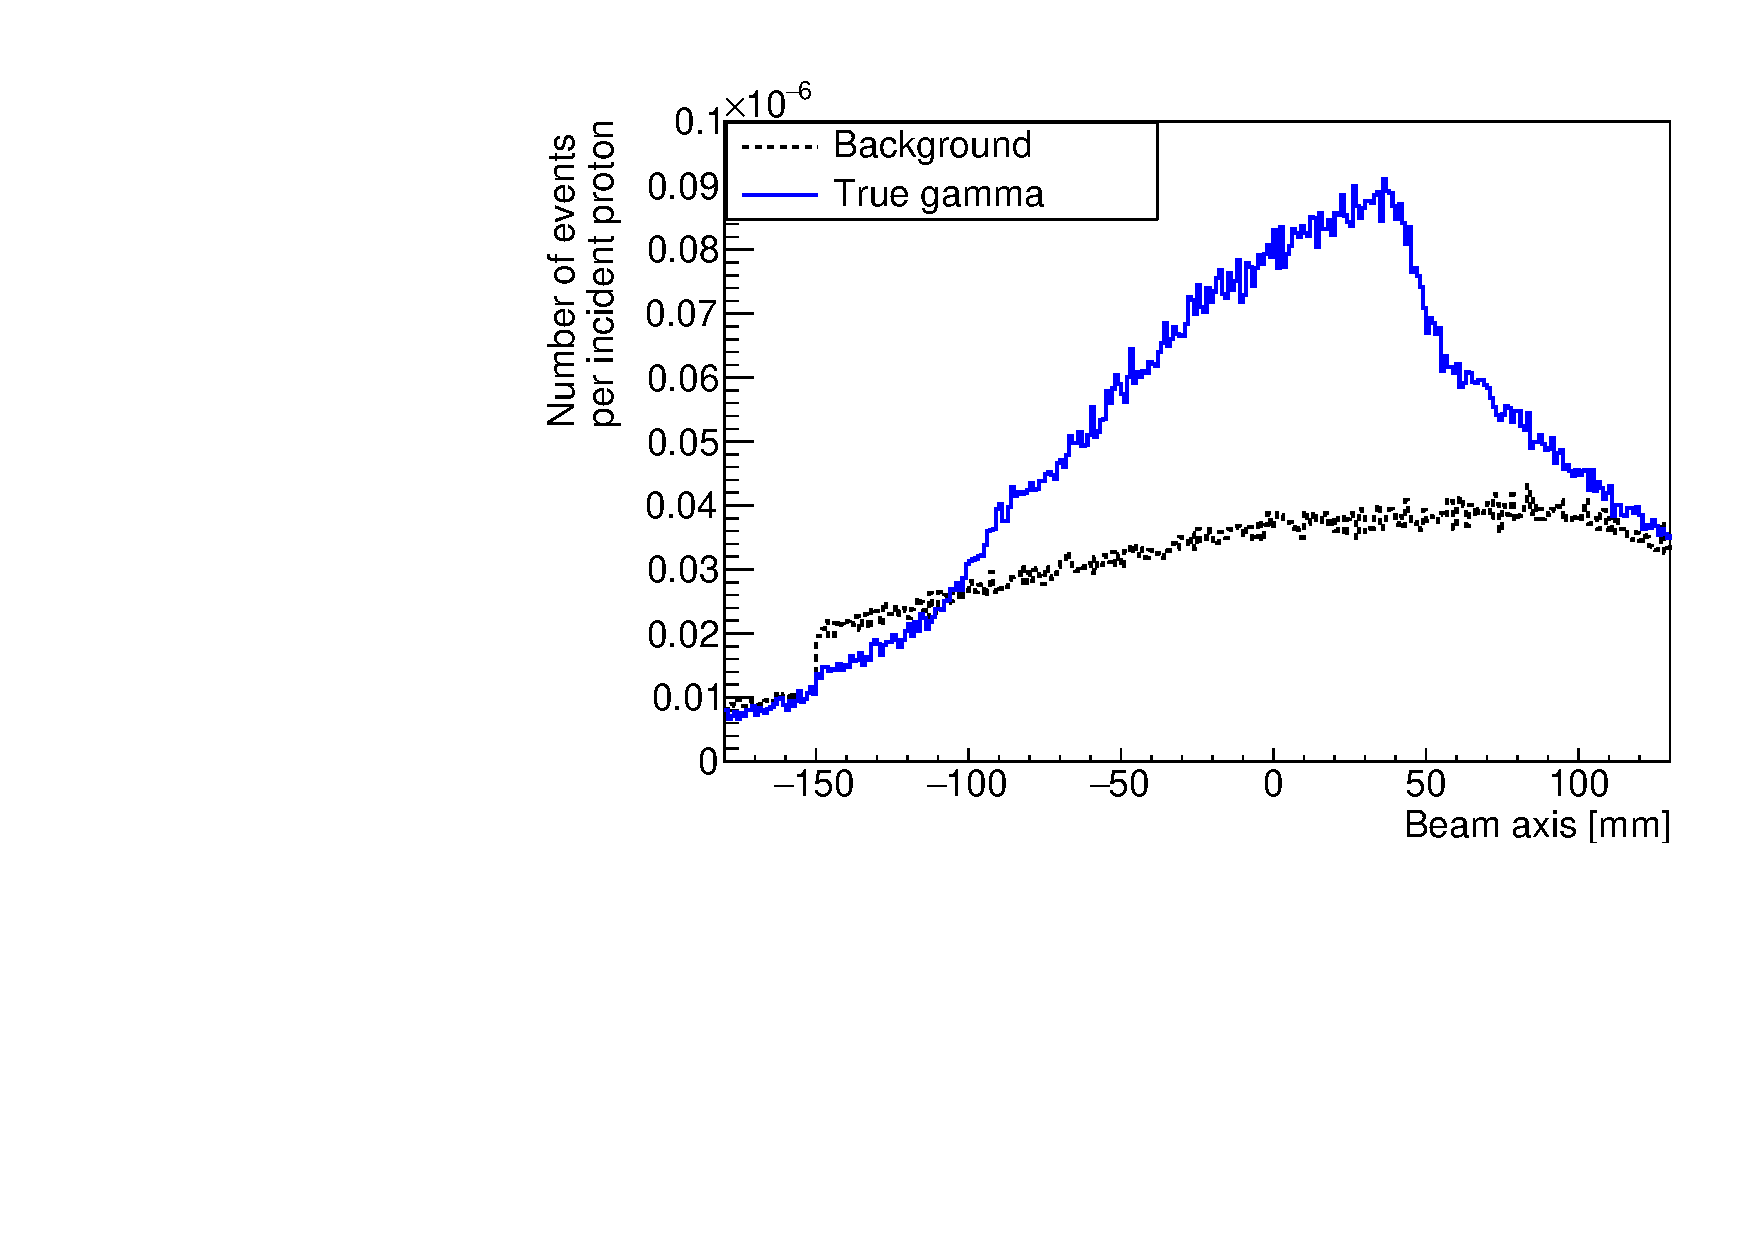
\includegraphics[width=0.33\textwidth]{./Figure/2015_04_10_Profil_Reconstruction_ligne_cone_centre_pic_de_bragg_stat_26e9.pdf}}
 \subfloat[\label{fig:fig_Results_Estimation_Camera_Profil_highStat_CC_simulation_Hadronth_MLEM}]{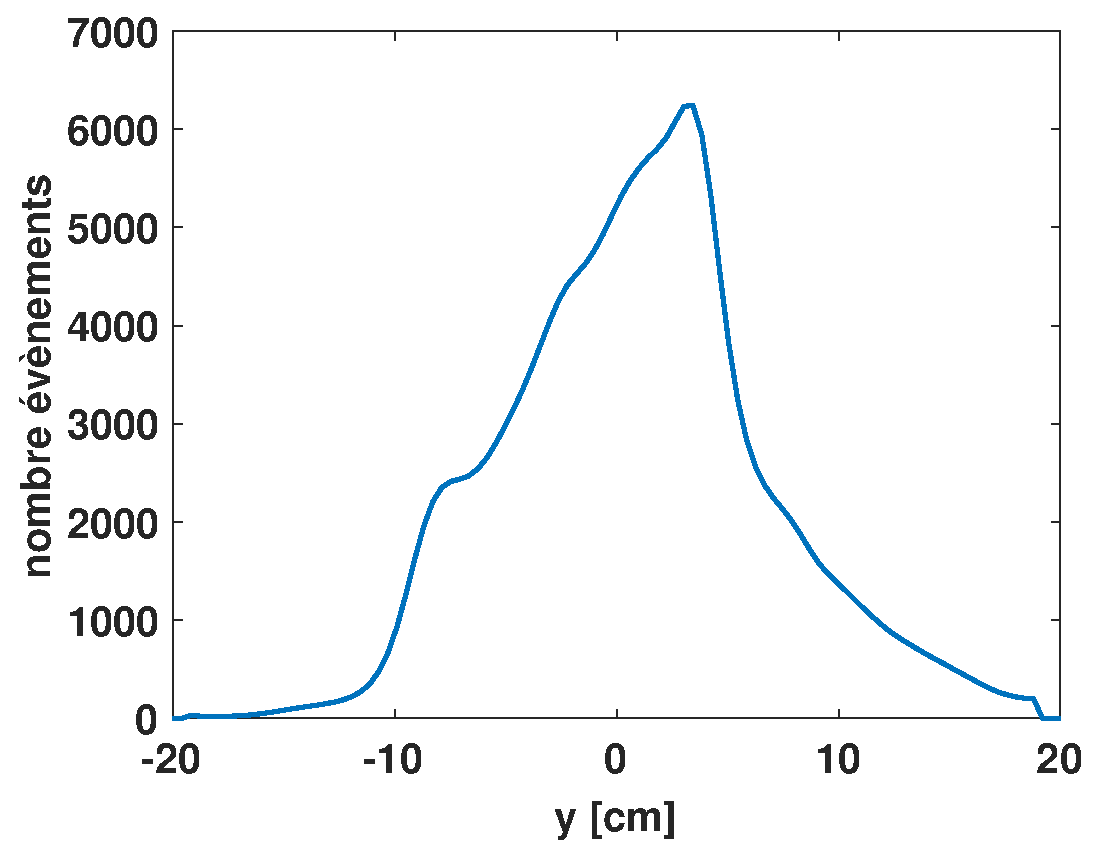
\includegraphics[width=0.33\textwidth]{./Figure/MLEM.eps}}\\
 \subfloat[\label{fig:fig_Estimation_Camera_CC_NURBS_Poisson_LC}]{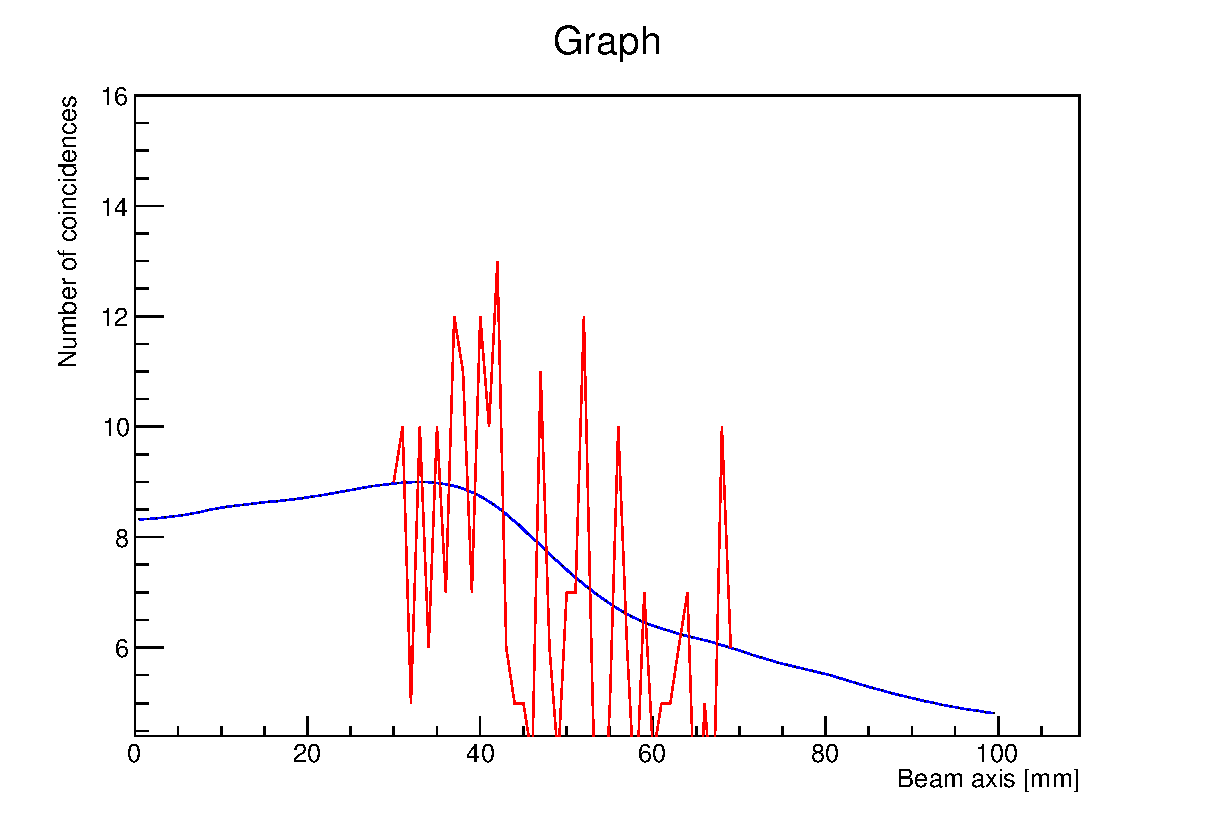
\includegraphics[width=0.33\textwidth]{./Figure/2017-08-02_Poisson_Nurbs_1e8_Article_LC.eps}}
 \subfloat[\label{fig:fig_Estimation_Camera_CC_NURBS_Poisson_MLEM}]{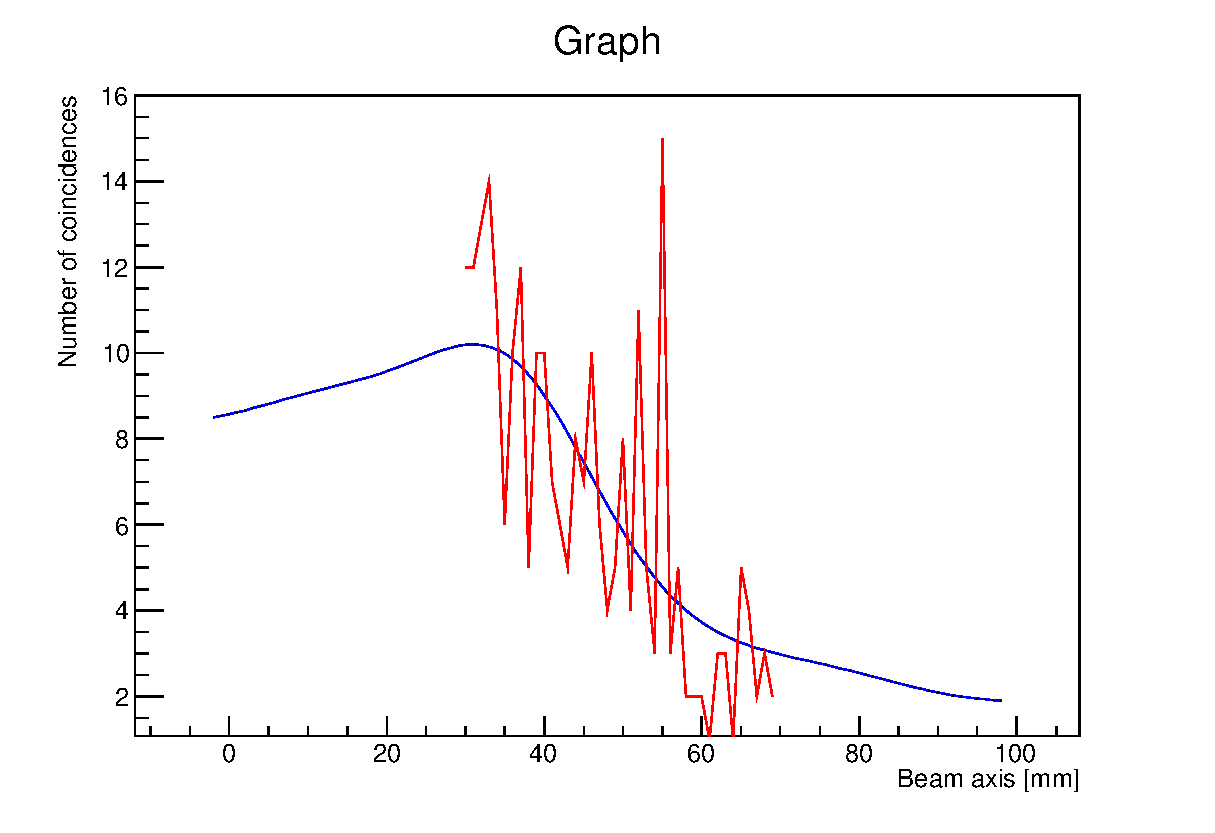
\includegraphics[width=0.33\textwidth]{./Figure/2017-08-02_Nurbs_Poisson_1e8_Article_MLEM.eps}}\\
  \subfloat[\label{fig:fig_Results_Chi2_Distribution_Variation_CC_simulation_Hadronth_LC}]{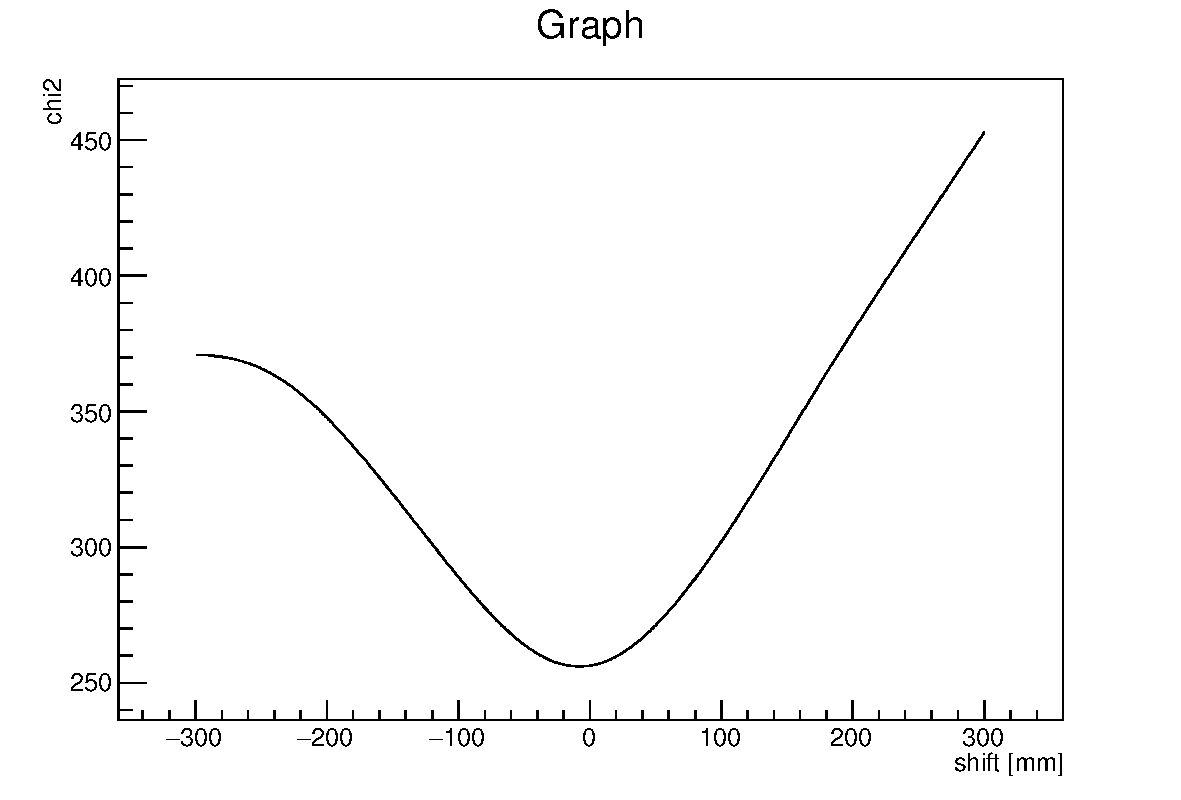
\includegraphics[width=0.33\textwidth]{./Figure/2017-08-02_Distribution_Chi2_1e8_LC.pdf}}
 \subfloat[\label{fig:fig_Results_Chi2_Distribution_Variation_CC_simulation_Hadronth_MLEM}]{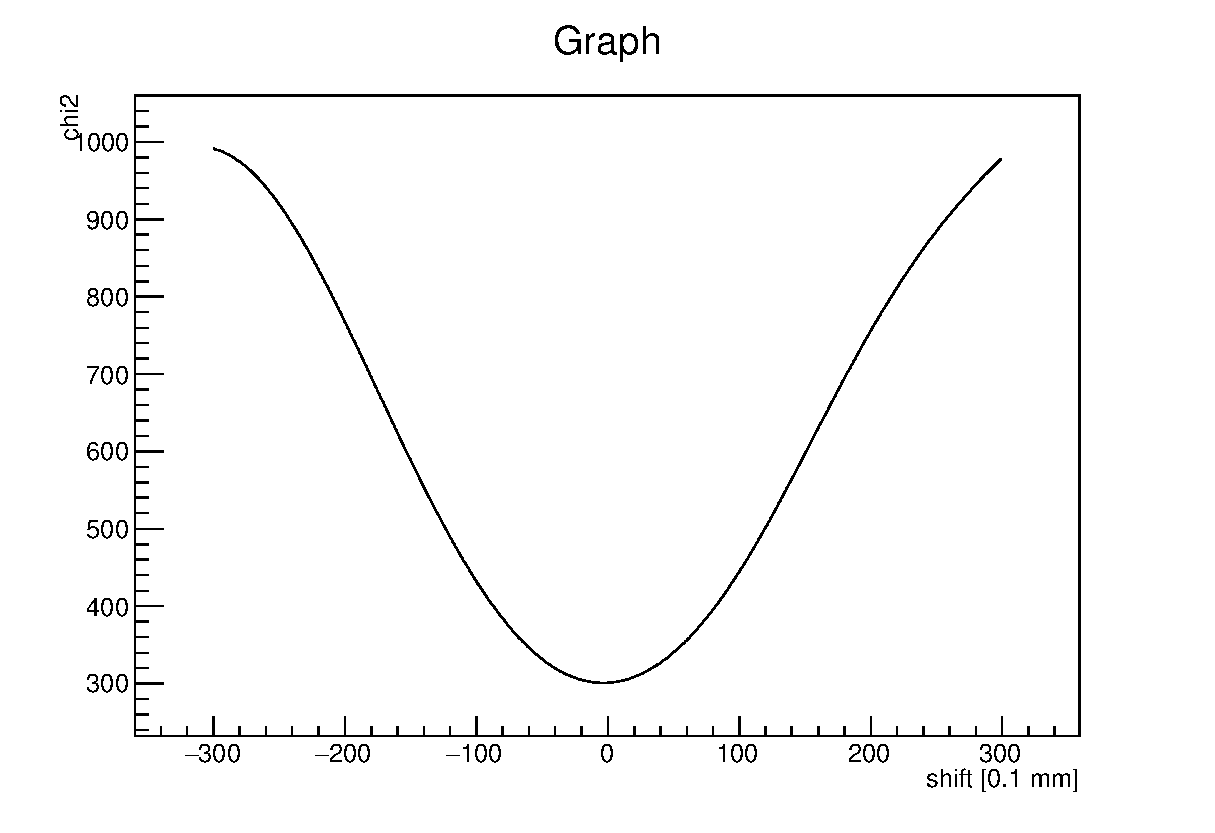
\includegraphics[width=0.33\textwidth]{./Figure/2017-08-02_Distribution_Chi2_Results_binning_1mm_ShiftNurbs0_1mm_1e8_article_MLEM.eps}}\\
  \subfloat[\label{fig:fig_Results_Precision_Distribution_Variation_CC_simulation_Hadronth_LC} ]{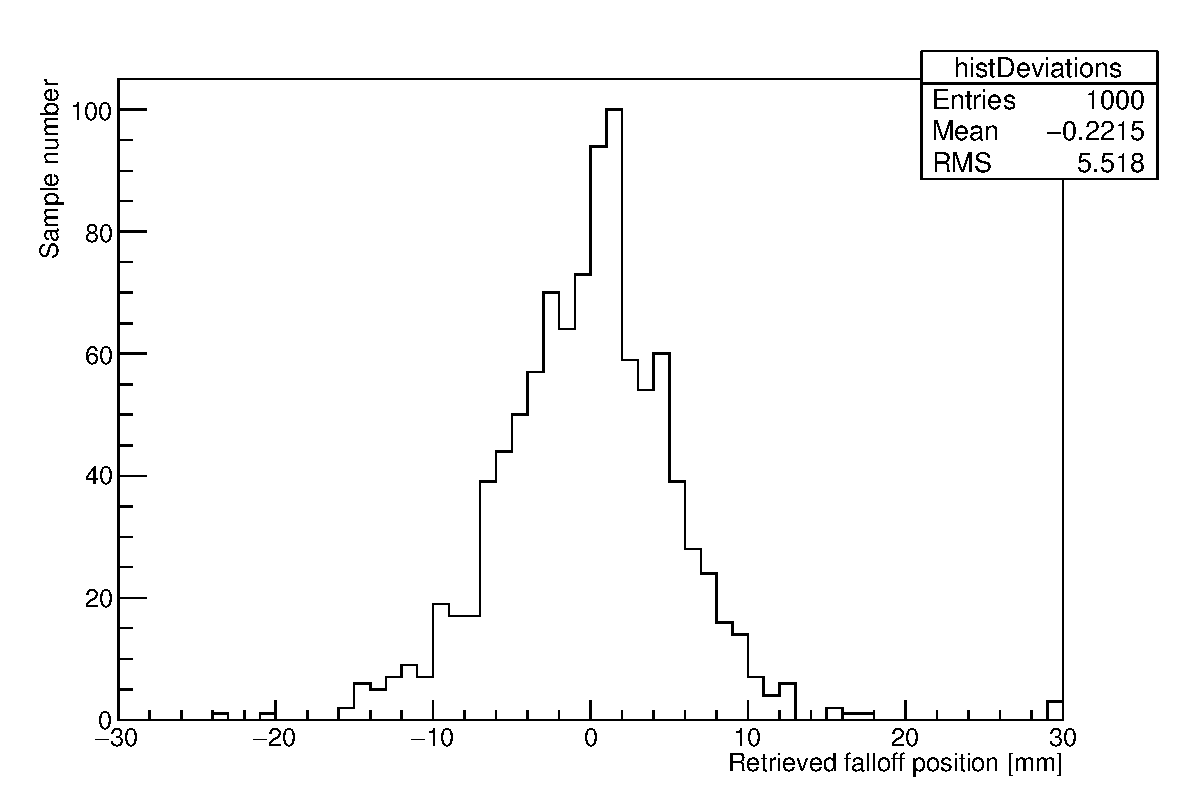
\includegraphics[width=0.33\textwidth]{./Figure/2017-08-02_Distribution_finale_1e8_Article_LC.pdf}}
 \subfloat[\label{fig:fig_Results_Precision_Distribution_Variation_CC_simulation_Hadronth_MLEM} ]{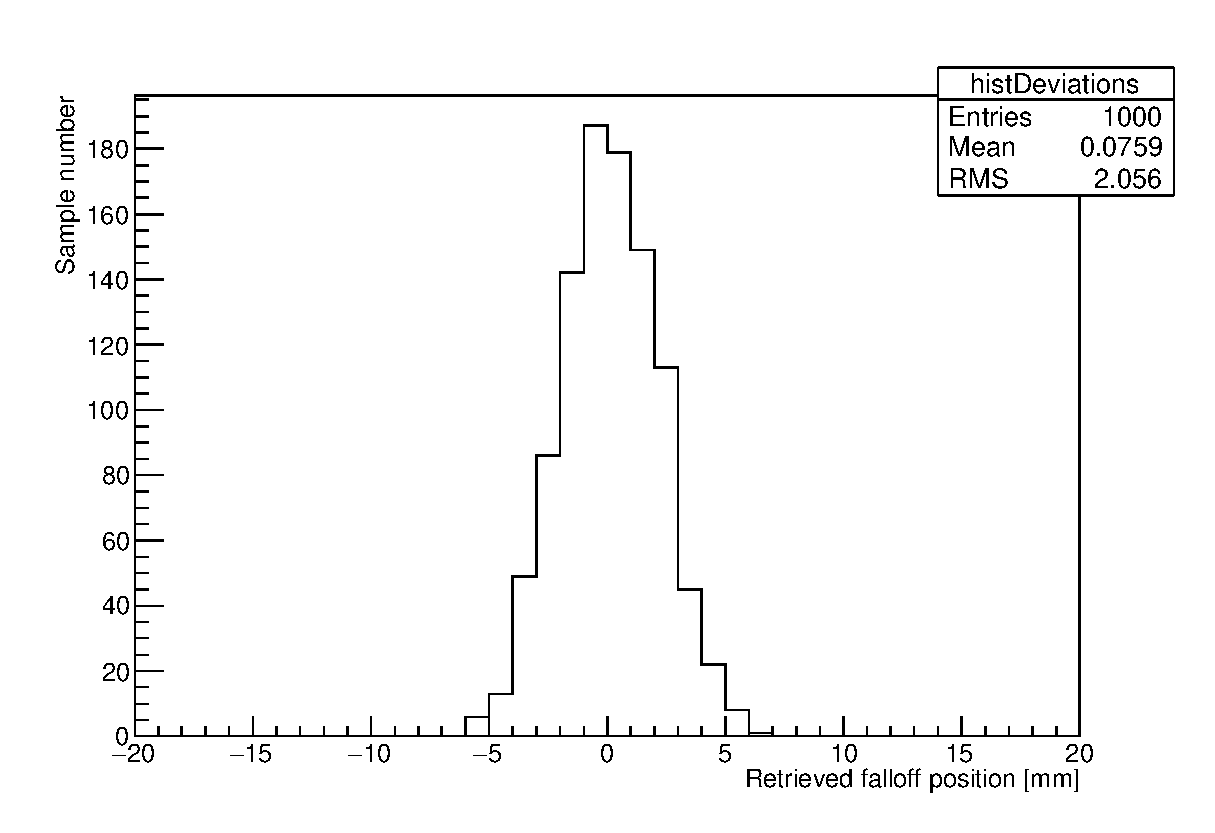
\includegraphics[width=0.33\textwidth]{./Figure/2017-08-02_FallOff_Results_binning_1mm_ShiftNurbs0_1mm_1e8_Article_MLEM.eps}}
\caption{Treatment comparison for the same proton simulation with the line cone algorithm (left column: figures \ref{fig:fig_Results_Estimation_Camera_Profil_highStat_CC_simulation_Hadronth_LineCone}, \ref{fig:fig_Estimation_Camera_CC_NURBS_Poisson_LC}, \ref{fig:fig_Results_Chi2_Distribution_Variation_CC_simulation_Hadronth_LC}, \ref{fig:fig_Results_Precision_Distribution_Variation_CC_simulation_Hadronth_LC}) and the LM-MLEM algorithm (right column: figures \ref{fig:fig_Results_Estimation_Camera_Profil_highStat_CC_simulation_Hadronth_MLEM}, \ref{fig:fig_Estimation_Camera_CC_NURBS_Poisson_MLEM}, \ref{fig:fig_Results_Chi2_Distribution_Variation_CC_simulation_Hadronth_MLEM}, \ref{fig:fig_Results_Precision_Distribution_Variation_CC_simulation_Hadronth_MLEM}). The first row gives the reconstructed profile for $2\times10^{10}$ incident protons (figure \ref{fig:fig_Results_Estimation_Camera_Profil_highStat_CC_simulation_Hadronth_LineCone}) and for $1\times10^{10}$ incident protons (figure \ref{fig:fig_Results_Estimation_Camera_Profil_highStat_CC_simulation_Hadronth_MLEM}) respectively. The figures \ref{fig:fig_Estimation_Camera_CC_NURBS_Poisson_LC} and \ref{fig:fig_Estimation_Camera_CC_NURBS_Poisson_MLEM} are showing the reference curve (blue) and the estimated curve with Poisson's law at $1\times10^8$ incident protons. The figures \ref{fig:fig_Results_Chi2_Distribution_Variation_CC_simulation_Hadronth_LC} and \ref{fig:fig_Results_Chi2_Distribution_Variation_CC_simulation_Hadronth_MLEM} are the $\chi^2$ minimization results for one realization. The minimum of the curve gives the best fit between the reference curve and the low statistics one. Finally, the figures  \ref{fig:fig_Results_Precision_Distribution_Variation_CC_simulation_Hadronth_LC} and \ref{fig:fig_Results_Precision_Distribution_Variation_CC_simulation_Hadronth_MLEM} represents the results for 1000 $\chi^2$ minimizations. The Compton camera precision is estimated thanks to the standard deviation of the distribution. }
\end{figure}


\section{Results}

The possible implementation of the CLaRyS Compton camera as a monitoring system for ion beam therapy has been investigated. The detection efficiency of the camera has been estimated with point-like gamma sources, and the relative efficiency in detecting various kinds of coincidence events has been studied. Single Compton interaction events in the scatterer has been selected for the following part of the analysis, and the camera absolute efficiency has been estimated with the point-like source set in different positions with respect to the center of the camera. A PMMA cylindrical phantom has been simulated and exposed to proton and carbon beams at increasing intensities for an analysis of the prompt gamma detection environment (background, random coincidence contamination). The camera precision in the identification of the fall-off of the prompt gamma emission profile has been investigated. For this purpose, the comparison of two different reconstruction methods (line-cone analytical reconstruction and MLEM iterative algorithm) is presented. In the following sections we show the obtained results. 


\subsection{Absolute detection efficiency}
\label{Results::efficiency}
Figure~\ref{fig::eff_evKind} shows the Compton camera efficiency in detecting the kinds of coincidence events described in section~\ref{MatMeth::events}, as a function of the gamma energy in the prompt-gamma energy range (between 300~keV and 6~MeV). The results show how the single events, consisting in the coincidence between an energy deposit in a single scatterer layer and in one single absorber block, decreases at increasing energy, in favor of an increase in the number of electron escape events (consisting in one primary photon Compton interaction in one scatterer layer, at least one interaction of the Compton escape electron in a different scatterer layer, and one primary photon interaction in one single absorber block). At the maximum investigated primary gamma energy,  the amount of electron escape collected events is more than 35\%. Anyway, the single events represent more than 60\% of the total amount of collected events in all the explored energy range, so that the results in the following paragraphs are focused on this kind of events (with the other kinds of events rejected at the analysis stage), as first approach for a feasibility study. The amount of multiple events is limited and negligible over the whole energy range.

\begin{figure} [!hbtp]	
\centering
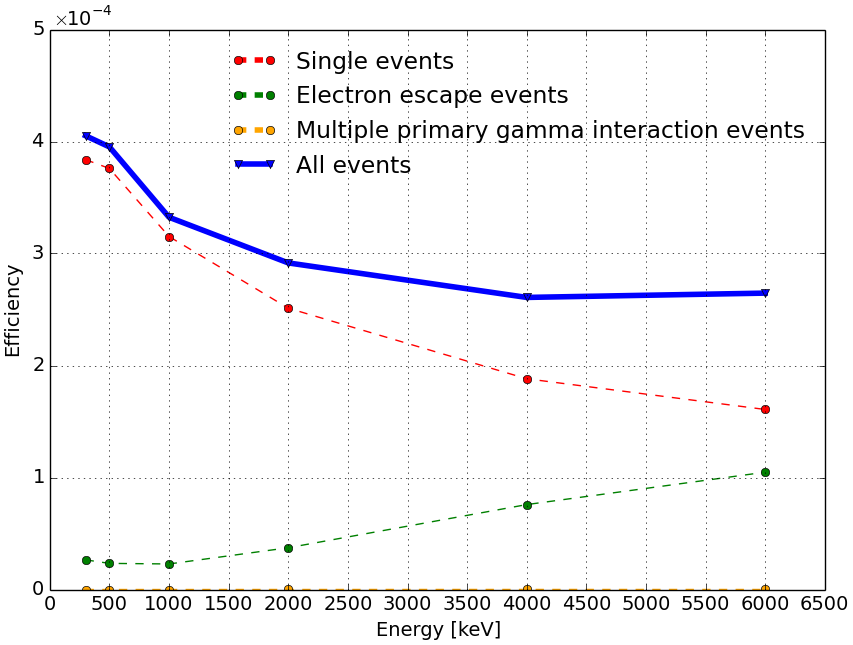
\includegraphics[width=0.7\textwidth]{./Figure/new/effVSenergy_trigger.png}
\caption{Compton camera efficiency as a function of the gamma energy for the different kind of possible events (see section~\ref{MatMeth::events}).}
\label{fig::eff_evKind}
\end{figure}

Figure~\ref{fig::efficiency_study} shows the absolute gamma detection efficiency as a function of the gamma source position with respect to the center of the camera in the transverse plane. On the left side, we show the results achieved with an ideal detector (i.e. without energy detection threshold). On the right side realistic energy thresholds are applied on each detector section.

\begin{figure} [!hbtp]	
\centering
%\subfloat[]{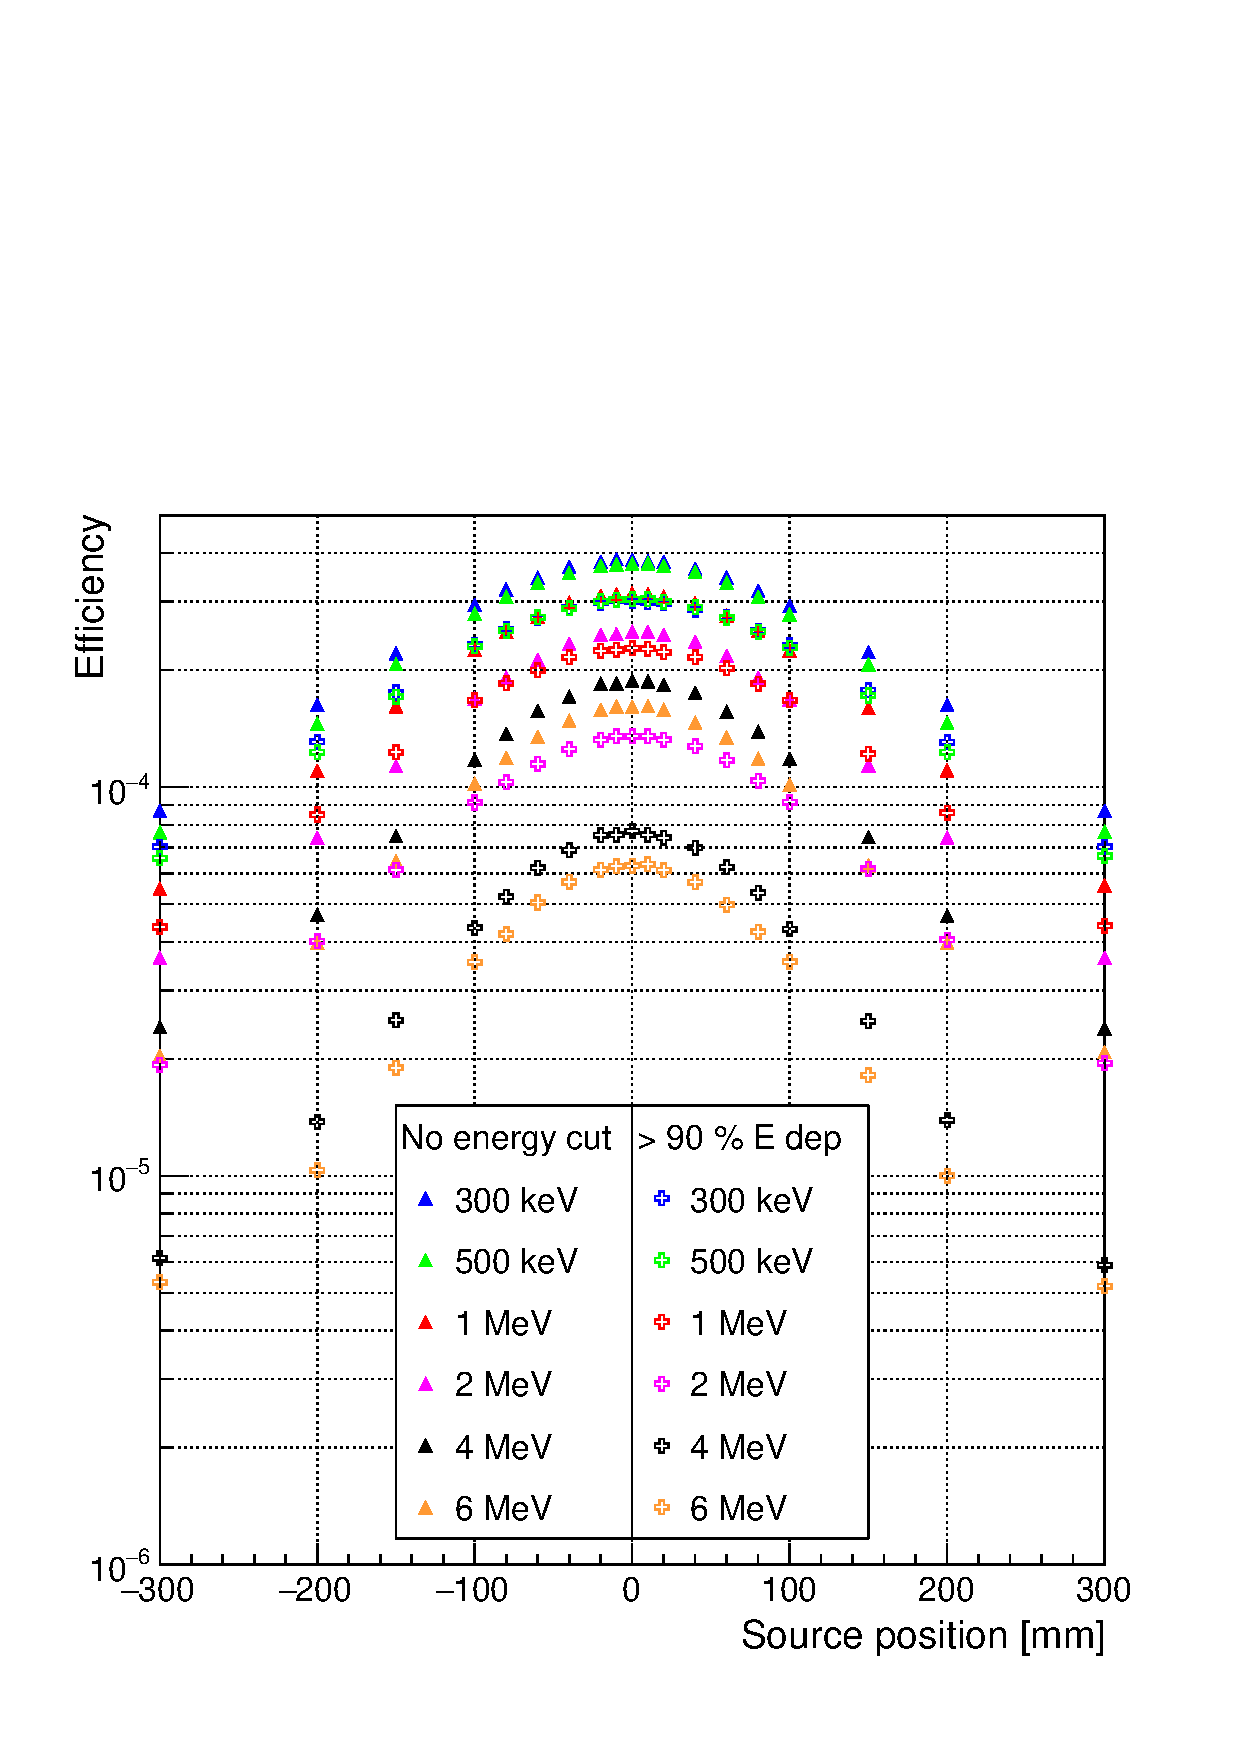
\includegraphics[width=0.5\textwidth]{./Figure/new/EffVSpos_withSumCut.pdf}}
\subfloat[]{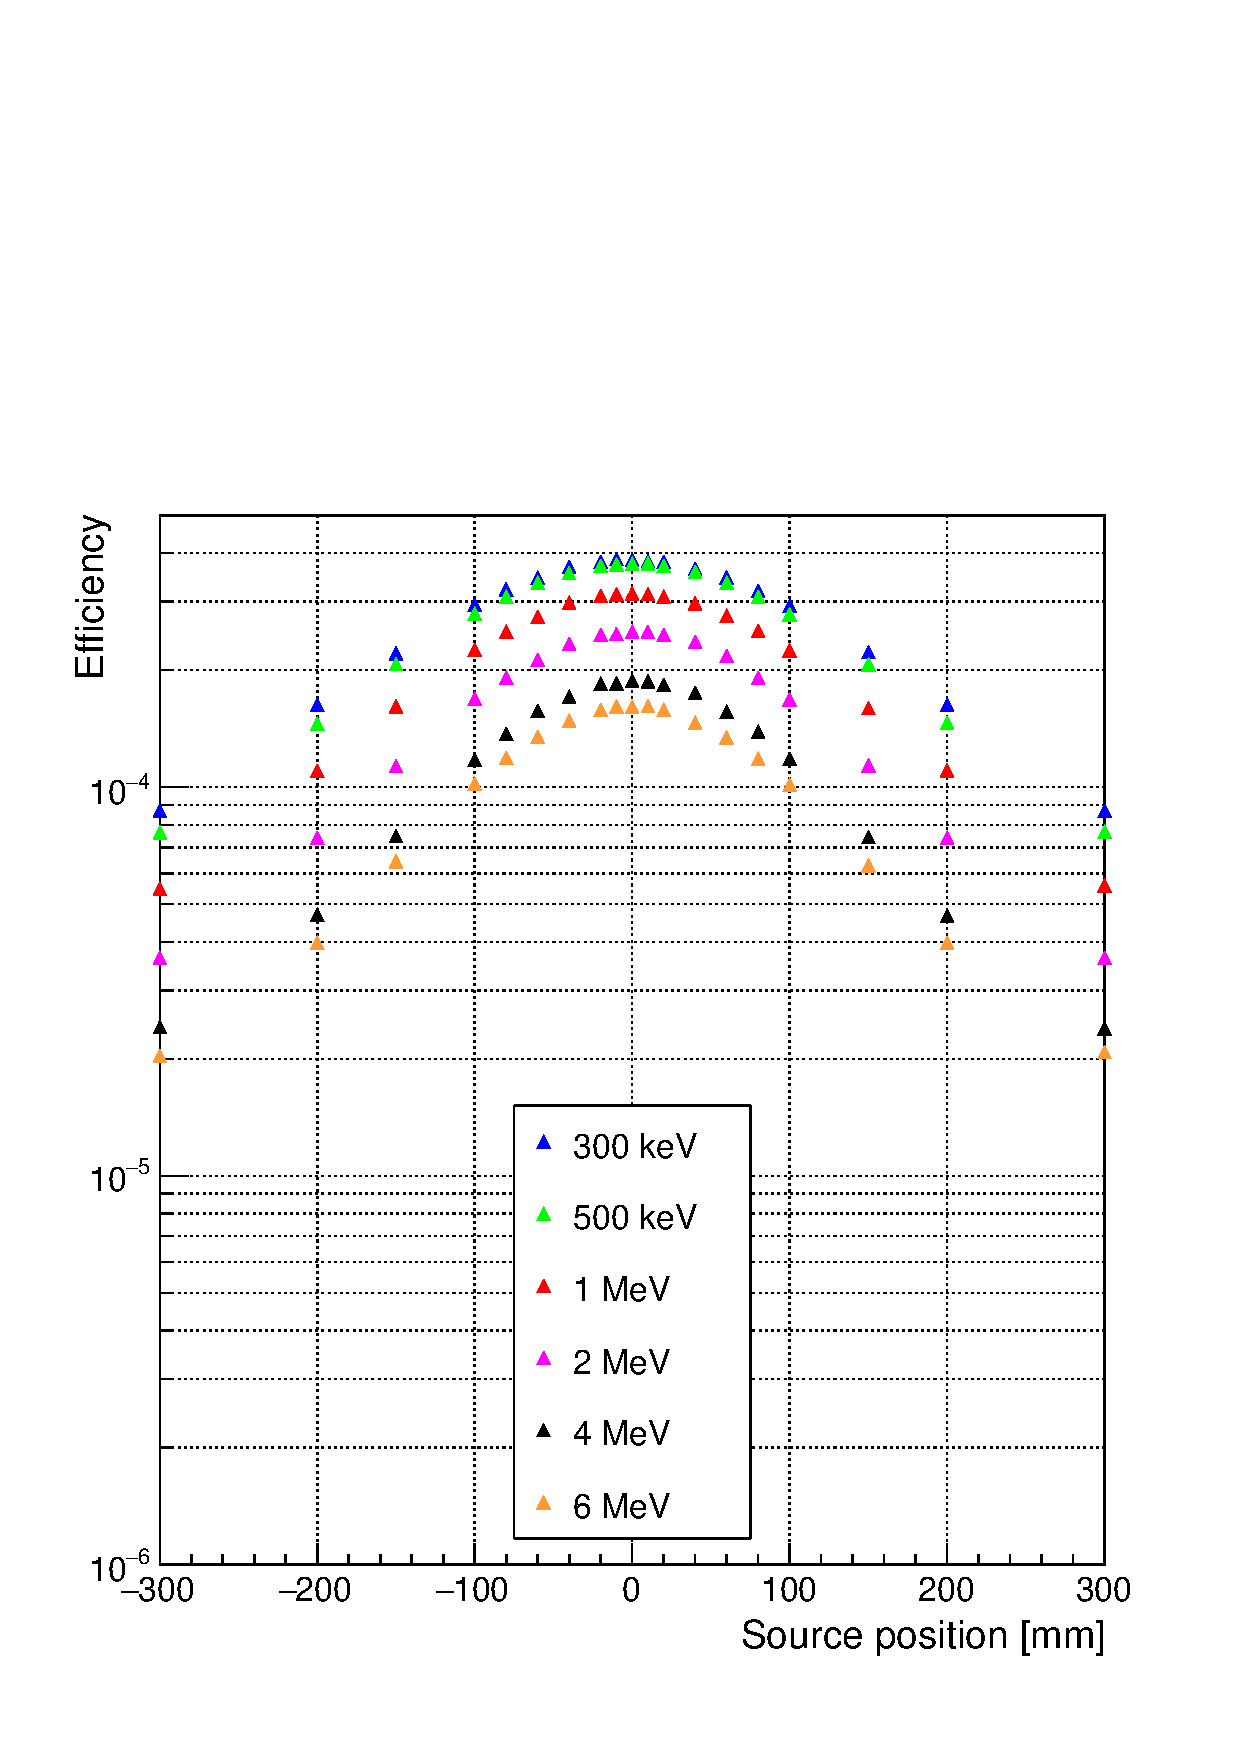
\includegraphics[width=0.5\textwidth]{./Figure/new/EffVSpos_noCut_simple.pdf}}
%\subfloat[]{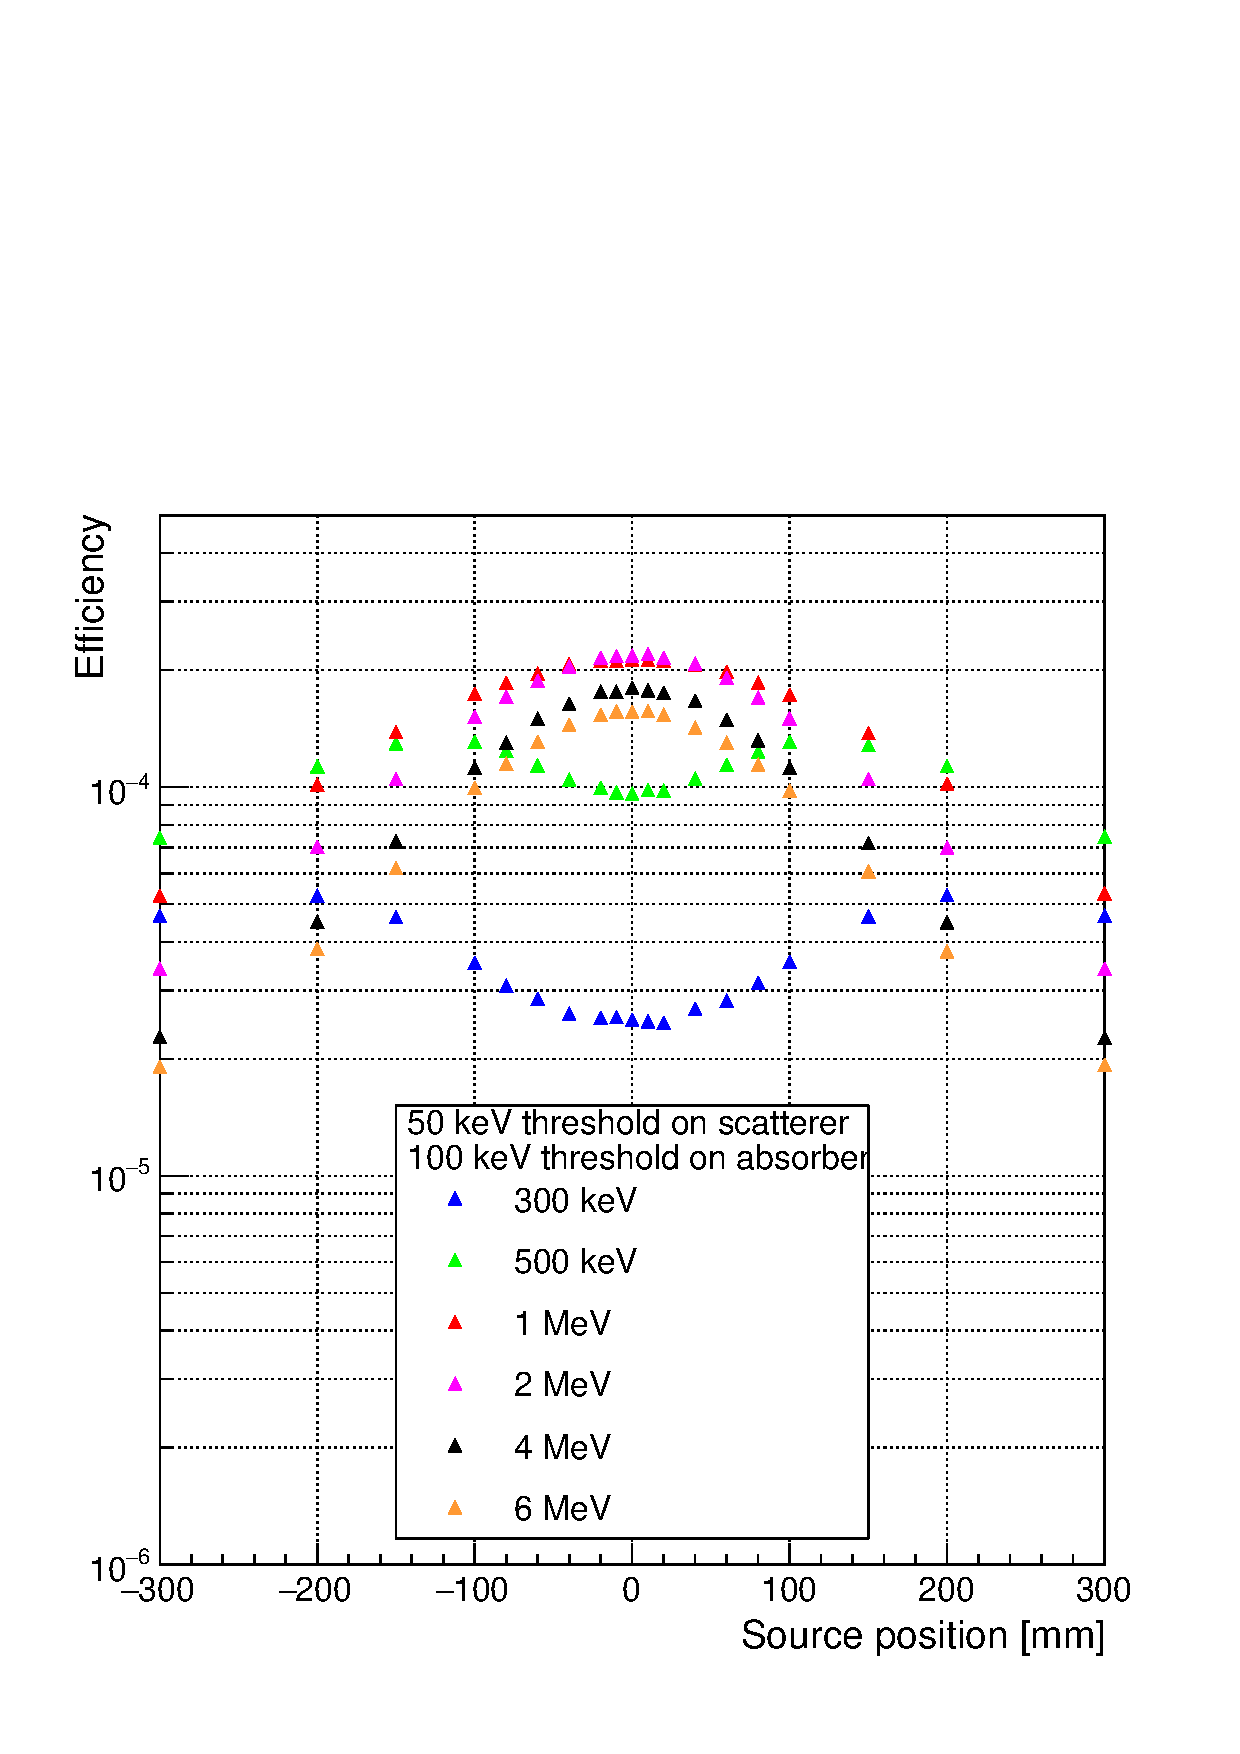
\includegraphics[width=0.5\textwidth]{./Figure/new/EffVSpos_withSingleCut.pdf}}
\subfloat[]{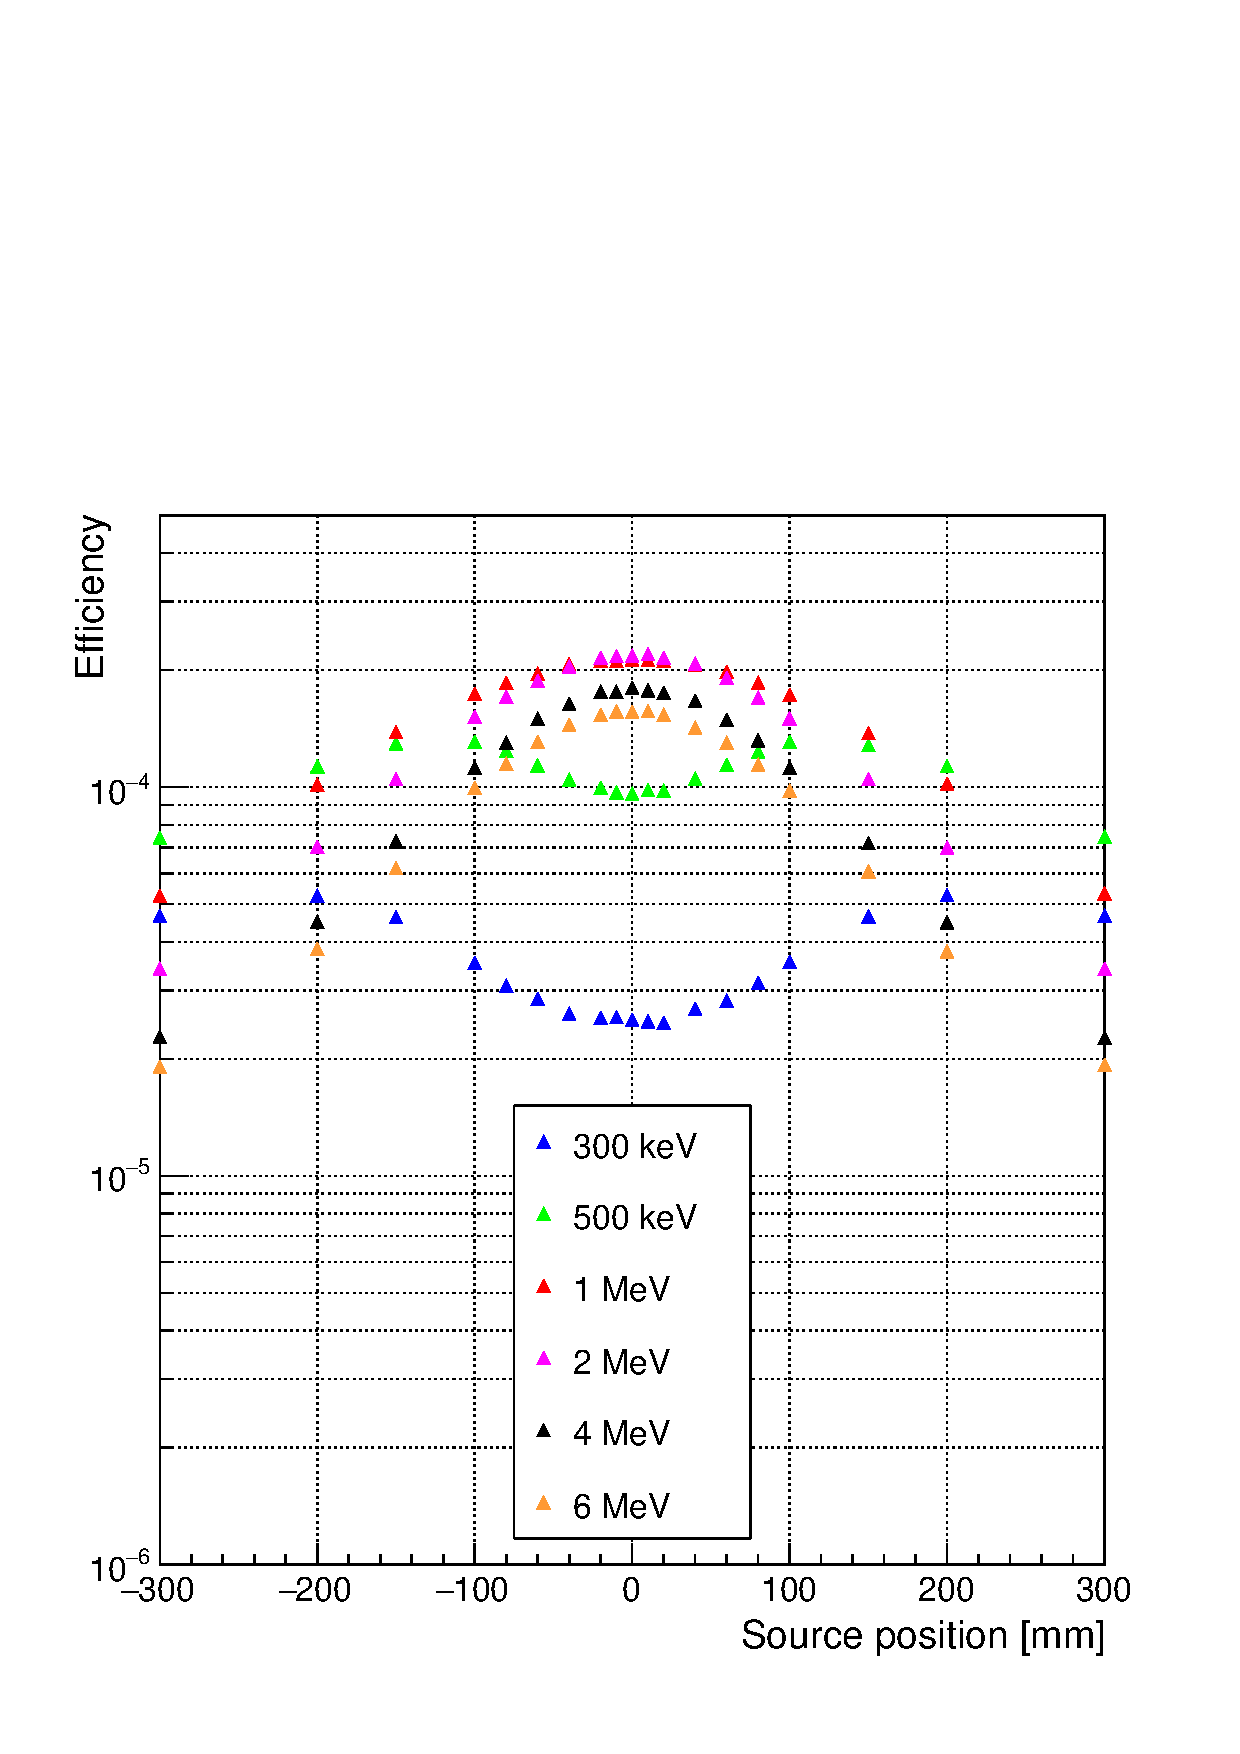
\includegraphics[width=0.5\textwidth]{./Figure/new/EffVSpos_CutSingle_simple.pdf}}
\caption{Absolute Compton camera efficiency as a function of the gamma source position for different gamma energies, in the range between 300~keV to 6~MeV. The left side shows the camera efficiency with no detection energy threshold. In the right side, detection energy thresholds are applied to reproduce a realistic scenario (lower limit of 50~keV for the scatterer, 100~keV for the absorber). These values can change for the final configuration, according to the detector energy resolutions achieved.}
\label{fig::efficiency_study}
\end{figure}

As expected according to the interaction probability energy dependency, the efficiency is higher for low gamma energies, and it lies in the range $4\times10^{-4}$ at 300~keV and $1.5\times10^{-4}$ at 6~MeV at the center of the camera. Moreover, it can be noticed how the efficiency slightly drops as the point source is shifted away from the camera center: efficiency reductions at 500~keV and 4~MeV are respectively of 25\% and 35\% with the source at 300~mm distance from the camera center, with respect to the value detected in central position. This effect is more important for high energies, for which the incident gamma is less deflected in the scatterer for the same energy deposited compared to a low energy gamma (see equation~\ref{Compton_equation}).\\  
Figure~\ref{fig::efficiency_study}(b) shows the effect of realistic camera detection thresholds as opposed to ideal detection. The gamma detection efficiency drops of a factor ranging from about 1.25 to more than an order of magnitude for the central detection area for energies in the range 300~keV to 2~MeV respectively. The effect is reduced by the distance of the source from the center of the camera. Negligible effects are detected for positions with a distance greater than 200~mm from the center of the camera, and for any distance at energies above 2~MeV, while the efficiency is reduced in the central area of the camera for energies below 4~MeV.\\

\begin{figure} [!hbtp]	
\centering
%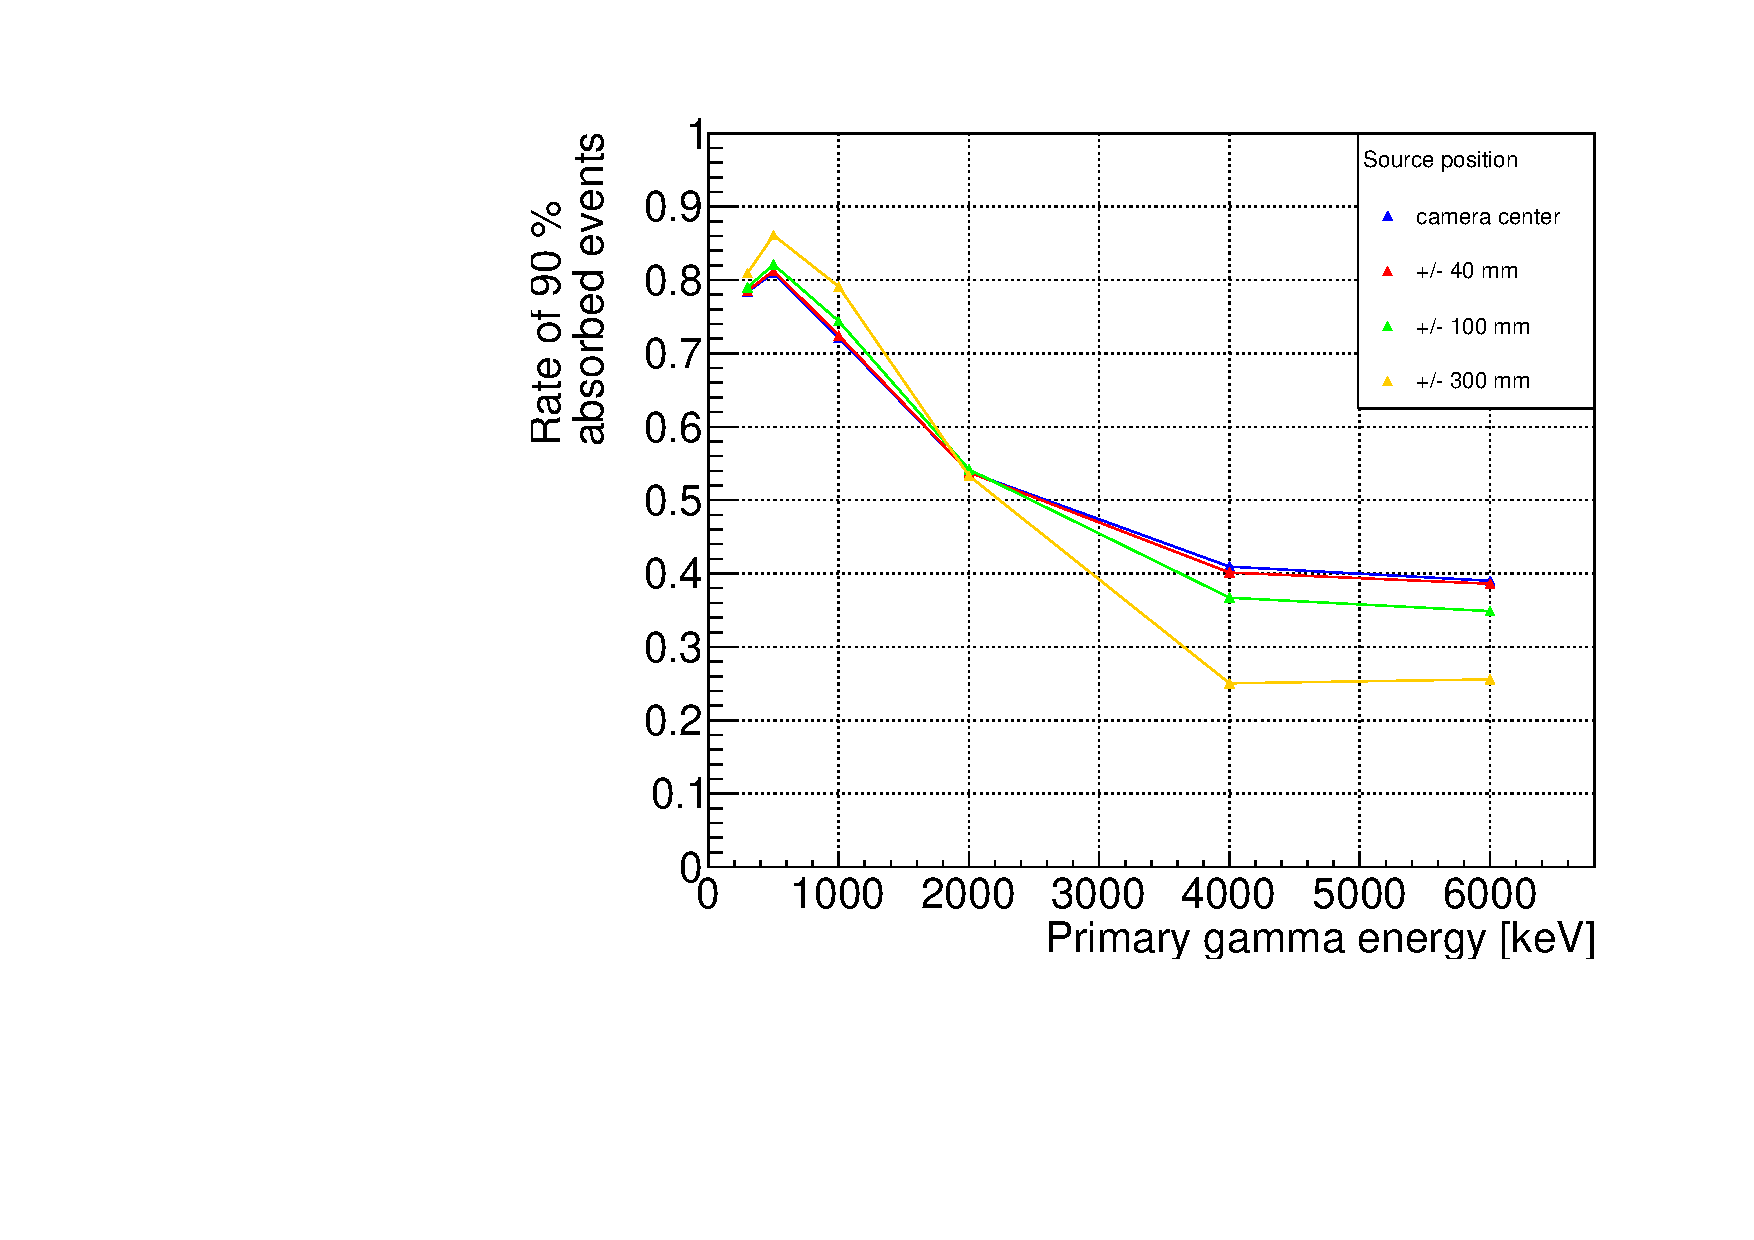
\includegraphics[width=0.7\textwidth]{./Figure/new/rate_90percent_energy_4distances.pdf}
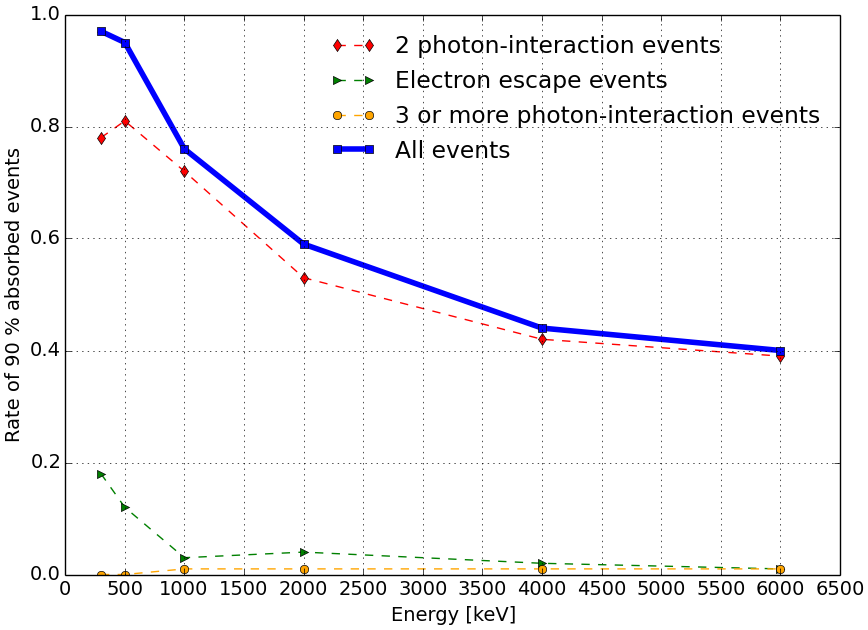
\includegraphics[width=0.7\textwidth]{./Figure/new/90absFracVSenergy_hadronth.png}
\caption{Ratio between coincidence events with more than 90\% of the primary photon energy absorbed in the detector layer and all detected coincidences for 4 source positions: center of the camera, 40, 100, 300~mm from the center.}
\label{fig::rate_full_abs}
\end{figure}

Figure~\ref{fig::rate_full_abs} shows the rate of events with more than 90\% of the primary gamma energy deposited in the detector layers; the source is placed in the center of the camera transverse surface, and no selection are applied on a single detector layer basis. The rate of 90\% absorbed events is reported for the different kinds of detected events. As expected, the rate of almost fully absorbed events decreases as the energy increases, in a range between more than 80\% and 40\% for 300~keV and 6~MeV primary photon energy, respectively. The most of the 90\% absorbed events single events, with the electron escape and multiple ones negligible for primary gamma energies above 1~MeV. At lower energy, the Compton recoil electron is often able to exit the scatterer layer were the Compton interaction takes place, but can be lost without further interactions, so that this kind of events is considered as single with an energy absorption below 90\%. This can explain the decrease of single almost full absorption at 300~keV. If the electron interacts with a scatterer layer, is more likely to be absorbed at low energy, explaining the increasing electron escape absorbed events below 1~MeV.  
 
\subsection{Rate of random coincidences}
\label{Results::beamInt}
 
In figure~\ref{fig:coincidences}, the different components of the signal resulting from the PMMA exposure to proton and carbon ion beams are shown as a function of the beam intensity. The true coincidences represent scatterer-absorber time coincidences generated by the same gamma ray (only single events). All the other coincidence types compose the background. The collected data sets are reported with and without the applied time-of-flight discrimination, mainly employed for neutron rejection, as mentioned in section~\ref{MatMeth::TOF_Ecut}.


\begin{figure} [!h]
  %\subfloat[]{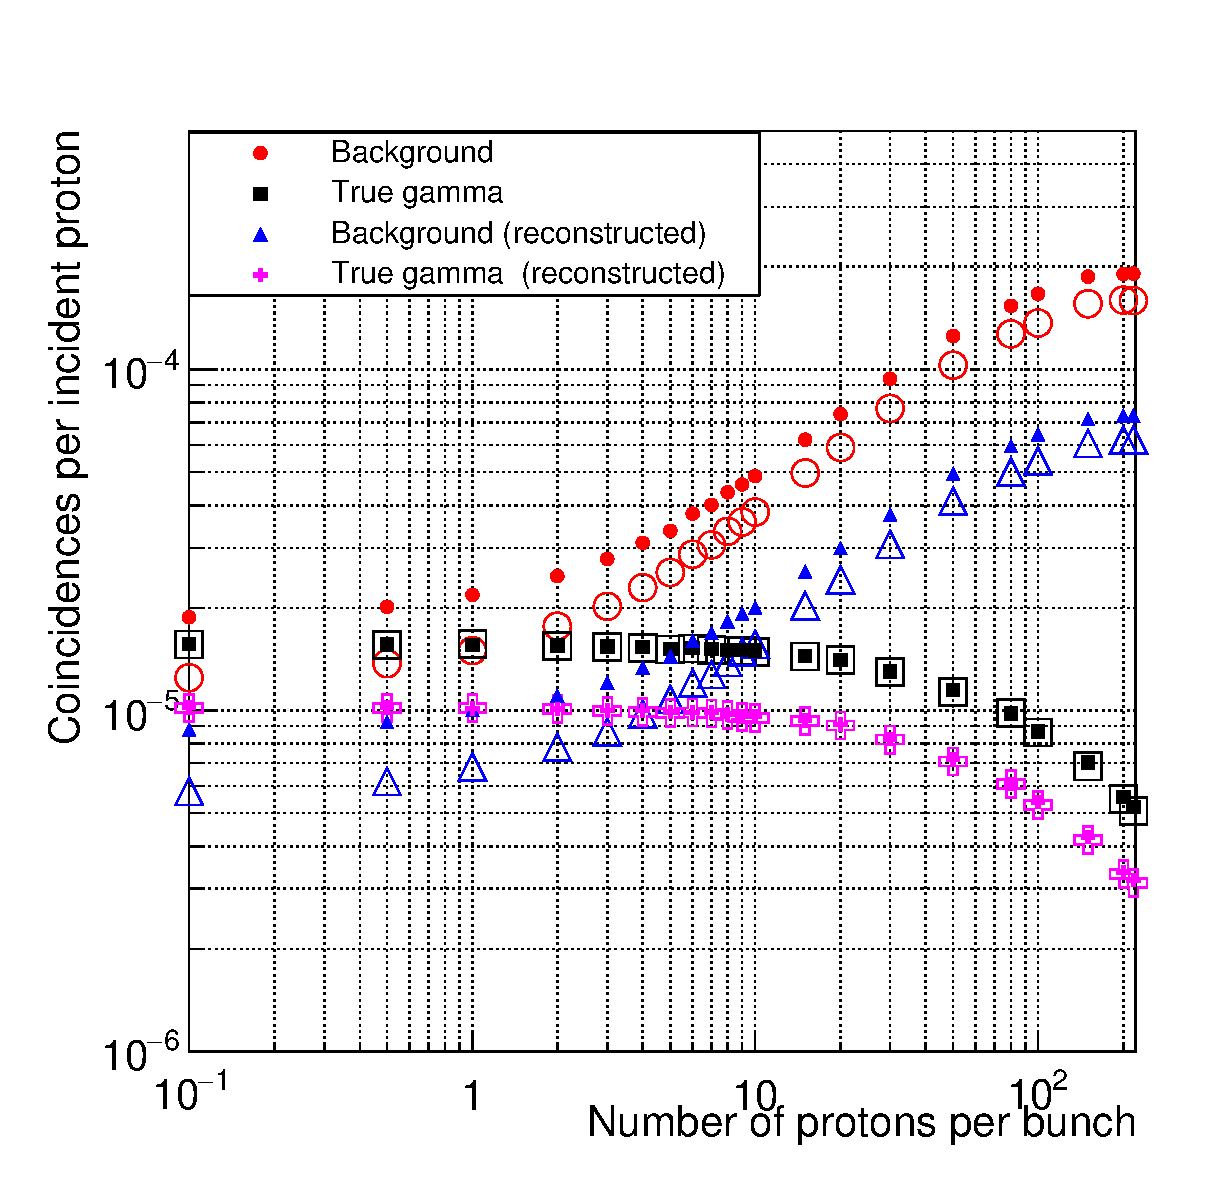
\includegraphics[width=0.5\textwidth]{./Figure/2017_06_28_Taux_coincidences_variation_protons_New_design_4EntreesLegend_LogXLogY.eps}}
  \subfloat[]{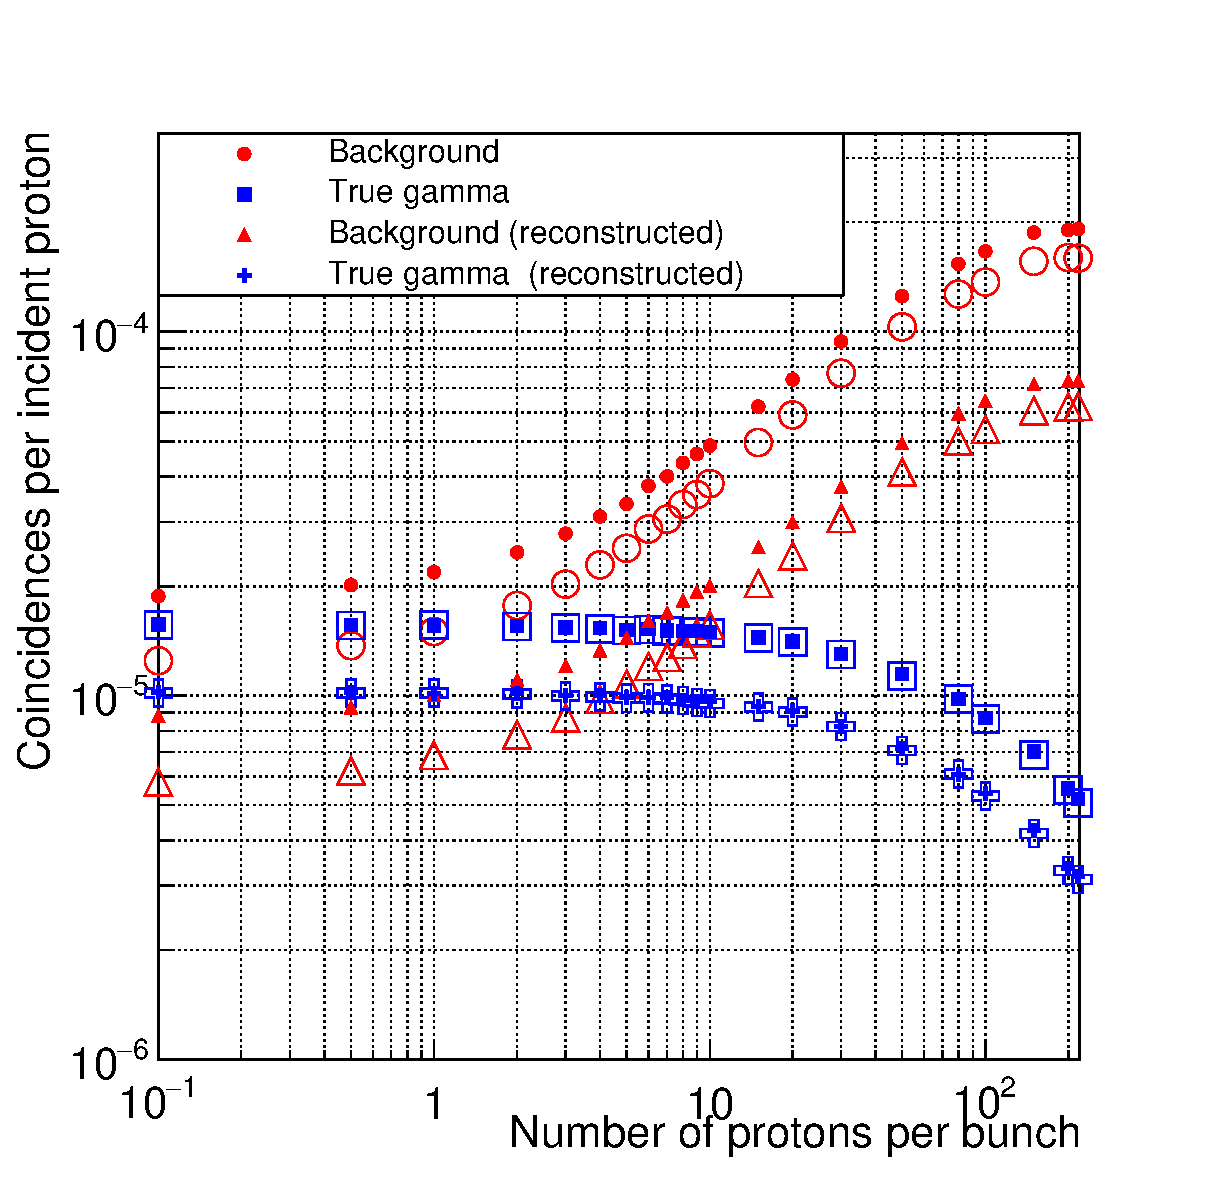
\includegraphics[width=0.5\textwidth]{./Figure/new/coincYields_protons.eps}}
  %\subfloat[]{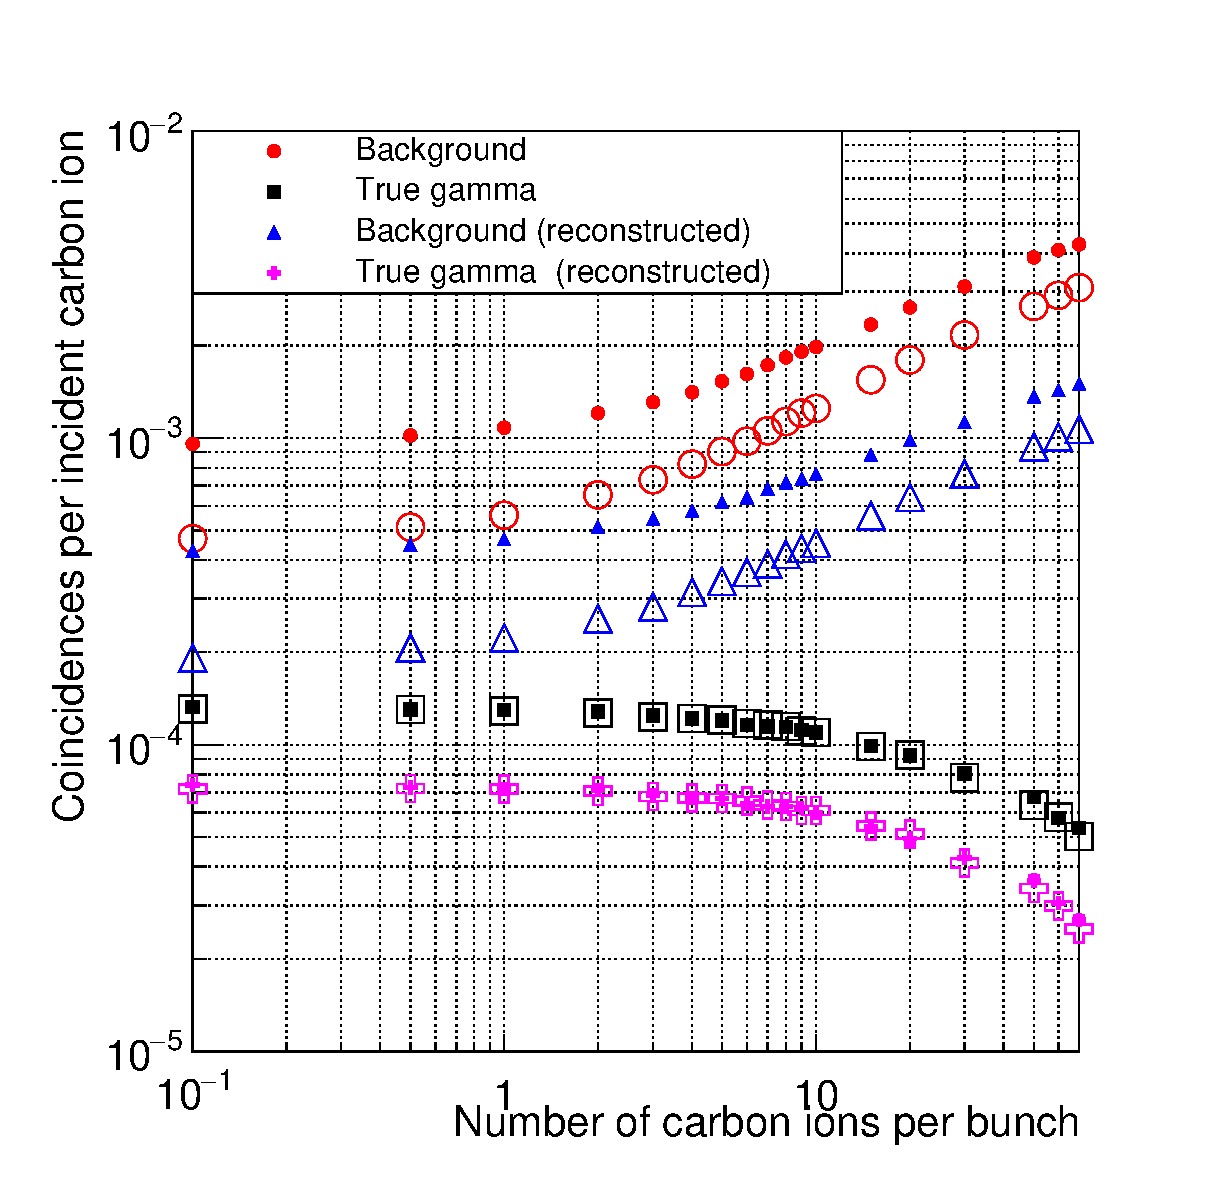
\includegraphics[width=0.5\textwidth]{./Figure/2017_06_28_Taux_coincidences_variation_carbonIons_New_design_4EntreesLegend_LogXLogY.eps}}
  \subfloat[]{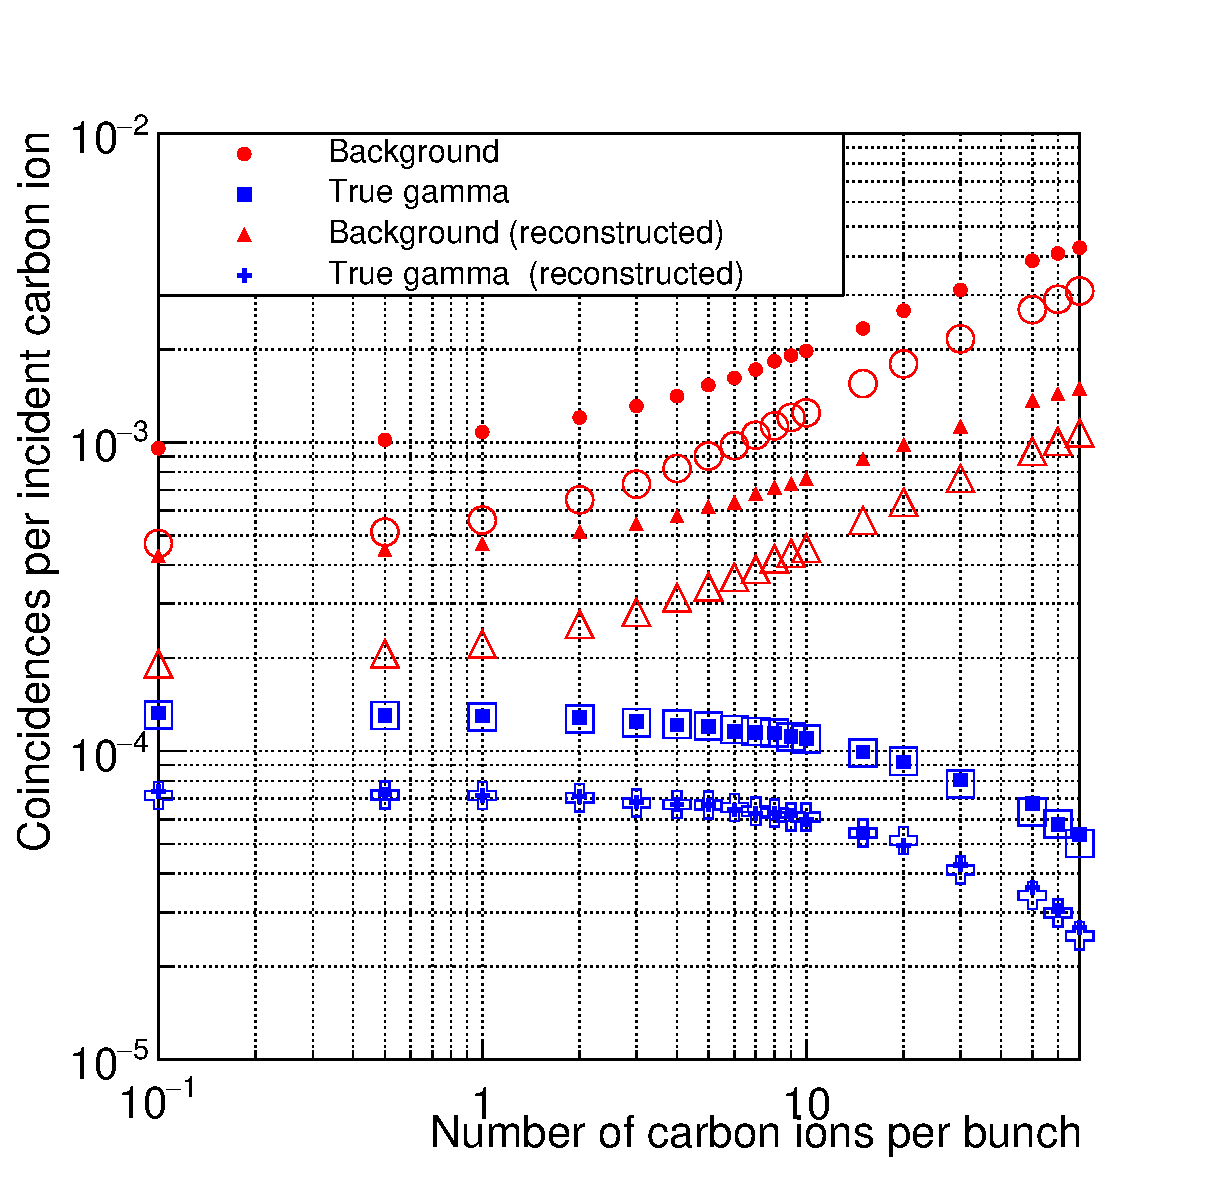
\includegraphics[width=0.5\textwidth]{./Figure/new/coincYields_Cions.eps}}
  \caption{Coincidences yield for protons (left) and carbon ions (right) as a function of the beam intensity. The intensity is reported as number of incident particles per bunch. The filled markers correspond to the collected data without time-of-flight discrimination, while this cut is applied to the data reported with empty markers. Moreover, the yields are given before and after the profile reconstruction with the line-cone algorithm.}
  \label{fig:coincidences}
\end{figure}

In figure~\ref{fig:coincidences}(a) and (b) the amount of true gamma coincidences and background events are reported before and after reconstruction via line-cone algorithm as a function of the beam intensity for proton (a) and carbon ion (b) beams. In addition to this, for each curve realized with the complete collected data set, the related one realized after time-of-flight selection of events is sketched (empty symbols). All the curves have been normalized to the number of incident ions.

The amount of background events (mainly random coincidences) increases with the increasing beam intensity: a factor of about 30 with respect to true gamma events is obtained for proton beams at  the intensity of 200 protons per bunch with no event selection, while a factor more than two times higher is reported for carbon ions in the same conditions. The time-of-flight selection can slightly improve the signal -over-noise ratio by reducing the amount of background events. The amount of true gamma events and background events becomes similar at the intensity of about 1 proton per bunch.


\subsection{Camera precision}
\label{Results::precision_reconstruction}
Given the results presented in the previous section, the camera precision in the fall-off identification is investigated with proton beams at reduced intensities.
%The simulation setup shown in figure~\ref{fig:fig_setup_CC_simulation_Hadronth} has been implemented to test the line-cone analytic reconstruction method and compare it to the iterative LM-MLEM algorithm~\cite{maxim_filtered_2014,hilaire_compton_2014}. 
A single data set has been collected, corresponding to the irradiation of the PMMA phantom with a monoenergetic 160~MeV  proton beam, with a reduced intensity of 1 proton per bunch in average. A total of $10^{10}$ protons has been simulated to define the reference PG profile, and then different low statistics profiles have been produced for the precision estimate as explained in section~\ref{MatMeth:precision}. 

The high statistics profile reconstructed via line-cone algorithm is shown in figure~\ref{fig:fig_Results_Estimation_Camera_Profil_highStat_CC_simulation_Hadronth_LineCone} and via the LM-MLEM reconstruction method in figure~\ref{fig:fig_Results_Estimation_Camera_Profil_highStat_CC_simulation_Hadronth_MLEM}. A NURBS fit of a low statistics sample ($10^8$ incident protons) is shown in figures~\ref{fig:fig_Estimation_Camera_CC_NURBS_Poisson_LC} for the line cone and~\ref{fig:fig_Estimation_Camera_CC_NURBS_Poisson_MLEM} for the MLEM.
%Figures~\ref{fig:fig_Results_Chi2_Distribution_Variation_CC_simulation_Hadronth_LC} and~\ref{fig:fig_Results_Chi2_Distribution_Variation_CC_simulation_Hadronth_MLEM} show the distribution of $\chi^2$ calculated for a low statistic profile at $10^8$ incident protons. 
The retrieved optimal shift distribution is shown in figure~\ref{fig:fig_Results_Precision_Distribution_Variation_CC_simulation_Hadronth_LC} and~\ref{fig:fig_Results_Precision_Distribution_Variation_CC_simulation_Hadronth_MLEM} for the line-cone and LM-MLEM algorithm respectively, for $10^8$ incident protons as well.
Figure~\ref{fig:comparison} shows the results of the reconstruction of the profile obtained with 10$^8$ primary protons.


\begin{figure}
  \centering
  %\subfloat[\label{fig:fig_Results_Estimation_Camera_Profil_highStat_CC_simulation_Hadronth_LineCone}]{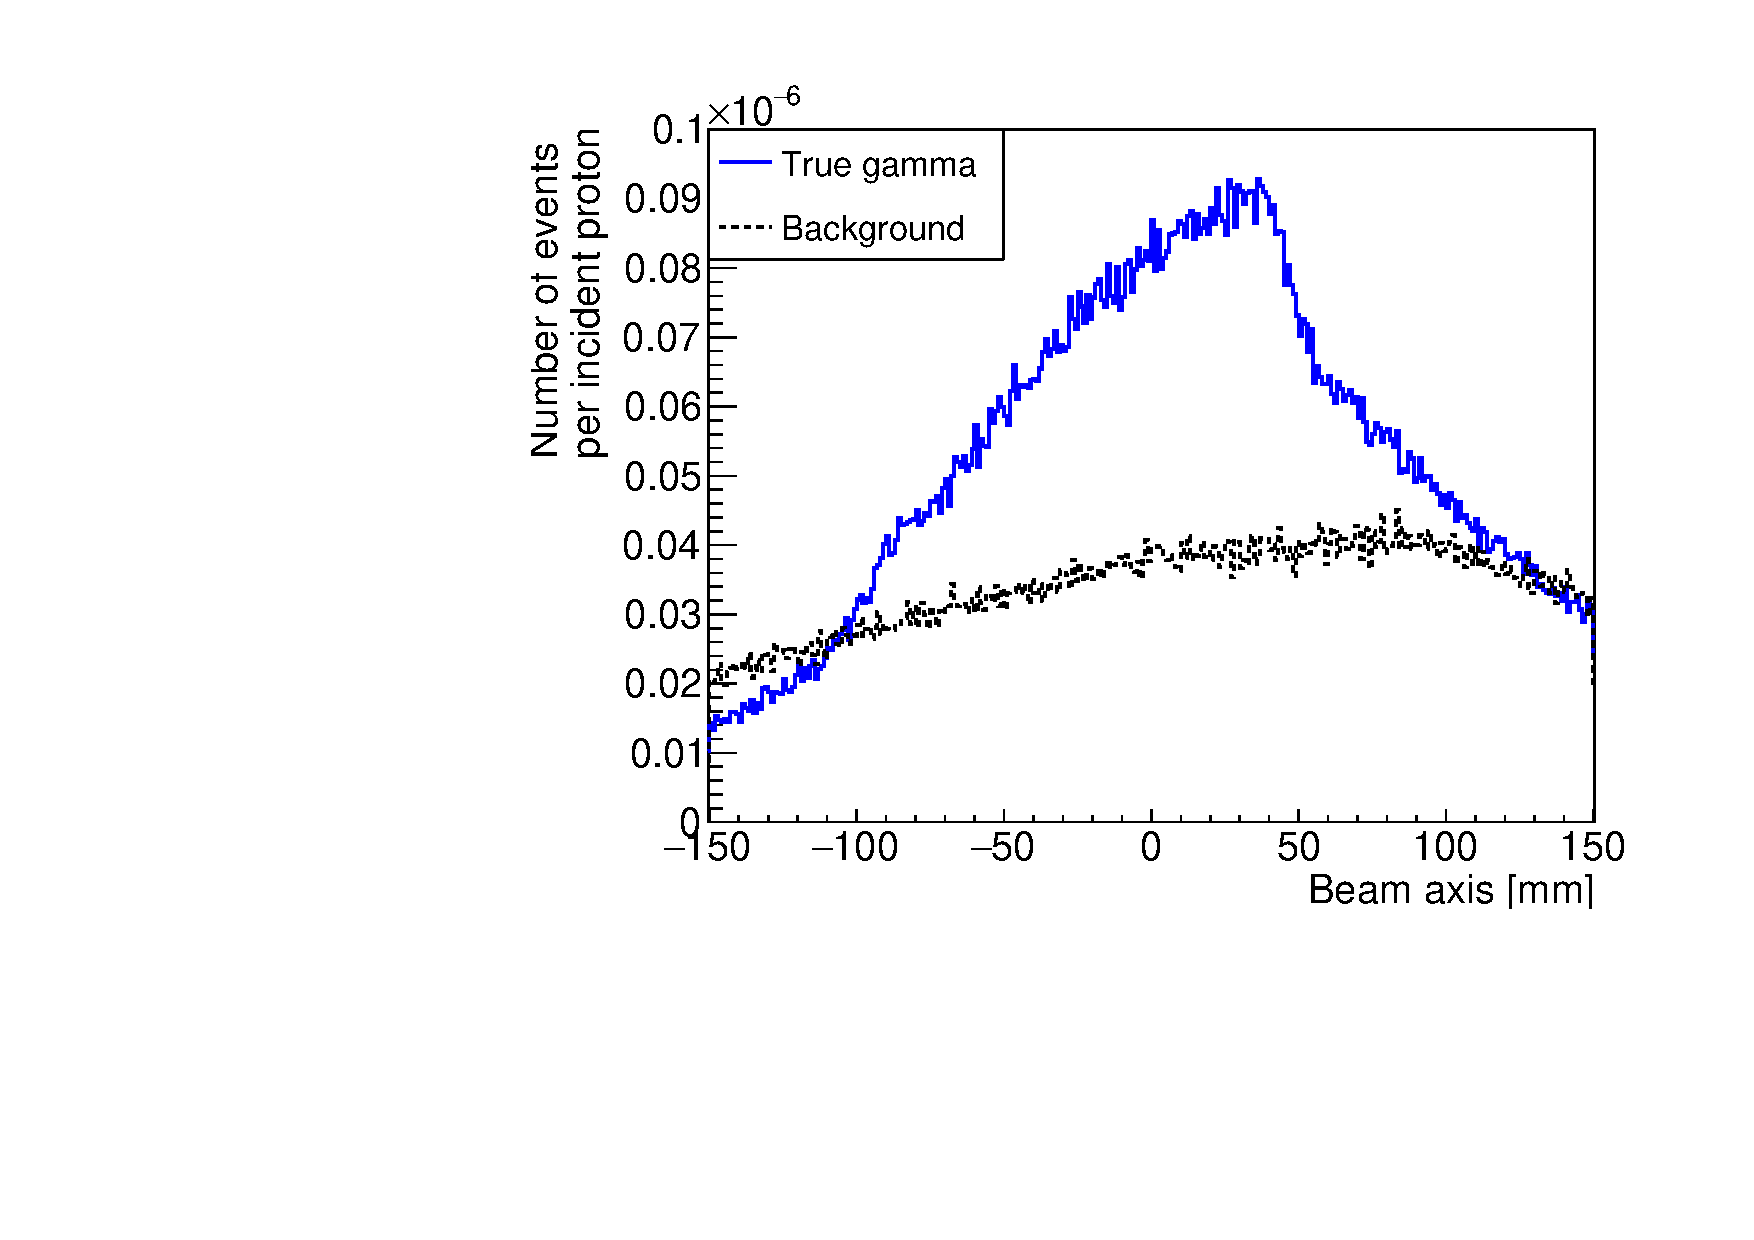
\includegraphics[width=0.48\textwidth]{./Figure/profile_high_stat_linecone_2.pdf}}
	\subfloat[\label{fig:fig_Results_Estimation_Camera_Profil_highStat_CC_simulation_Hadronth_LineCone}]{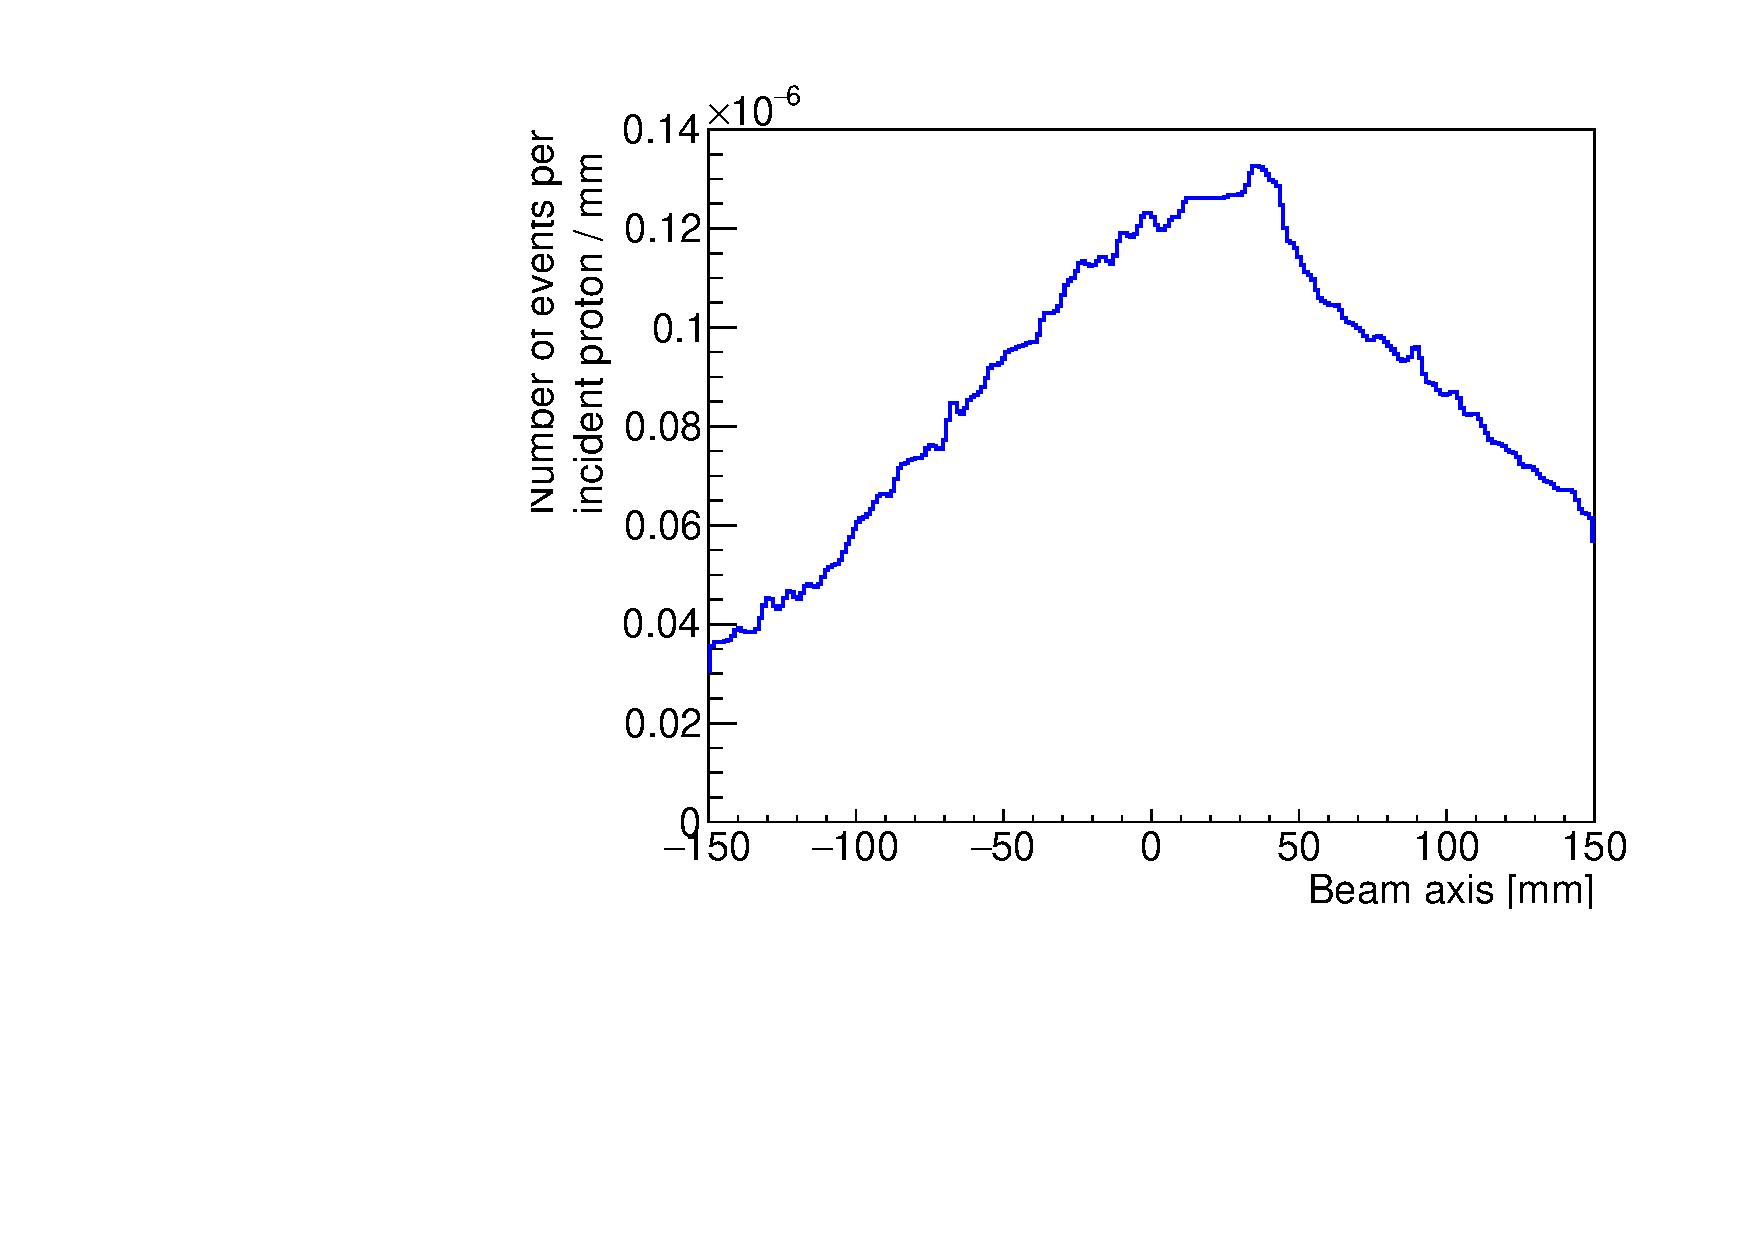
\includegraphics[width=0.48\textwidth]{./Figure/new/reconstructed_histStat_profile_lineCone_norm.pdf}}
 % \subfloat[\label{fig:fig_Results_Estimation_Camera_Profil_highStat_CC_simulation_Hadronth_MLEM}]{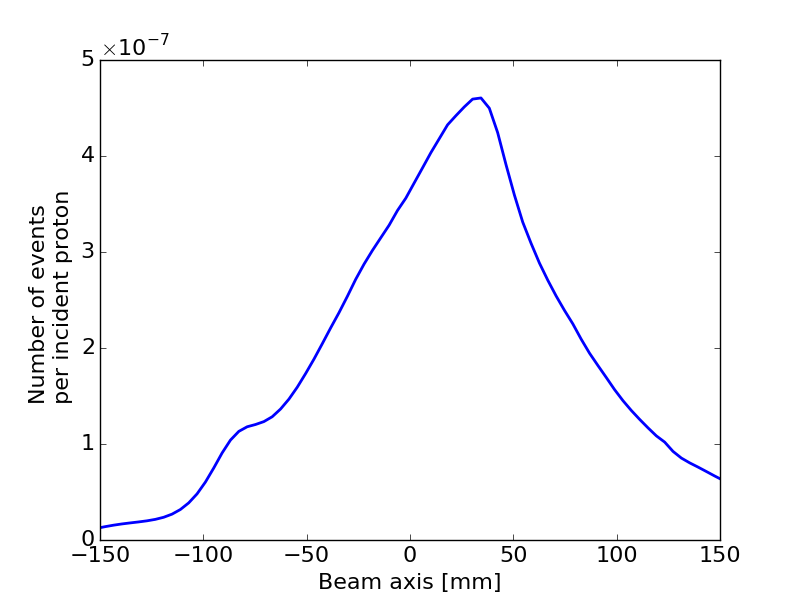
\includegraphics[width=0.48\textwidth]{./Figure/profileY_corr_r15.png}}\\
   \subfloat[\label{fig:fig_Results_Estimation_Camera_Profil_highStat_CC_simulation_Hadronth_MLEM}]{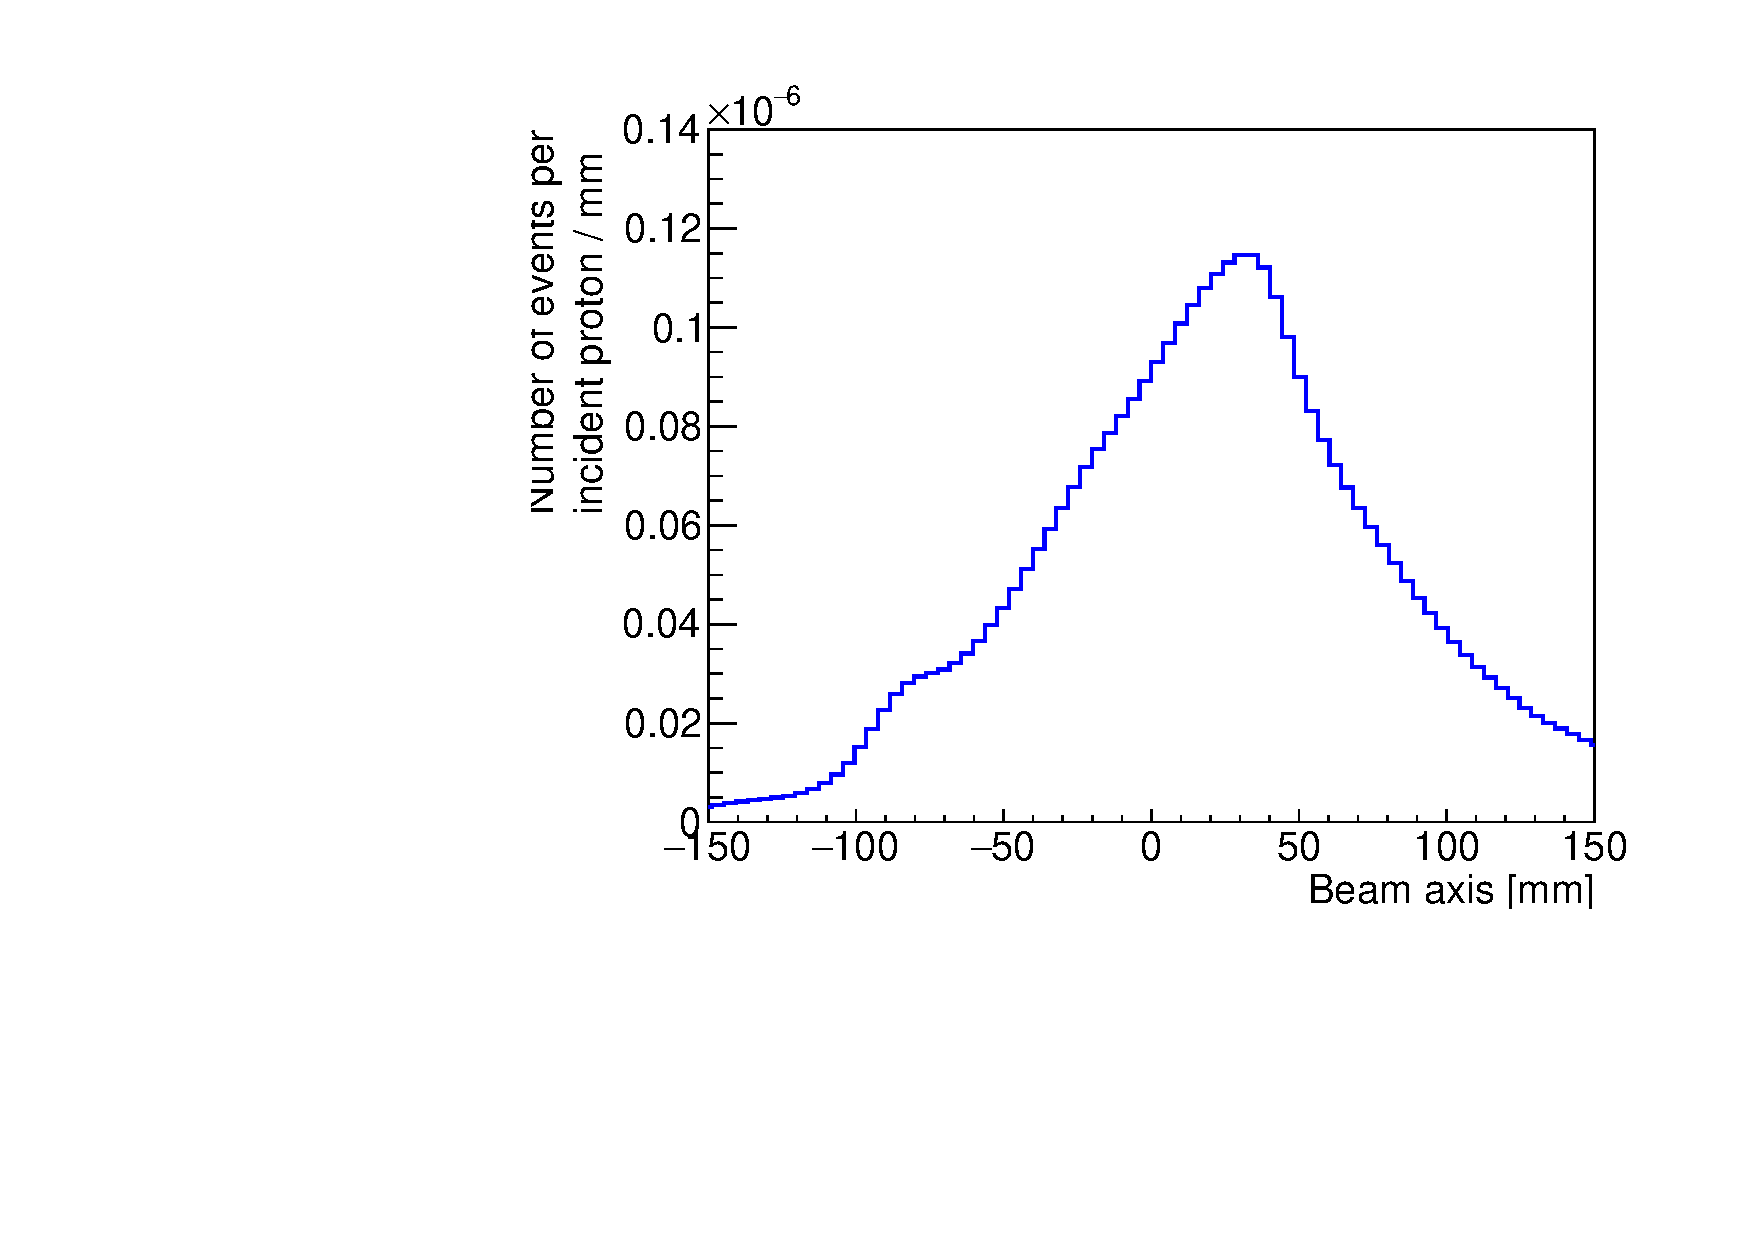
\includegraphics[width=0.48\textwidth]{./Figure/new/reconstructed_histStat_profile_norm.pdf}}\\
  % \subfloat[\label{fig:fig_Estimation_Camera_CC_NURBS_Poisson_LC}]{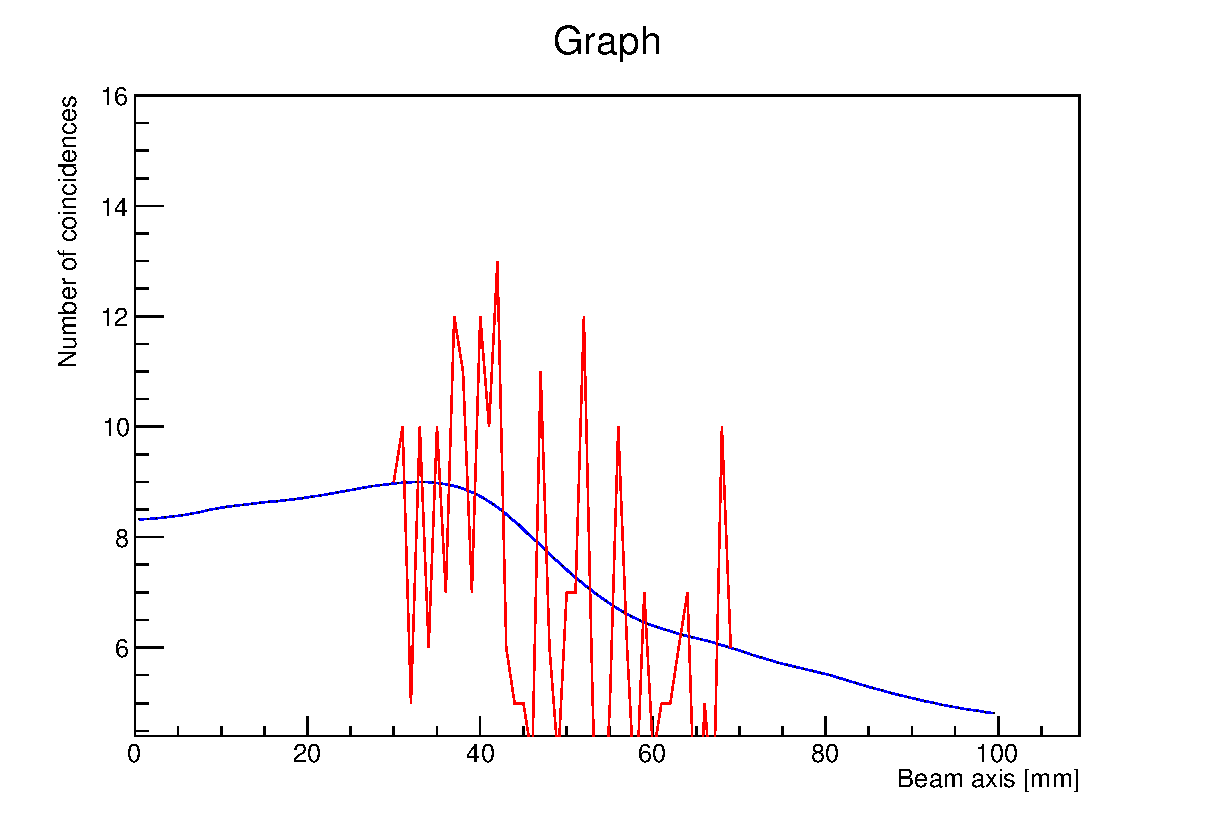
\includegraphics[width=0.33\textwidth]{./Figure/2017-08-02_Poisson_Nurbs_1e8_Article_LC.eps}}
  \subfloat[\label{fig:fig_Estimation_Camera_CC_NURBS_Poisson_LC}]{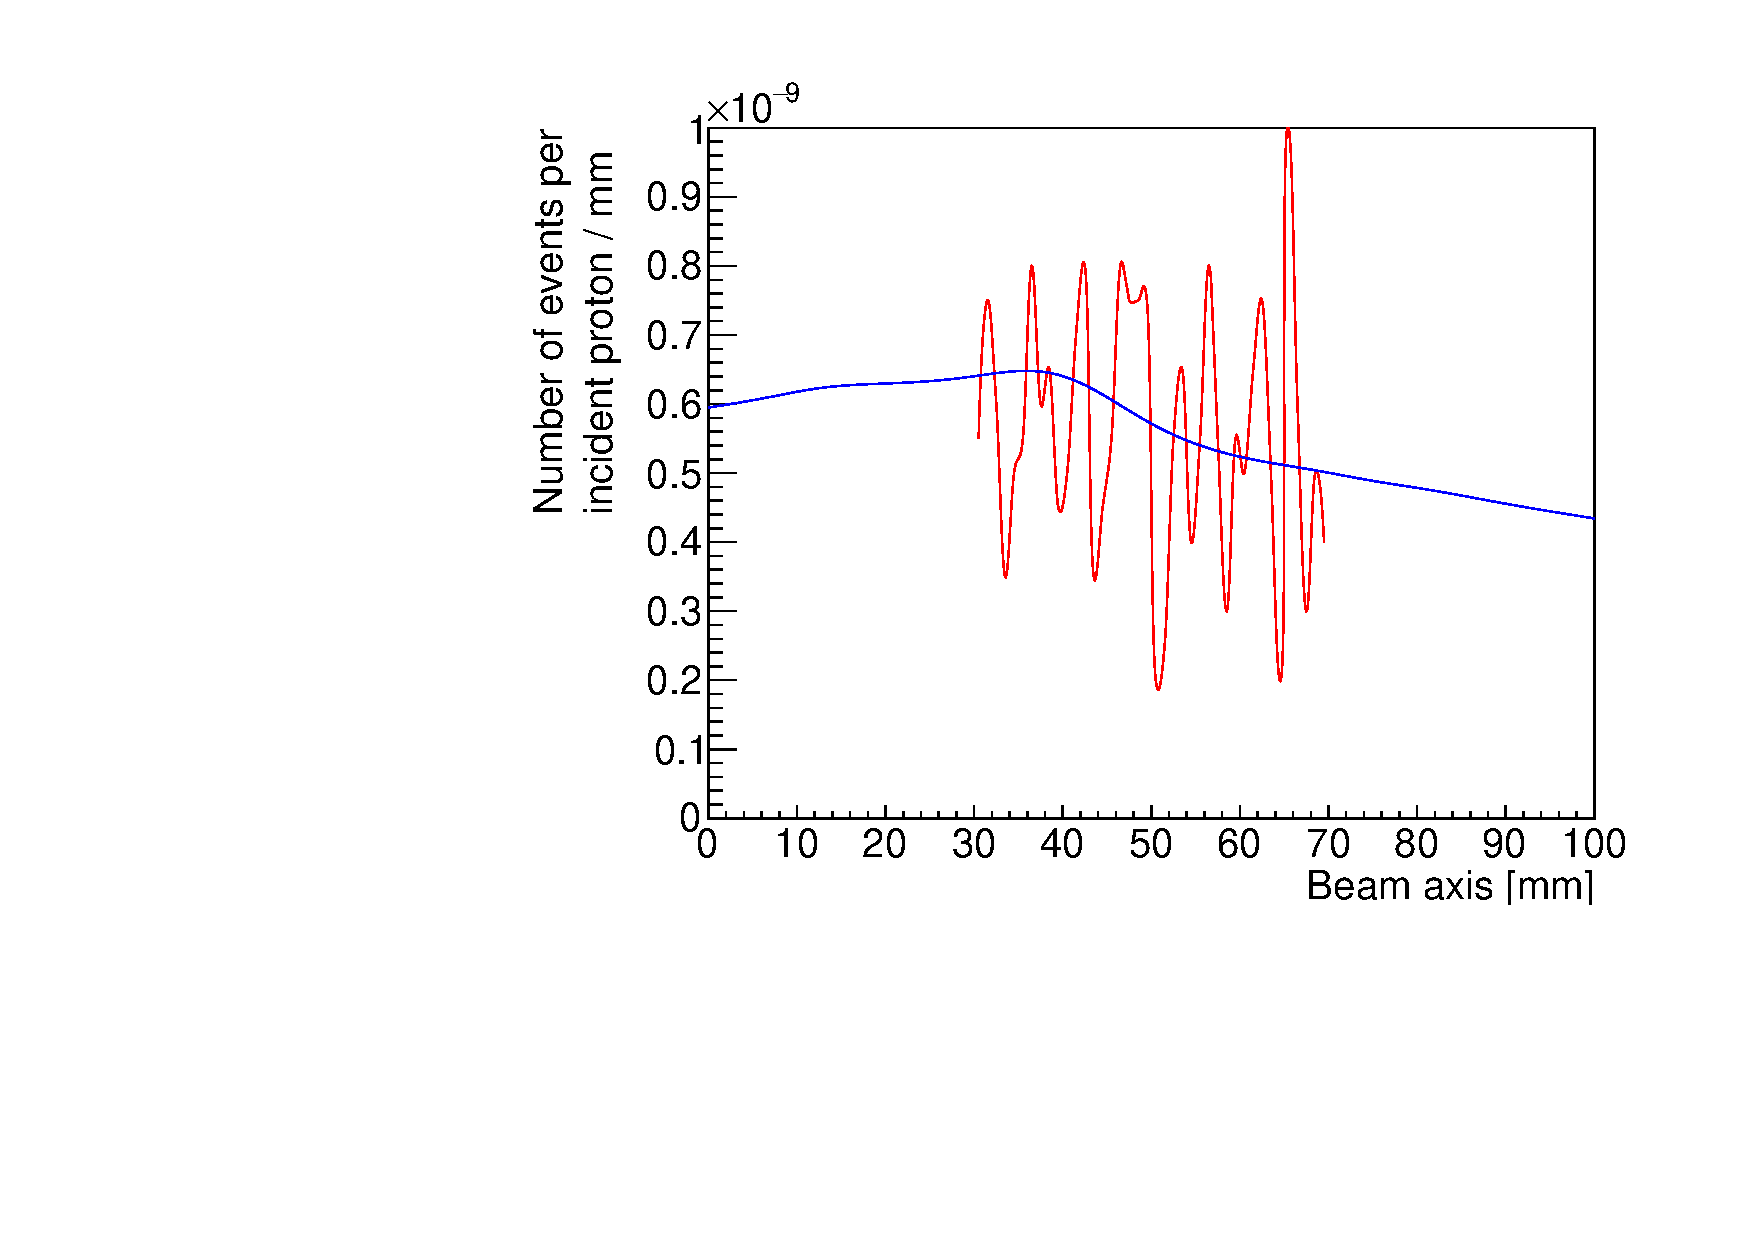
\includegraphics[width=0.48\textwidth]{./Figure/new/line_cone_refPoisson.pdf}}
  %{./Figure/line_cone_NURBS.png}}
  % \subfloat[\label{fig:fig_Estimation_Camera_CC_NURBS_Poisson_MLEM}]{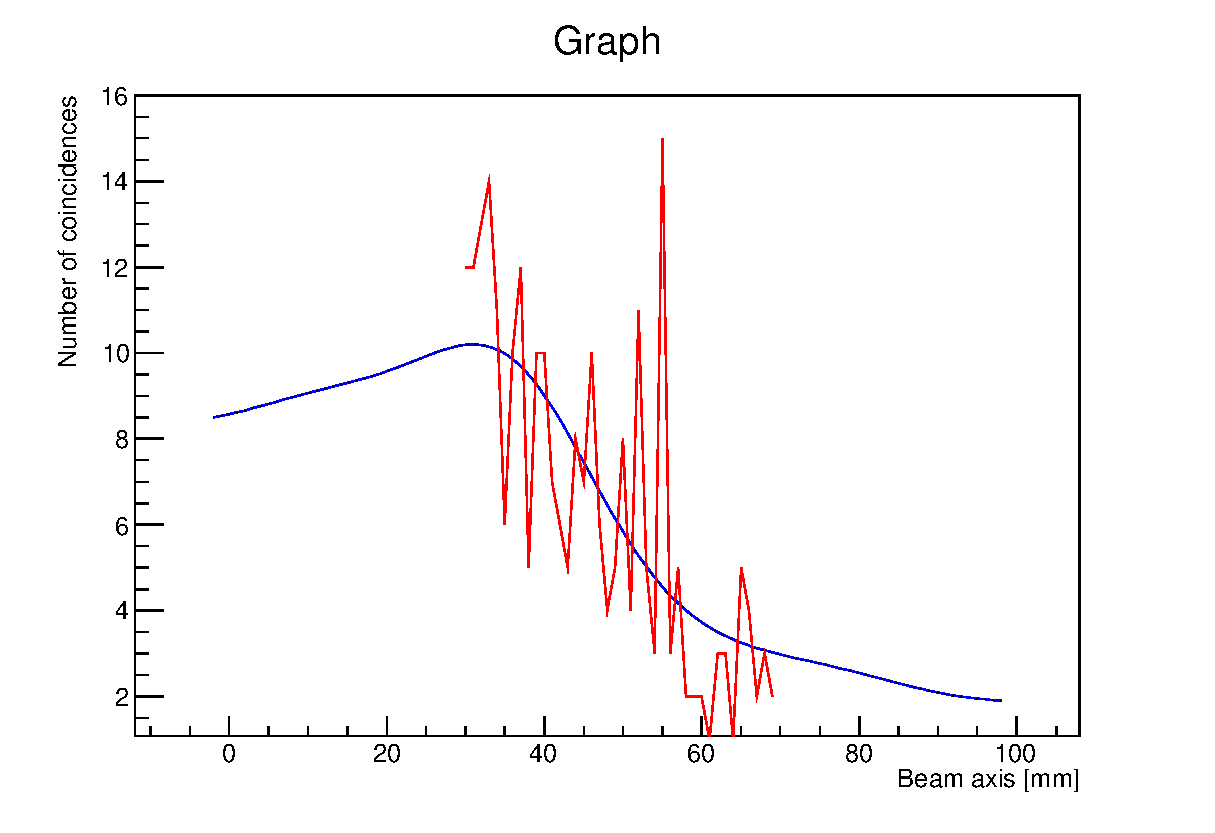
\includegraphics[width=0.33\textwidth]{./Figure/2017-08-02_Nurbs_Poisson_1e8_Article_MLEM.eps}}\\
  \subfloat[\label{fig:fig_Estimation_Camera_CC_NURBS_Poisson_MLEM}]{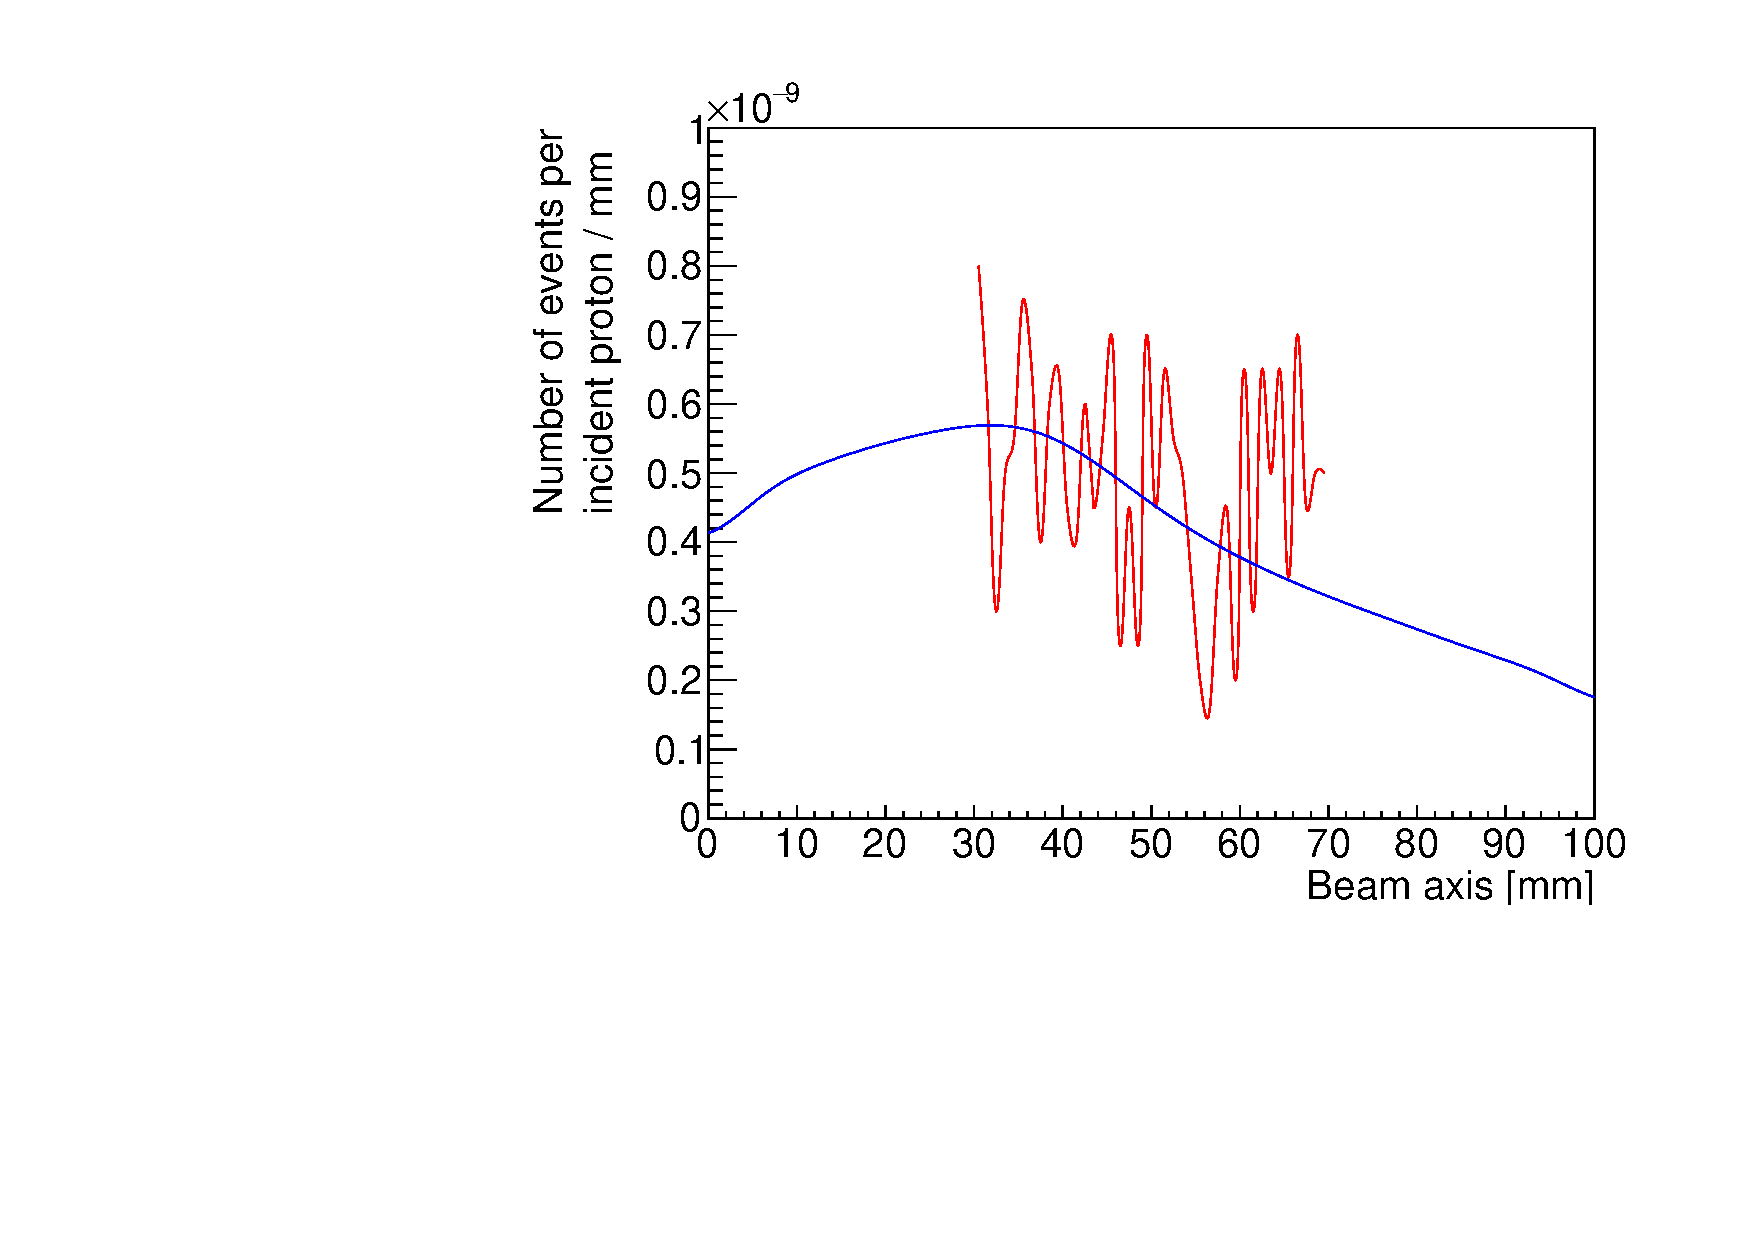
\includegraphics[width=0.48\textwidth]{./Figure/new/MLEM_refPoisson.pdf}}
  %{./Figure/MLEM_NURBS.png}}\\
  \caption{Data processing comparison for the same proton simulation with the line cone algorithm (left column) and the LM-MLEM algorithm (right column). The first row gives the reconstructed reference profile for $10^{10}$ incident protons. The second row shows the NURBS curve (blue) obtained after the normalization to a $10^8$ incident protons statistics and the profile realization with the addition of Poisson statistical fluctuations (red).}% at the same statistics of $10^8$ incident protons.}
\end{figure}

\begin{figure}
  \centering
  % \subfloat[\label{fig:fig_Results_Chi2_Distribution_Variation_CC_simulation_Hadronth_LC}]{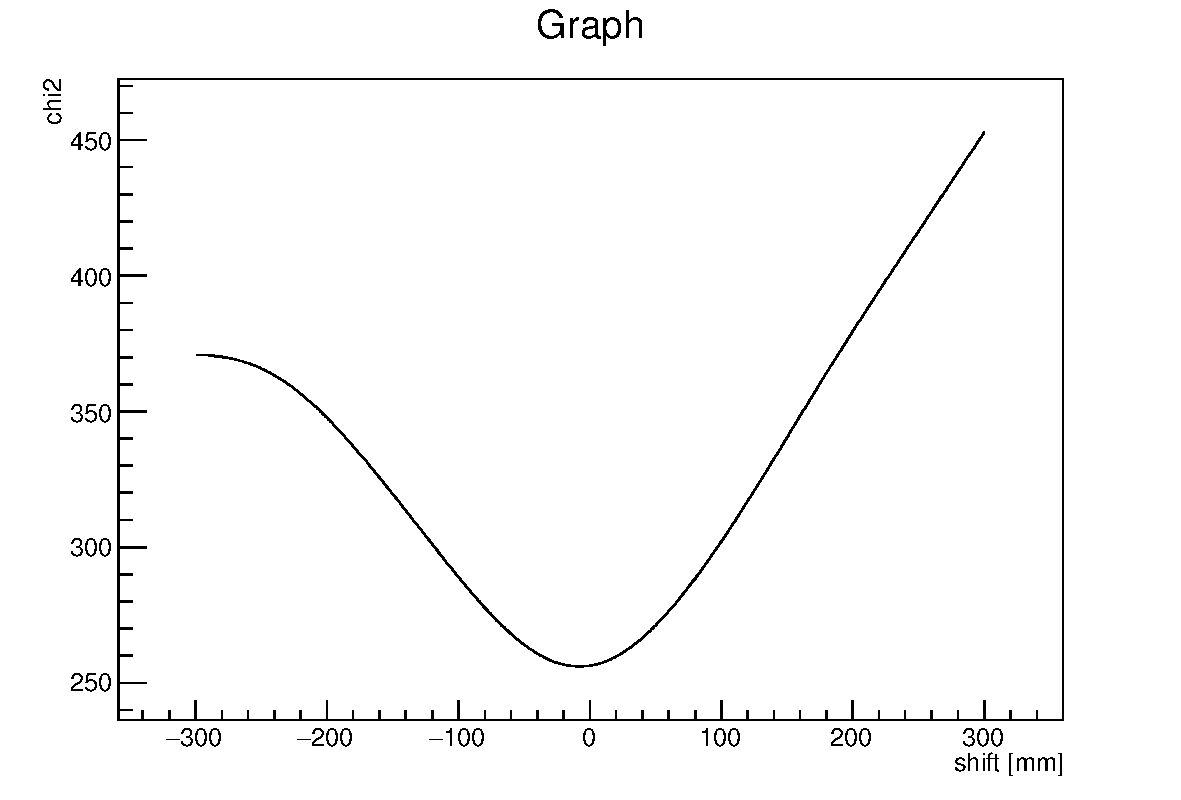
\includegraphics[width=0.33\textwidth]{./Figure/2017-08-02_Distribution_Chi2_1e8_LC.pdf}}
  %\subfloat[\label{fig:fig_Results_Chi2_Distribution_Variation_CC_simulation_Hadronth_LC}]{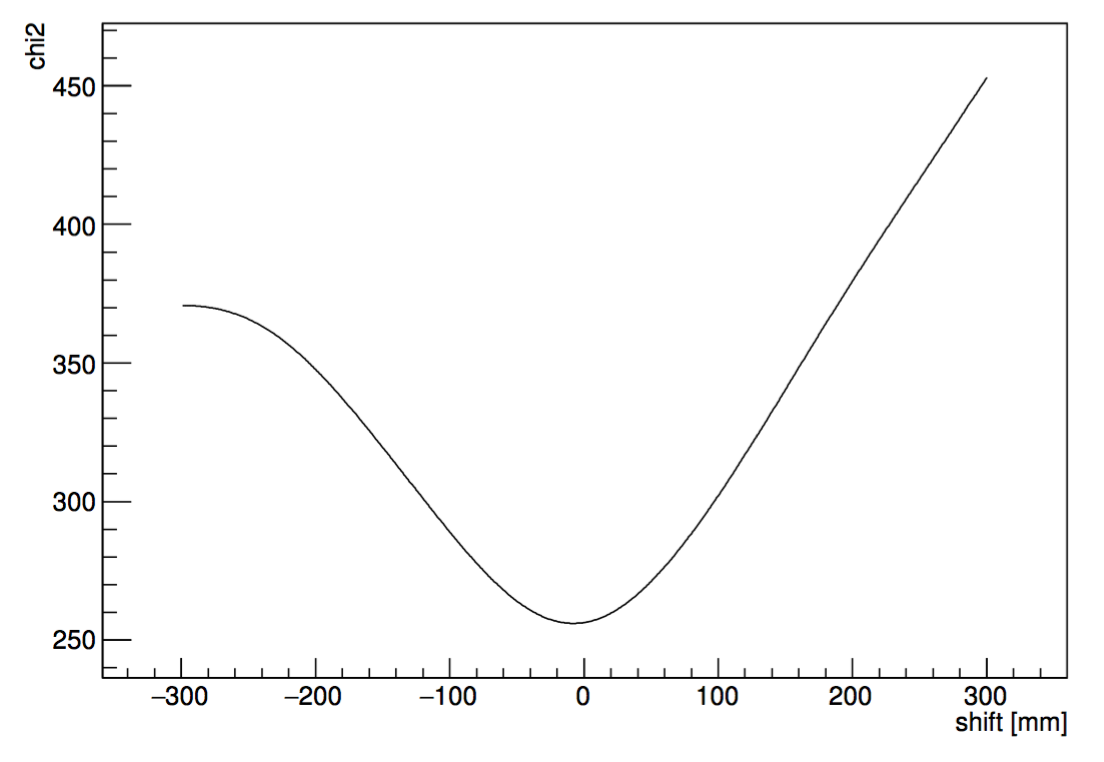
\includegraphics[width=0.45\textwidth]{./Figure/chi2_linecone.png}}
  % \subfloat[\label{fig:fig_Results_Chi2_Distribution_Variation_CC_simulation_Hadronth_MLEM}]{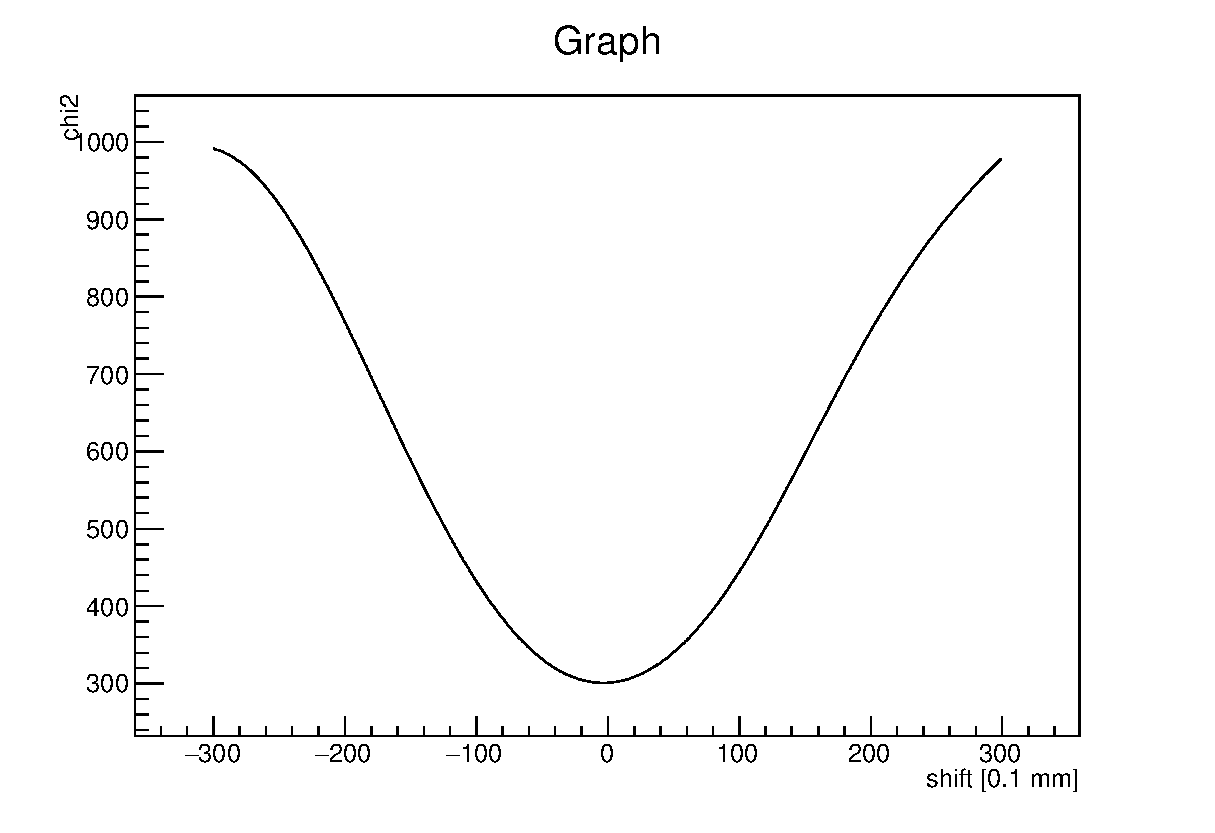
\includegraphics[width=0.33\textwidth]{./Figure/2017-08-02_Distribution_Chi2_Results_binning_1mm_ShiftNurbs0_1mm_1e8_article_MLEM.eps}}\\
  %\subfloat[\label{fig:fig_Results_Chi2_Distribution_Variation_CC_simulation_Hadronth_MLEM}]{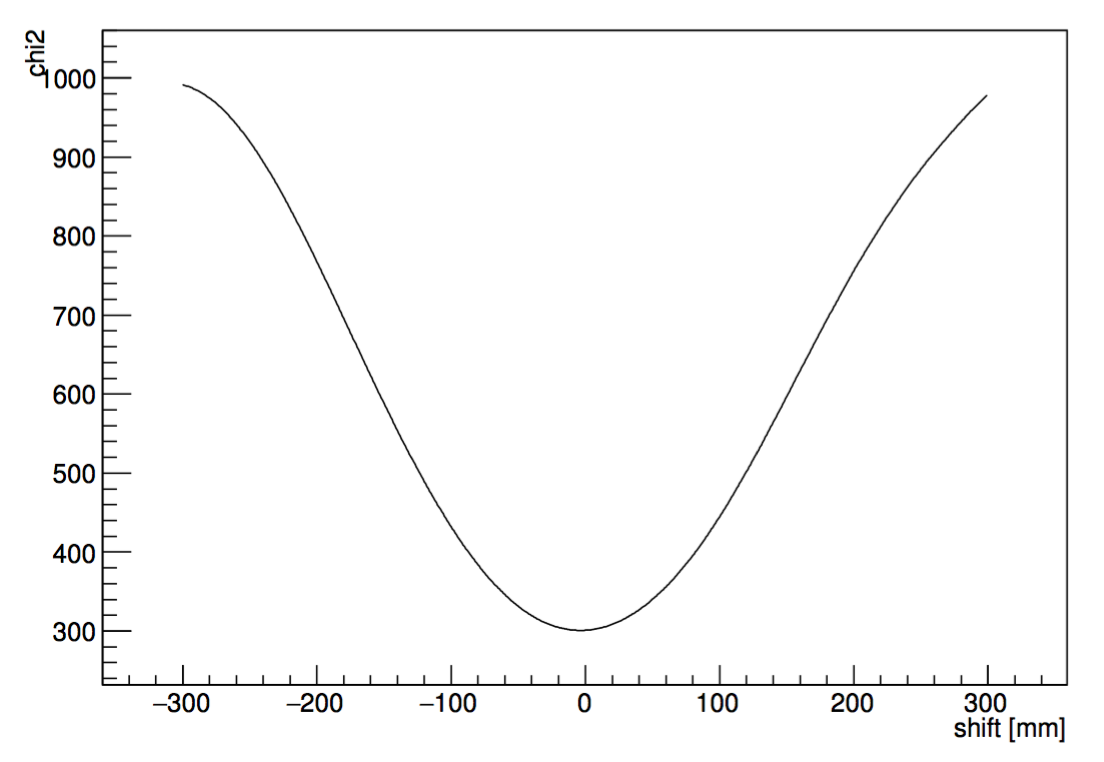
\includegraphics[width=0.45\textwidth]{./Figure/chi2_MLEM.png}}\\
  % \subfloat[\label{fig:fig_Results_Precision_Distribution_Variation_CC_simulation_Hadronth_LC} ]{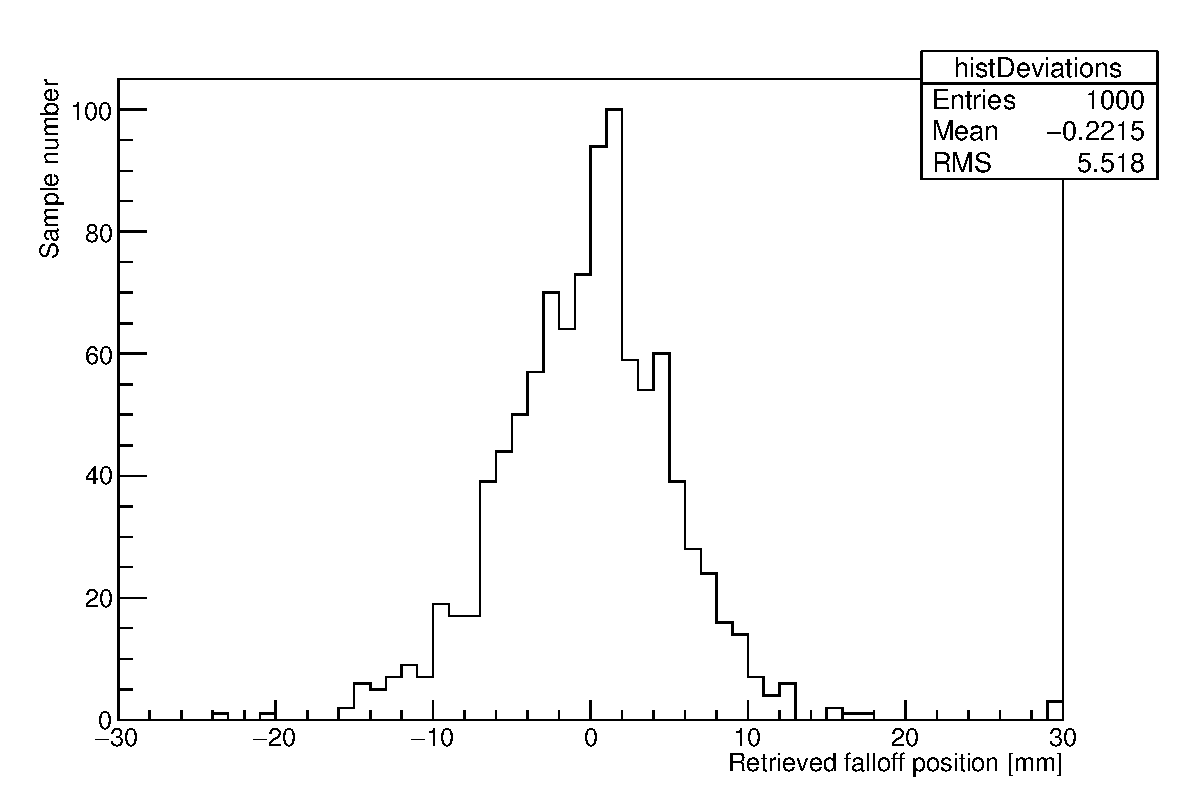
\includegraphics[width=0.33\textwidth]{./Figure/2017-08-02_Distribution_finale_1e8_Article_LC.pdf}}
  \subfloat[\label{fig:fig_Results_Precision_Distribution_Variation_CC_simulation_Hadronth_LC} ]{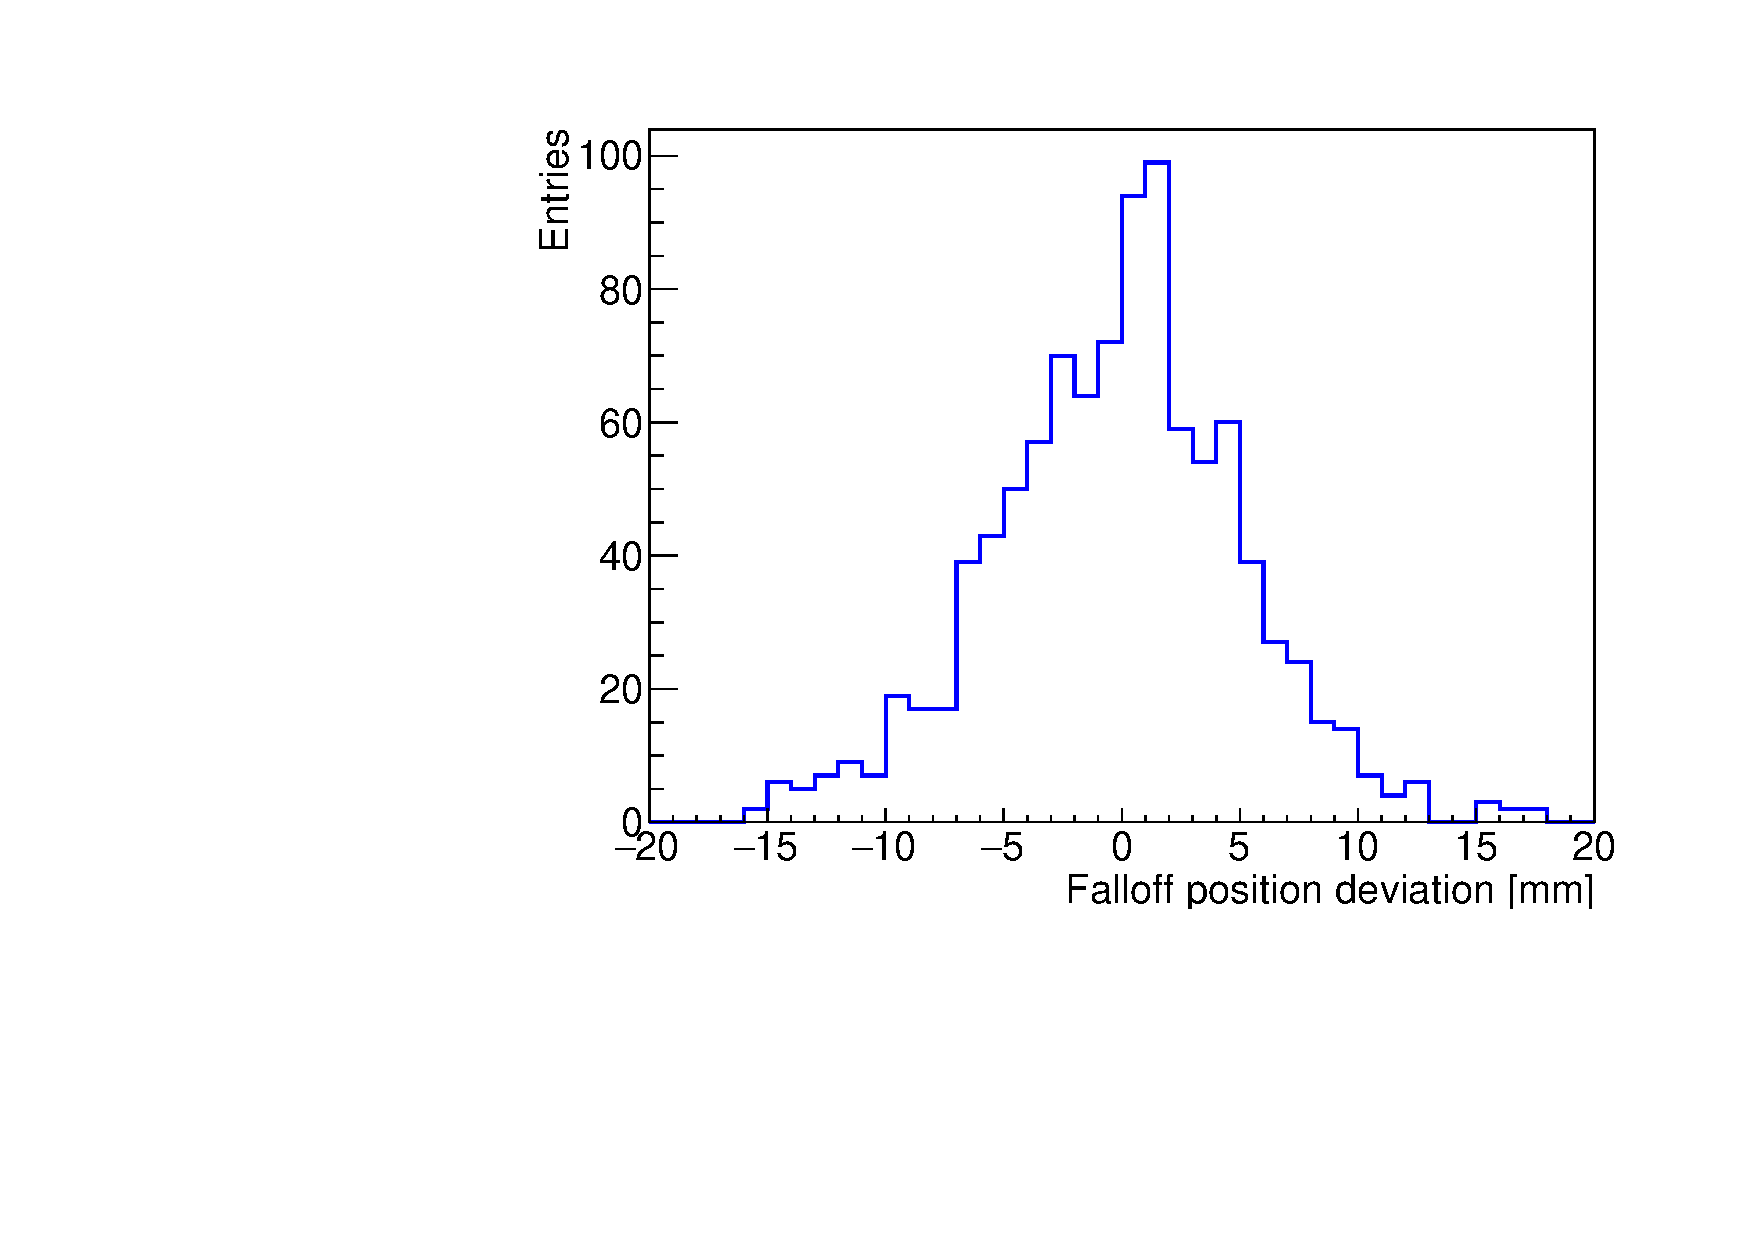
\includegraphics[width=0.48\textwidth]{./Figure/new/LC_histo_deviations.pdf}}
  %{./Figure/deviation_linecone.png}}
  % \subfloat[\label{fig:fig_Results_Precision_Distribution_Variation_CC_simulation_Hadronth_MLEM} ]{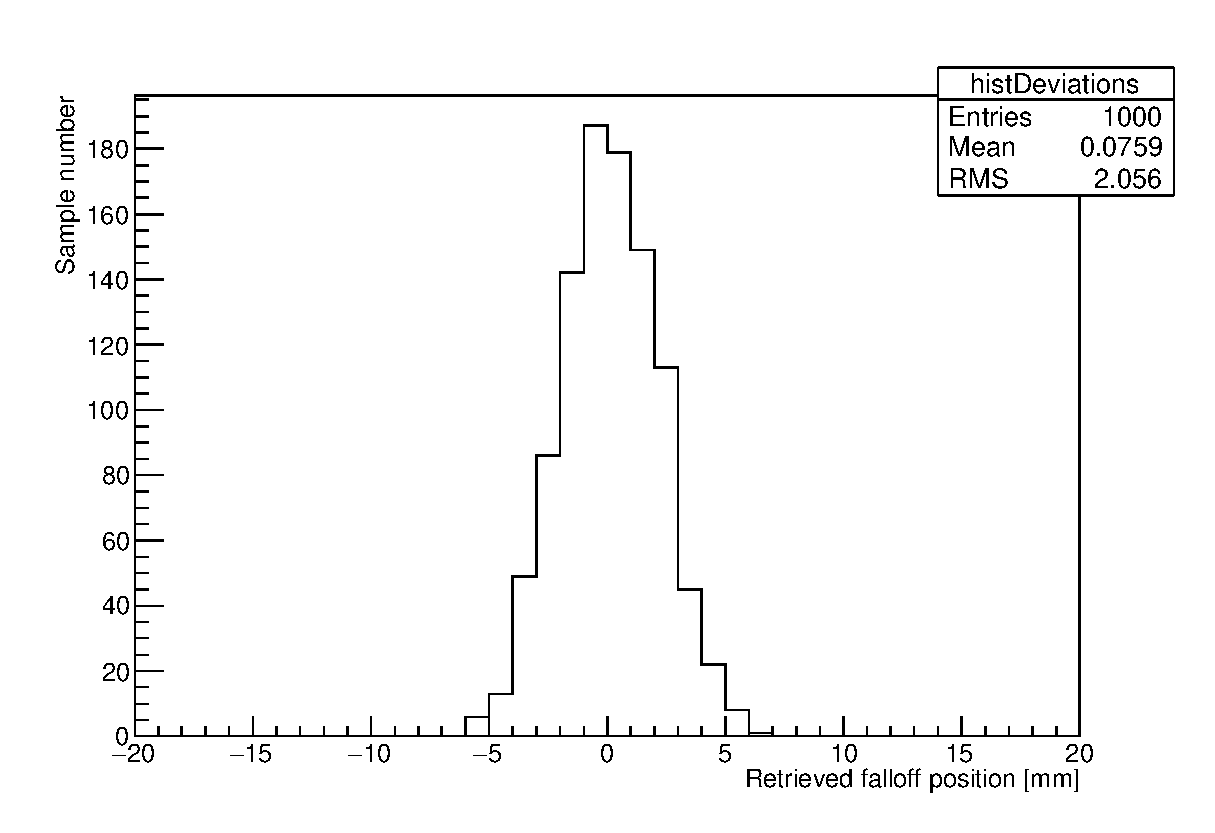
\includegraphics[width=0.33\textwidth]{./Figure/2017-08-02_FallOff_Results_binning_1mm_ShiftNurbs0_1mm_1e8_Article_MLEM.eps}}
  \subfloat[\label{fig:fig_Results_Precision_Distribution_Variation_CC_simulation_Hadronth_MLEM} ]{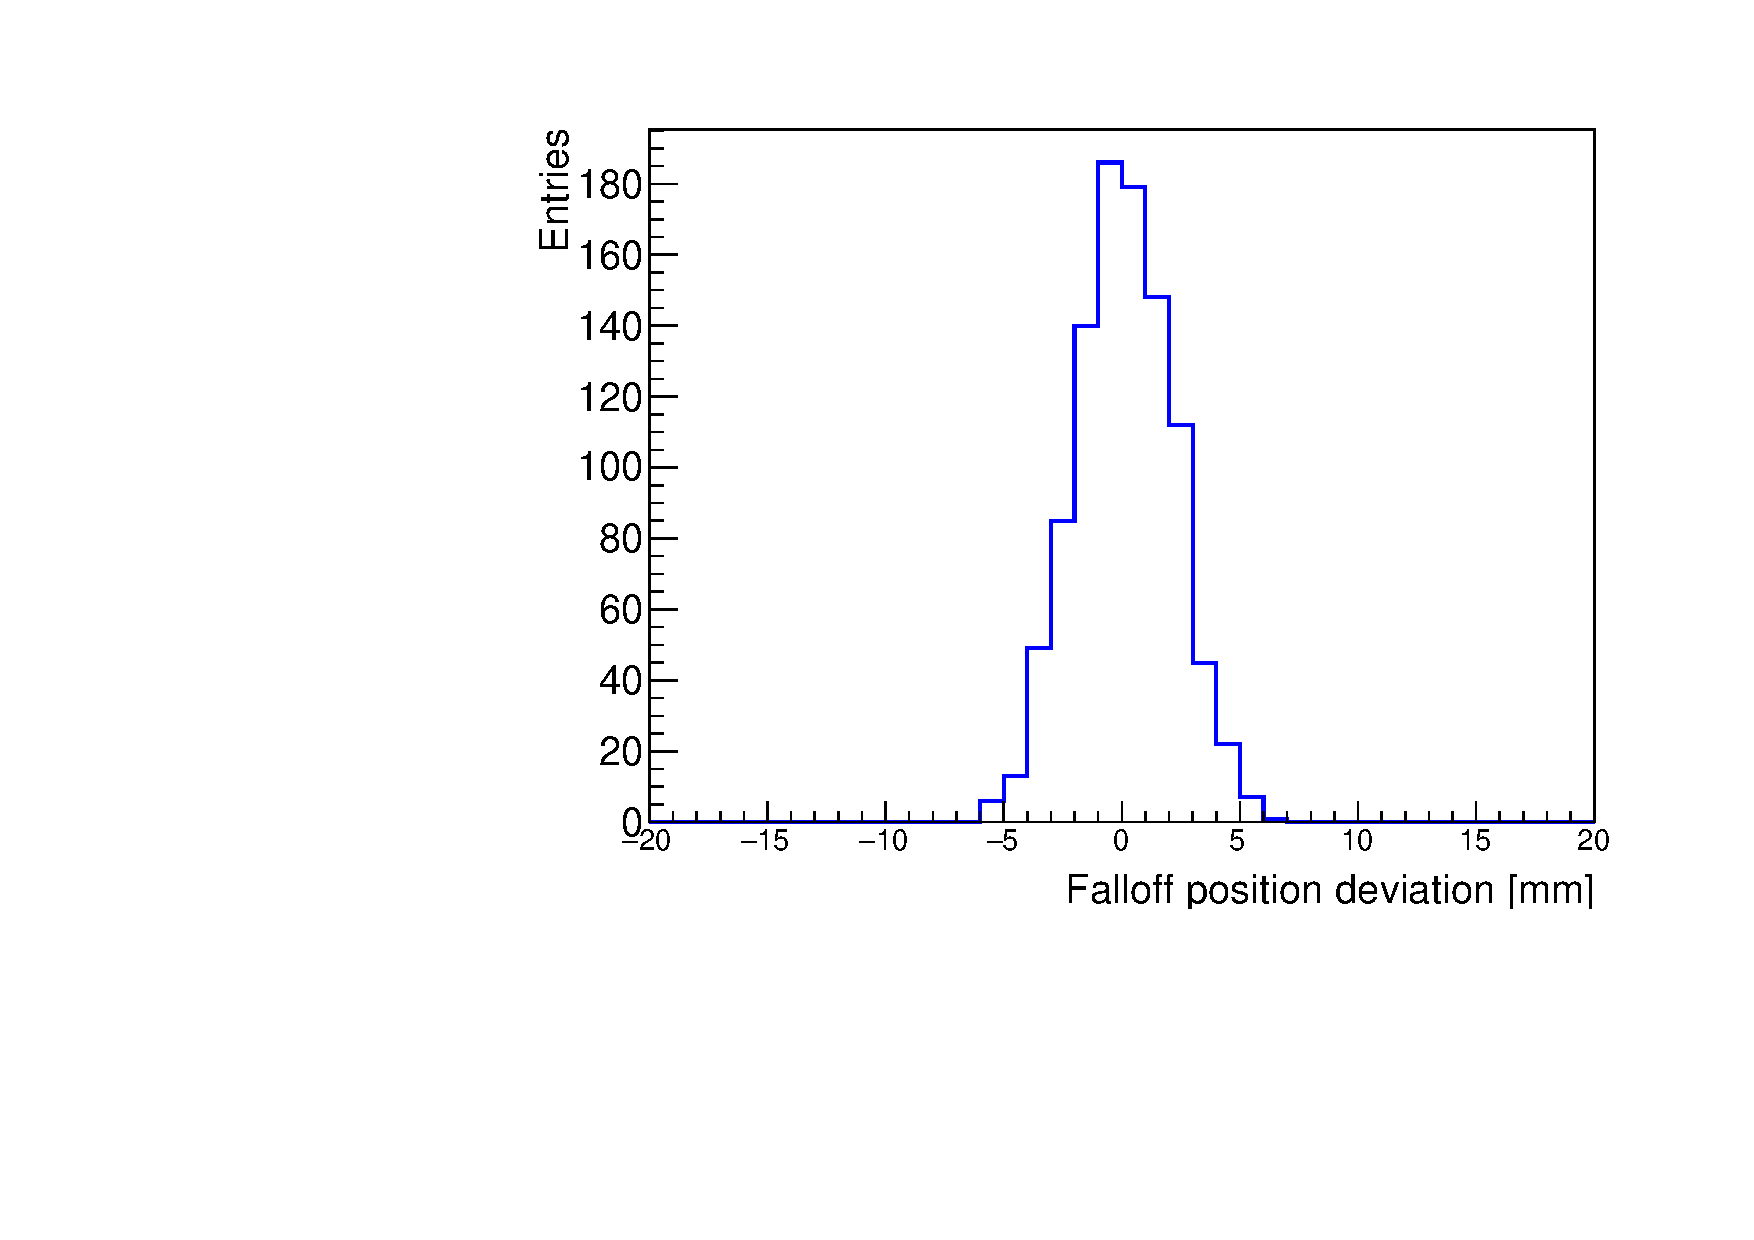
\includegraphics[width=0.48\textwidth]{./Figure/new/MLEM_histo_deviations.pdf}}
  %{./Figure/deviation_MLEM.png}}
  \caption{Distributions of the falloff position deviation with respect to the falloff position of the high statistics reference profile for 1000 realizations with 10$^8$ primary protons, obtained with line-cone (a) and MLEM (b) reconstruction. The RMS of these distributions represents the Compton camera precision for the selected statistics.}\end{figure}

\begin{figure}
\centering
\subfloat[]{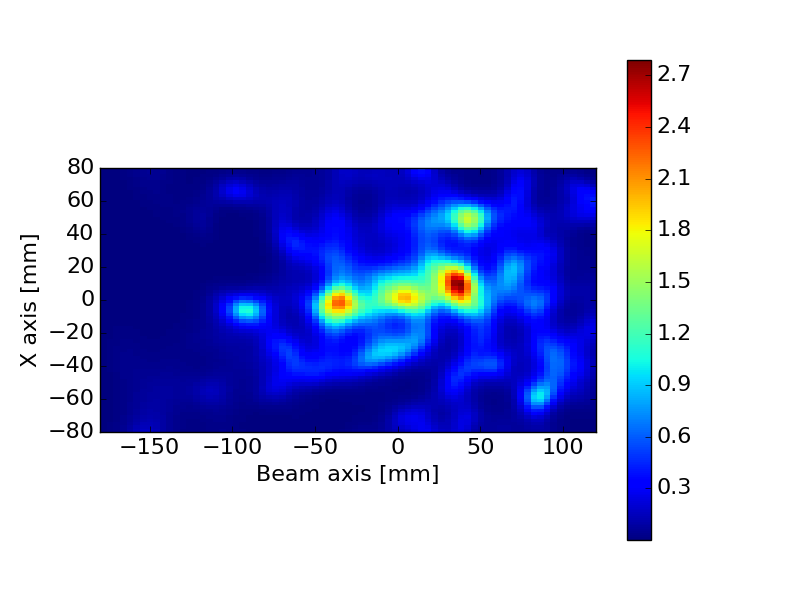
\includegraphics[width=0.5\textwidth,clip=true,trim=0 70 130 90]{./Figure/projection2D_Z_corr_r20.png}}
\subfloat[]{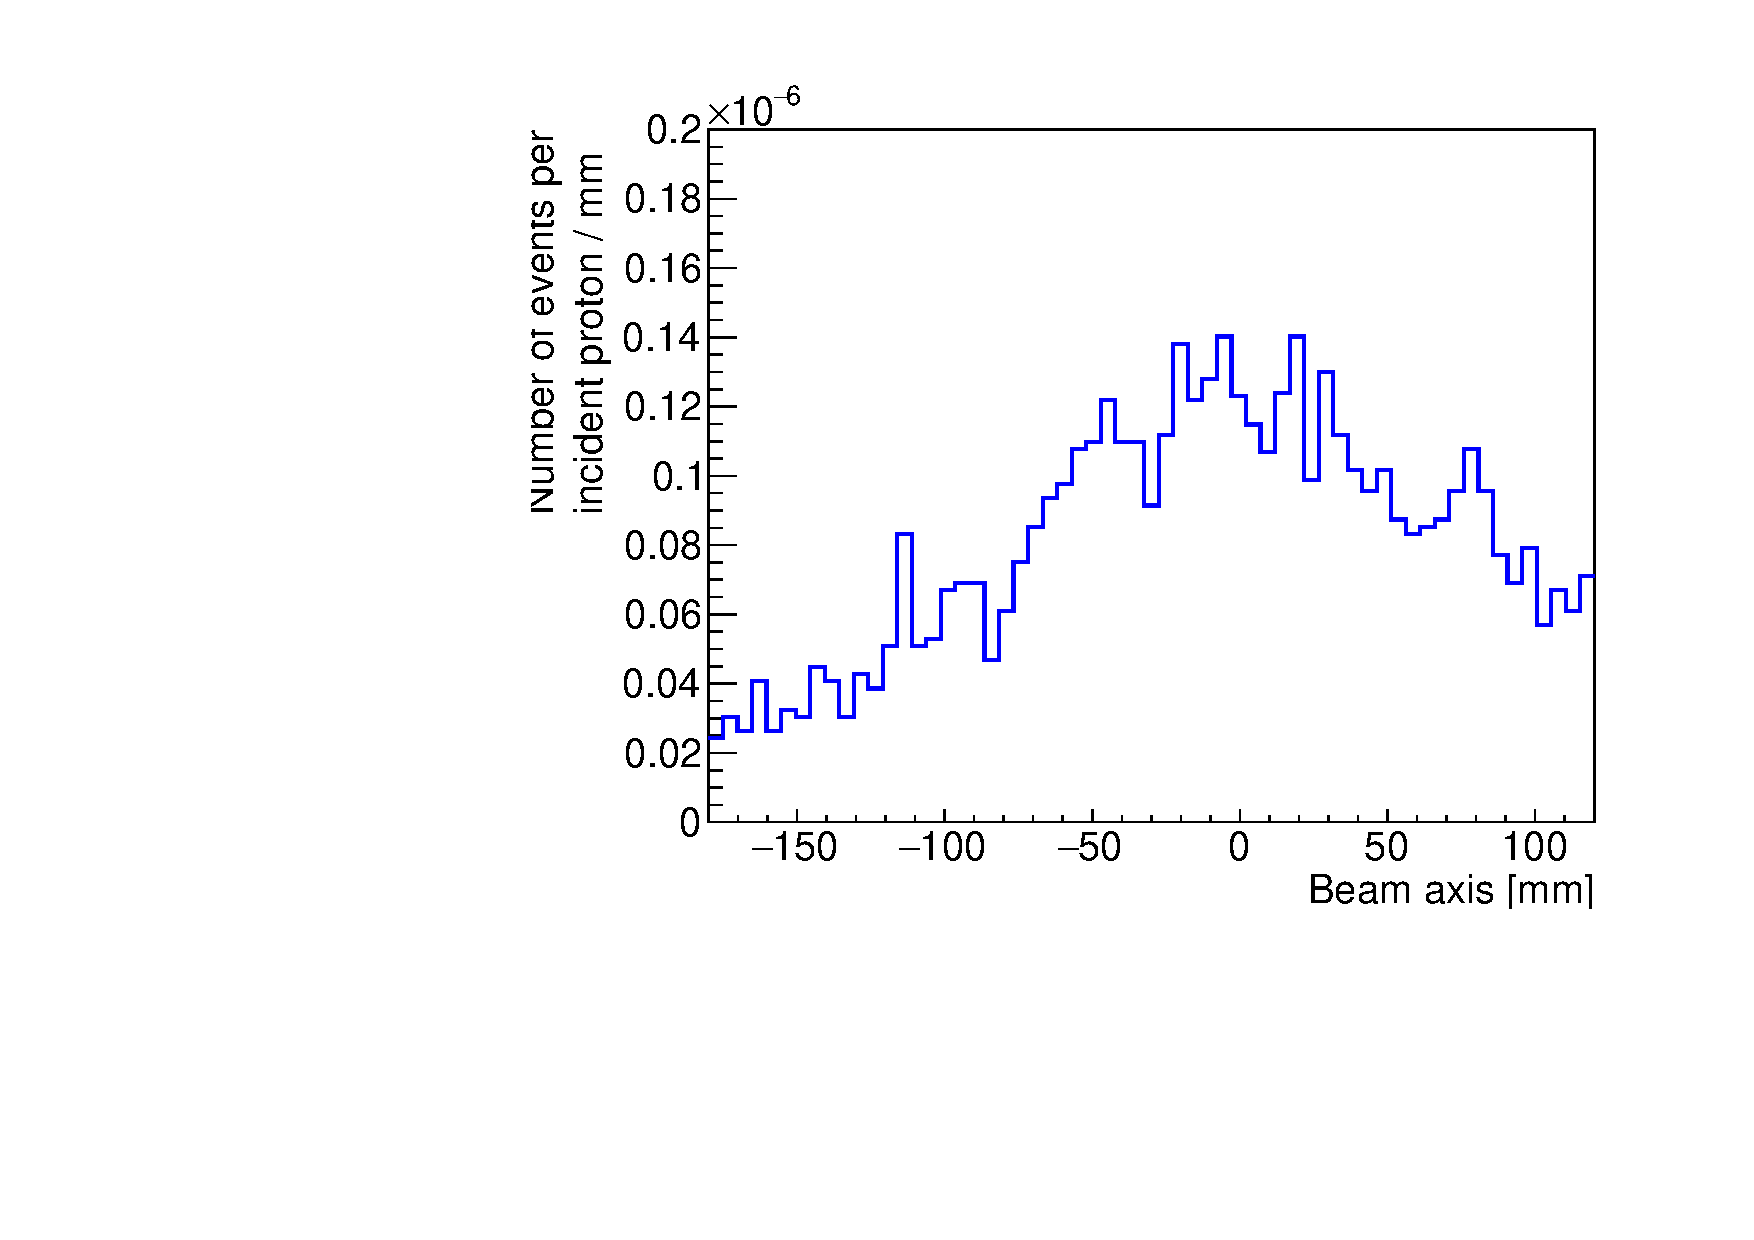
\includegraphics[width=0.5\textwidth]{./Figure/new/recon_profile_line-cone_lowStat_norm.pdf}}\\
%\subfloat[]{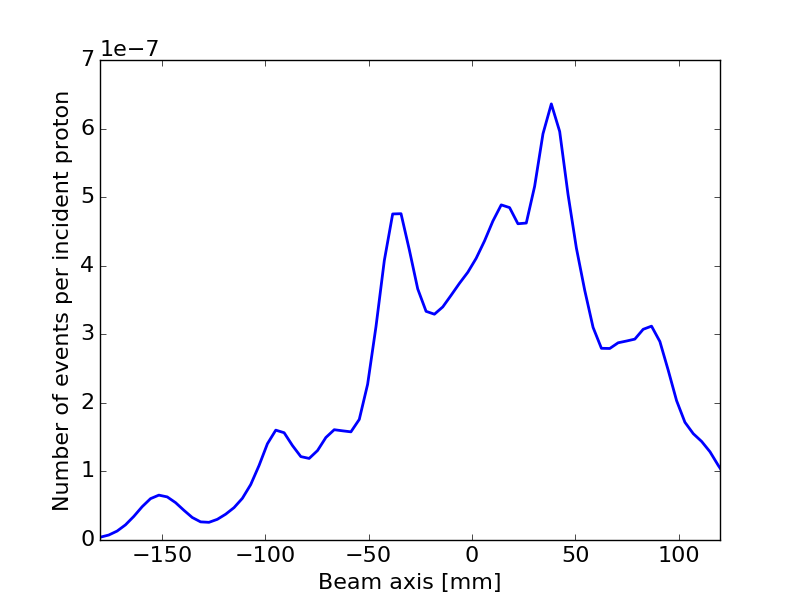
\includegraphics[width=0.5\textwidth]{./Figure/profileY_corr_r20.png}}\\
\subfloat[]{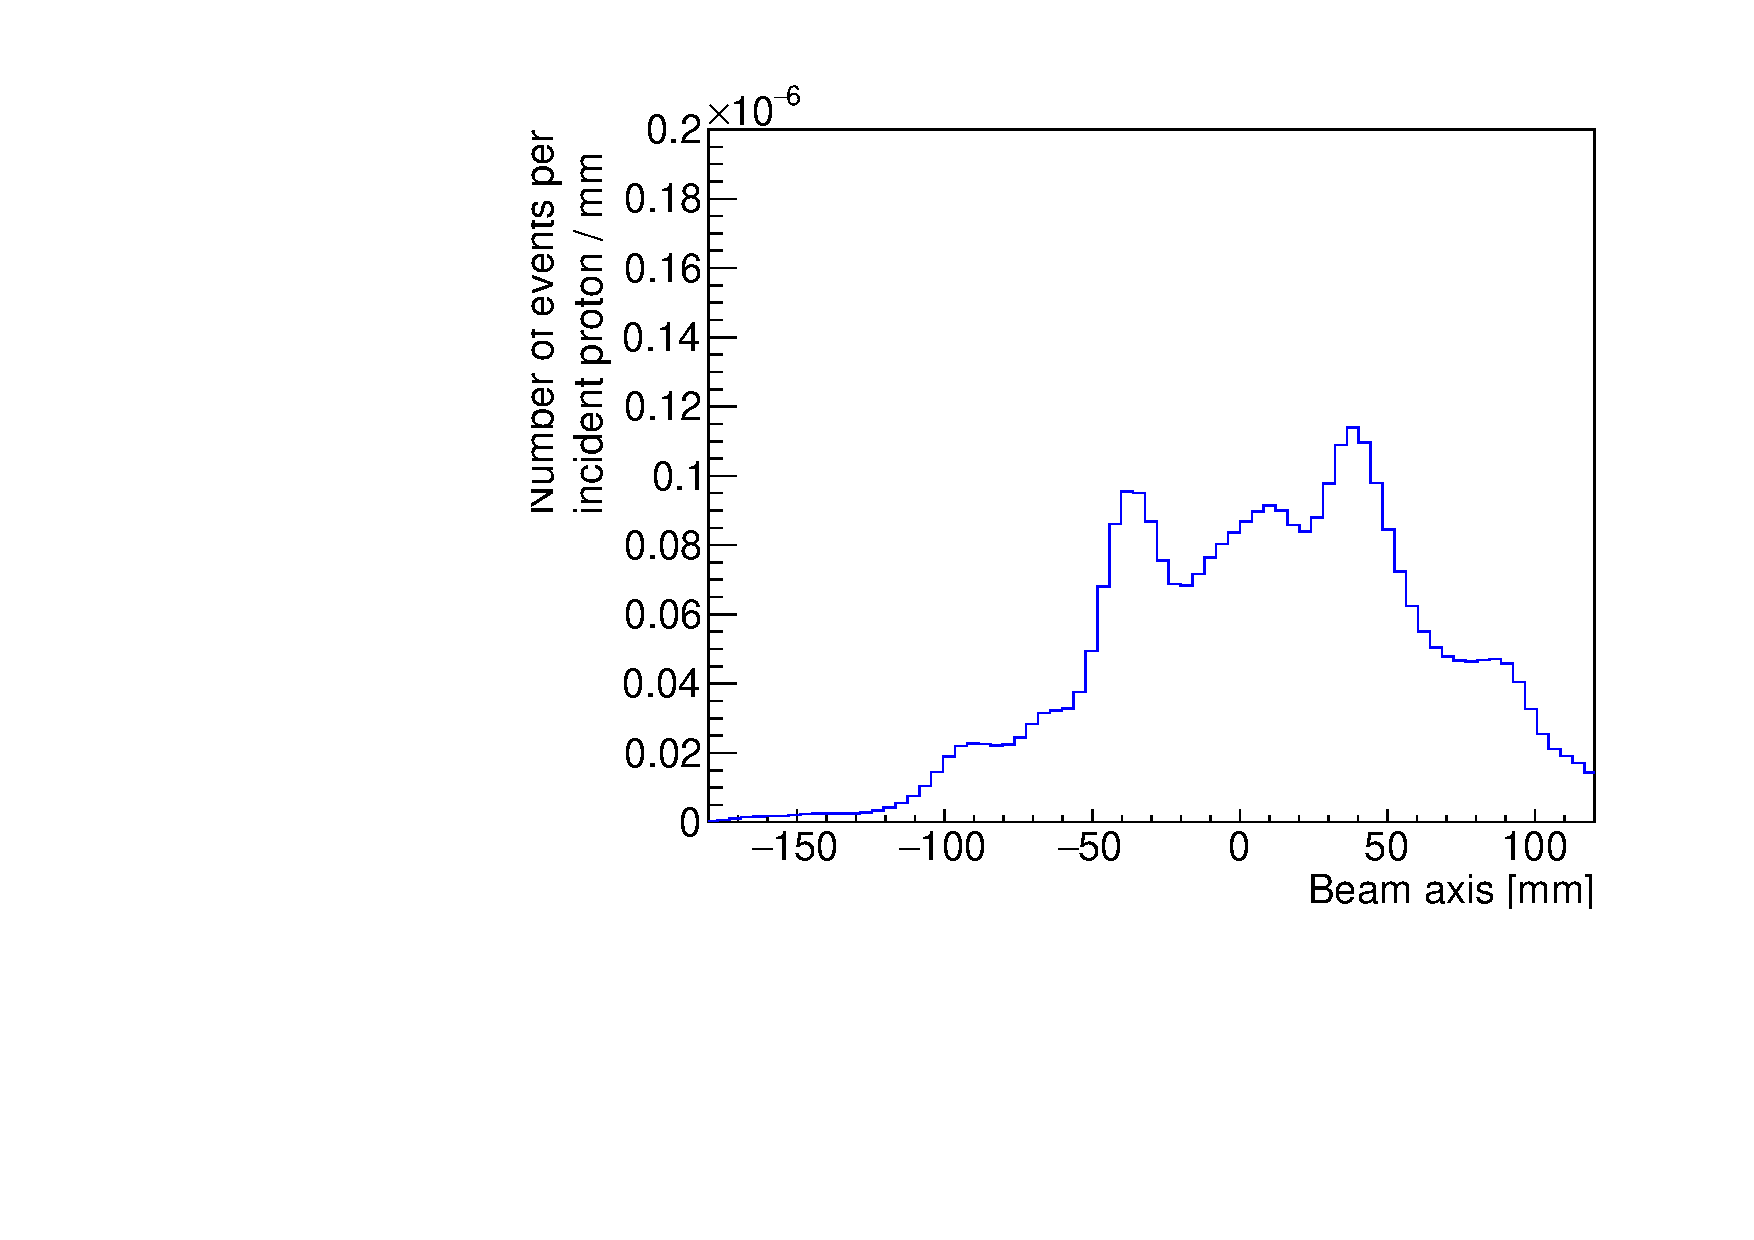
\includegraphics[width=0.5\textwidth]{./Figure/new/reconstructed_lowStat_profile_norm.pdf}}
%\subfloat[]{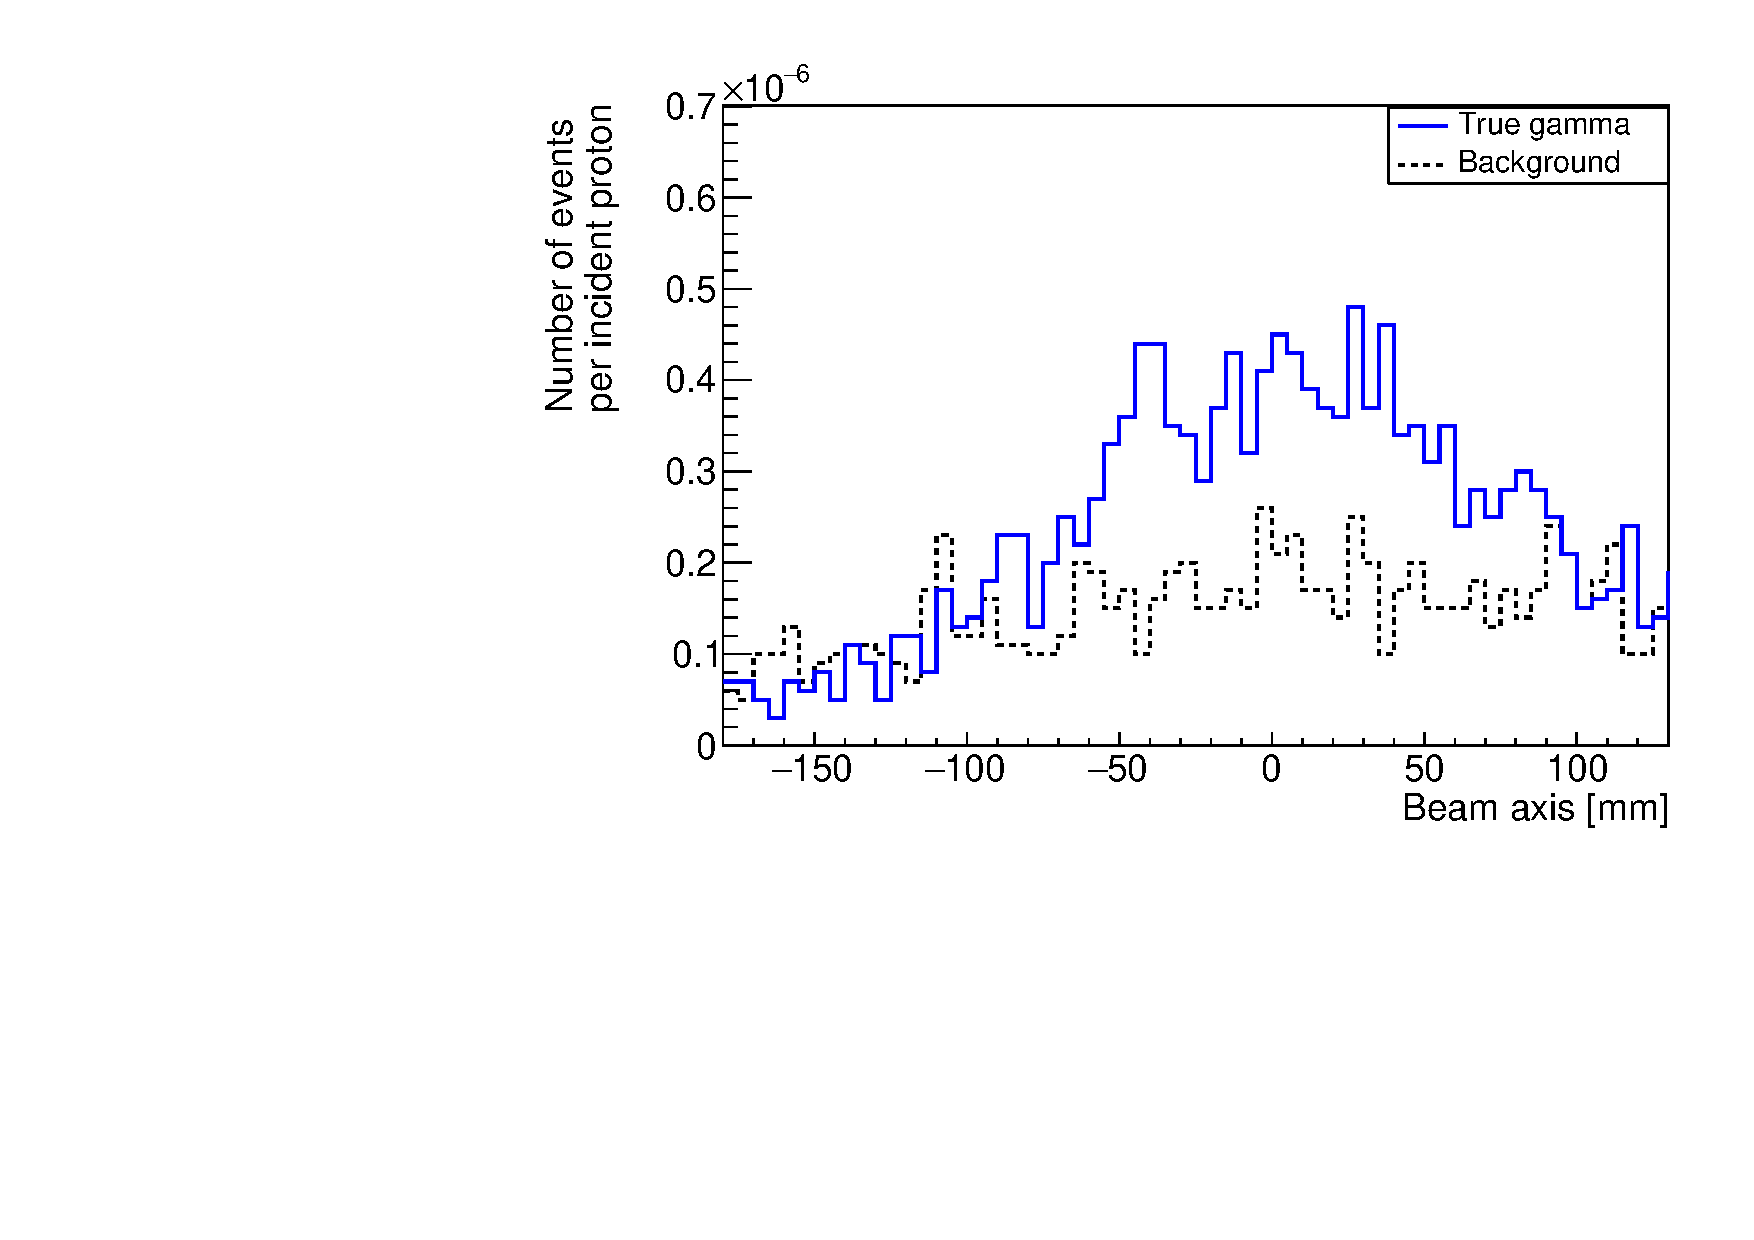
\includegraphics[width=0.5\textwidth]{./Figure/2015_02_16_Reconstruction_coinc_160MeVProton_TOF_6ns_file0to100_zoom.pdf}}
\caption{Line-cone and LM-MLEM reconstruction for a 160~MeV proton beam, $10^{8}$ total incident protons. The beam intensity is 1 proton per bunch. The Compton camera is centered at the expected Bragg peak position, $y=+50\,$mm. The time-of-flight event selection is applied on the collected data set. 20 iterations are performed for the MLEM reconstruction.
Figure (a) represents the MLEM reconstructed 2D image in the plane $(x,y)$, parallel to the camera entrance surface. The position $x=0\,$mm corresponds to the center of the PMMA phantom and the $y$ direction corresponds to the beam axis, with the target entrance at $y=-100\,$mm and the target end at $y=+100\,$mm.  In figure (b) the 1D profile along the $y$ axis is sketched. The profile fall-off is located at $y=+50\,$mm. Figure (c) shows the profile obtained by means of the line-cone algorithm for the same time-of-flight selected data.}
\label{fig:comparison}
\end{figure}

\begin{figure}
\centering
\subfloat[]{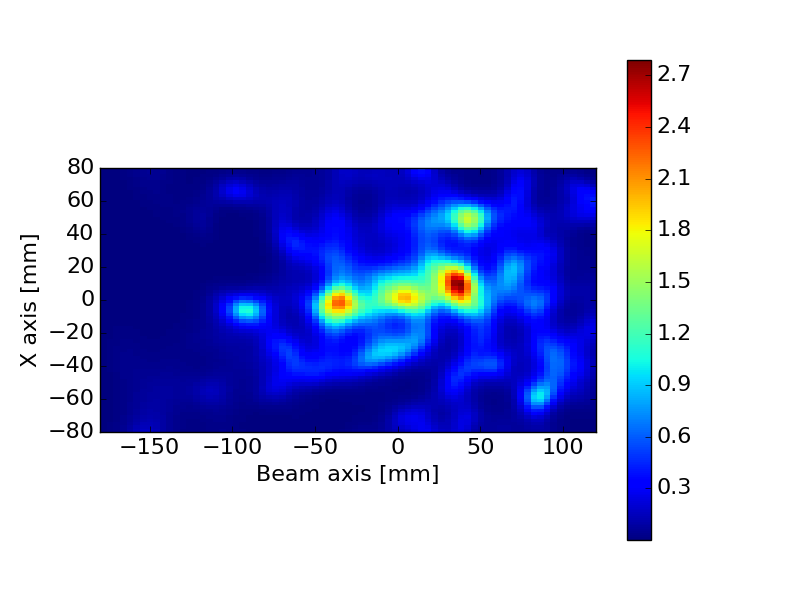
\includegraphics[width=0.5\textwidth,clip=true,trim=0 70 130 90]{./Figure/projection2D_Z_corr_r20.png}}
\subfloat[]{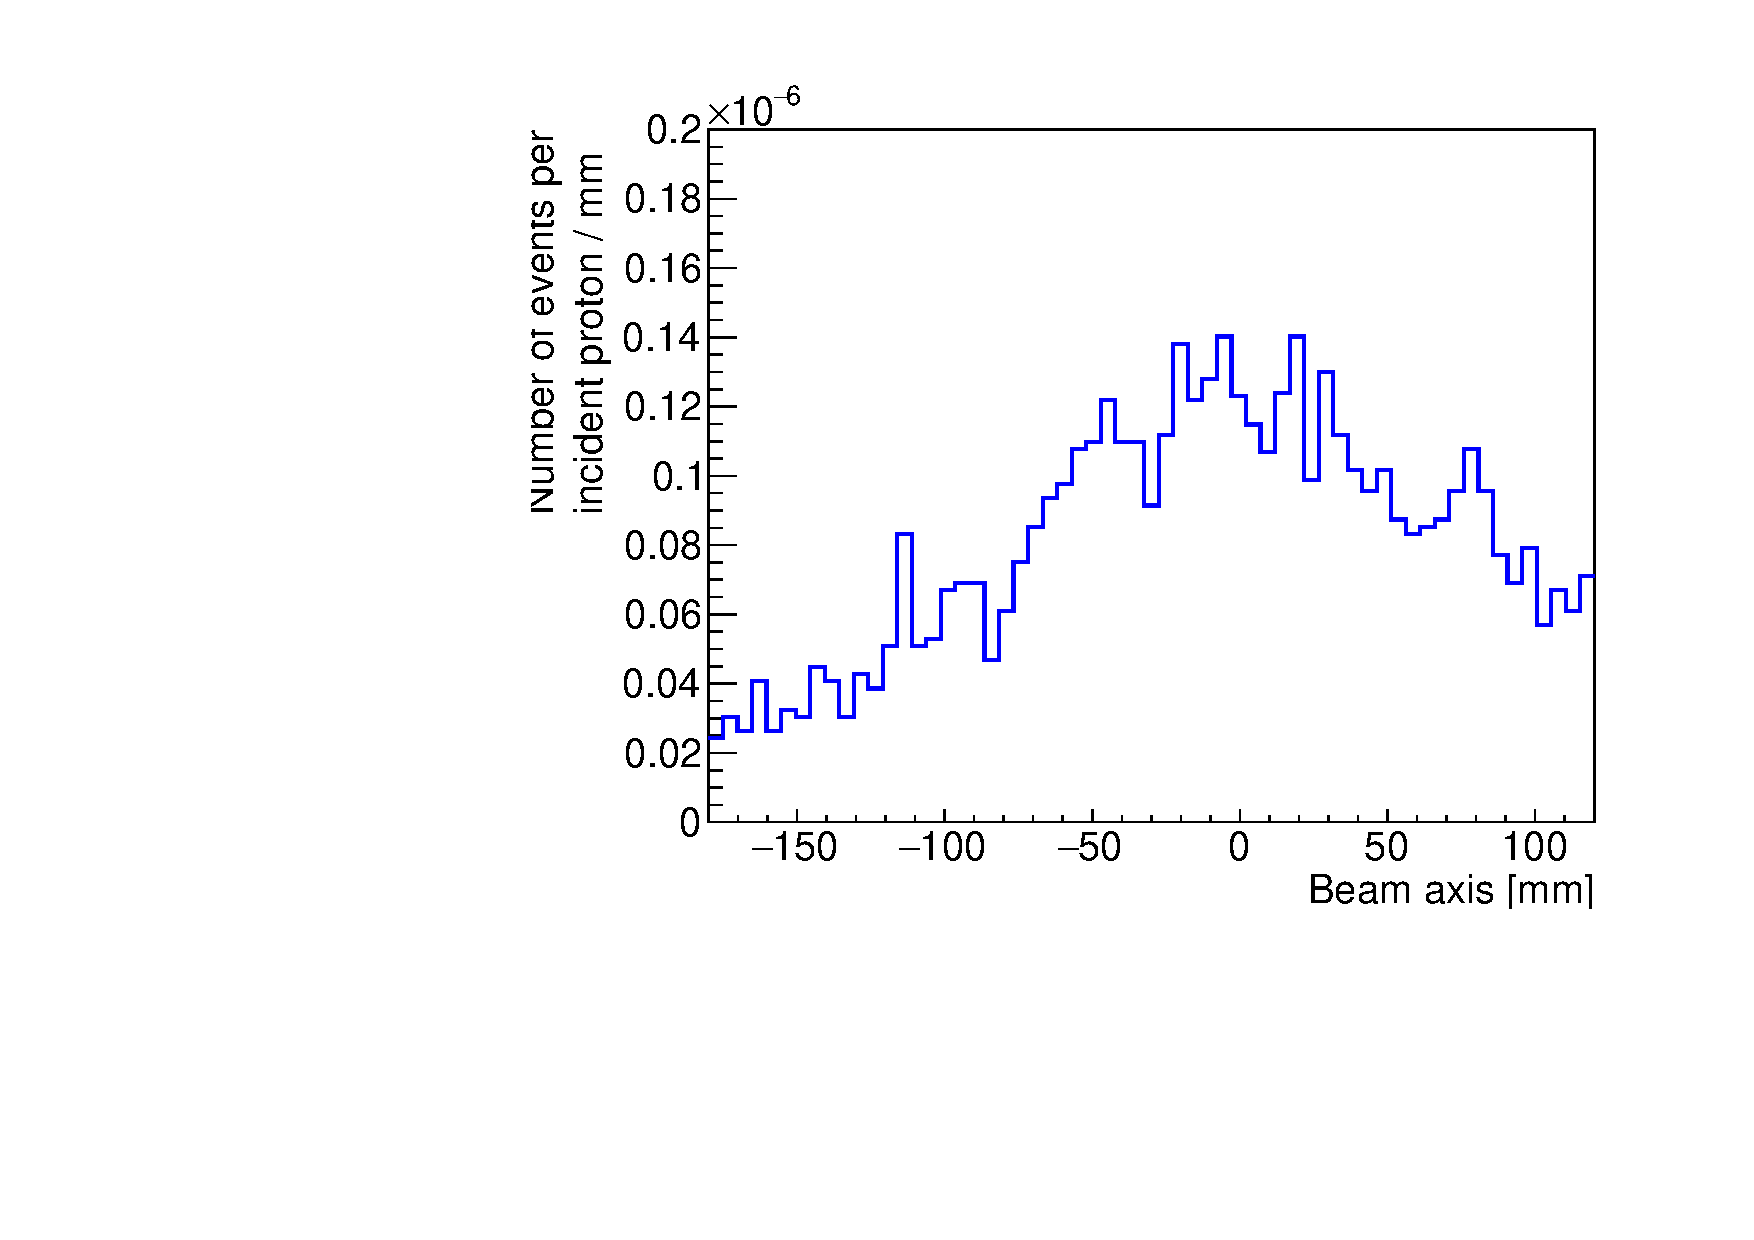
\includegraphics[width=0.5\textwidth]{./Figure/new/recon_profile_line-cone_lowStat_norm.pdf}}\\
%\subfloat[]{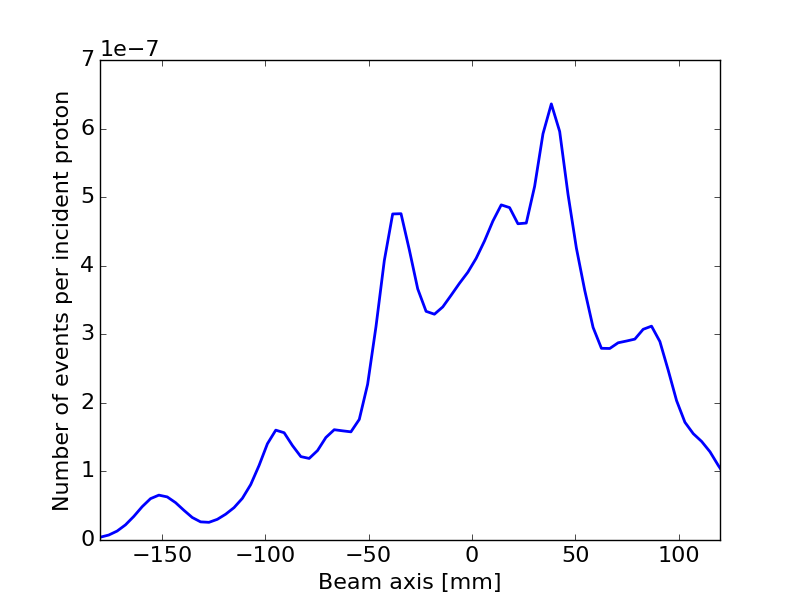
\includegraphics[width=0.5\textwidth]{./Figure/profileY_corr_r20.png}}\\
\subfloat[]{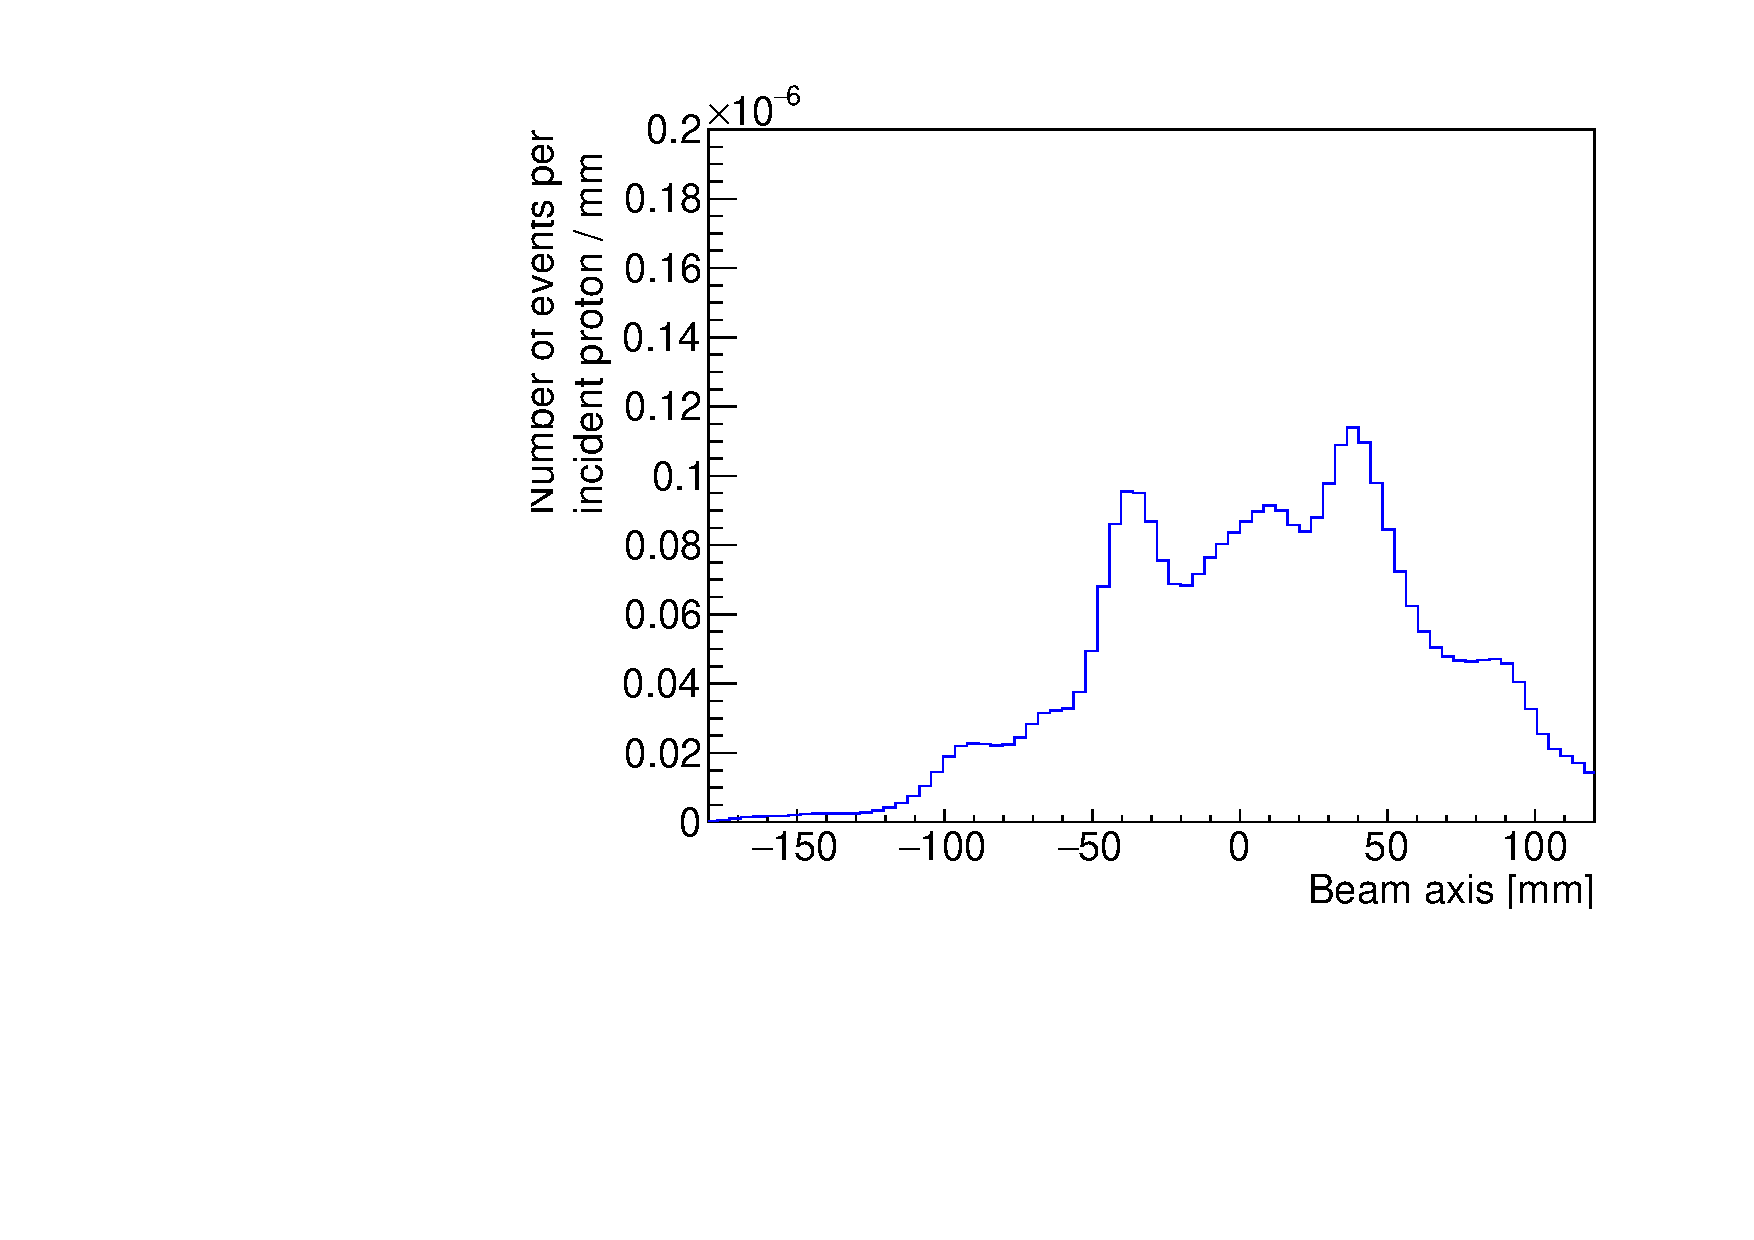
\includegraphics[width=0.5\textwidth]{./Figure/new/reconstructed_lowStat_profile_norm.pdf}}
%\subfloat[]{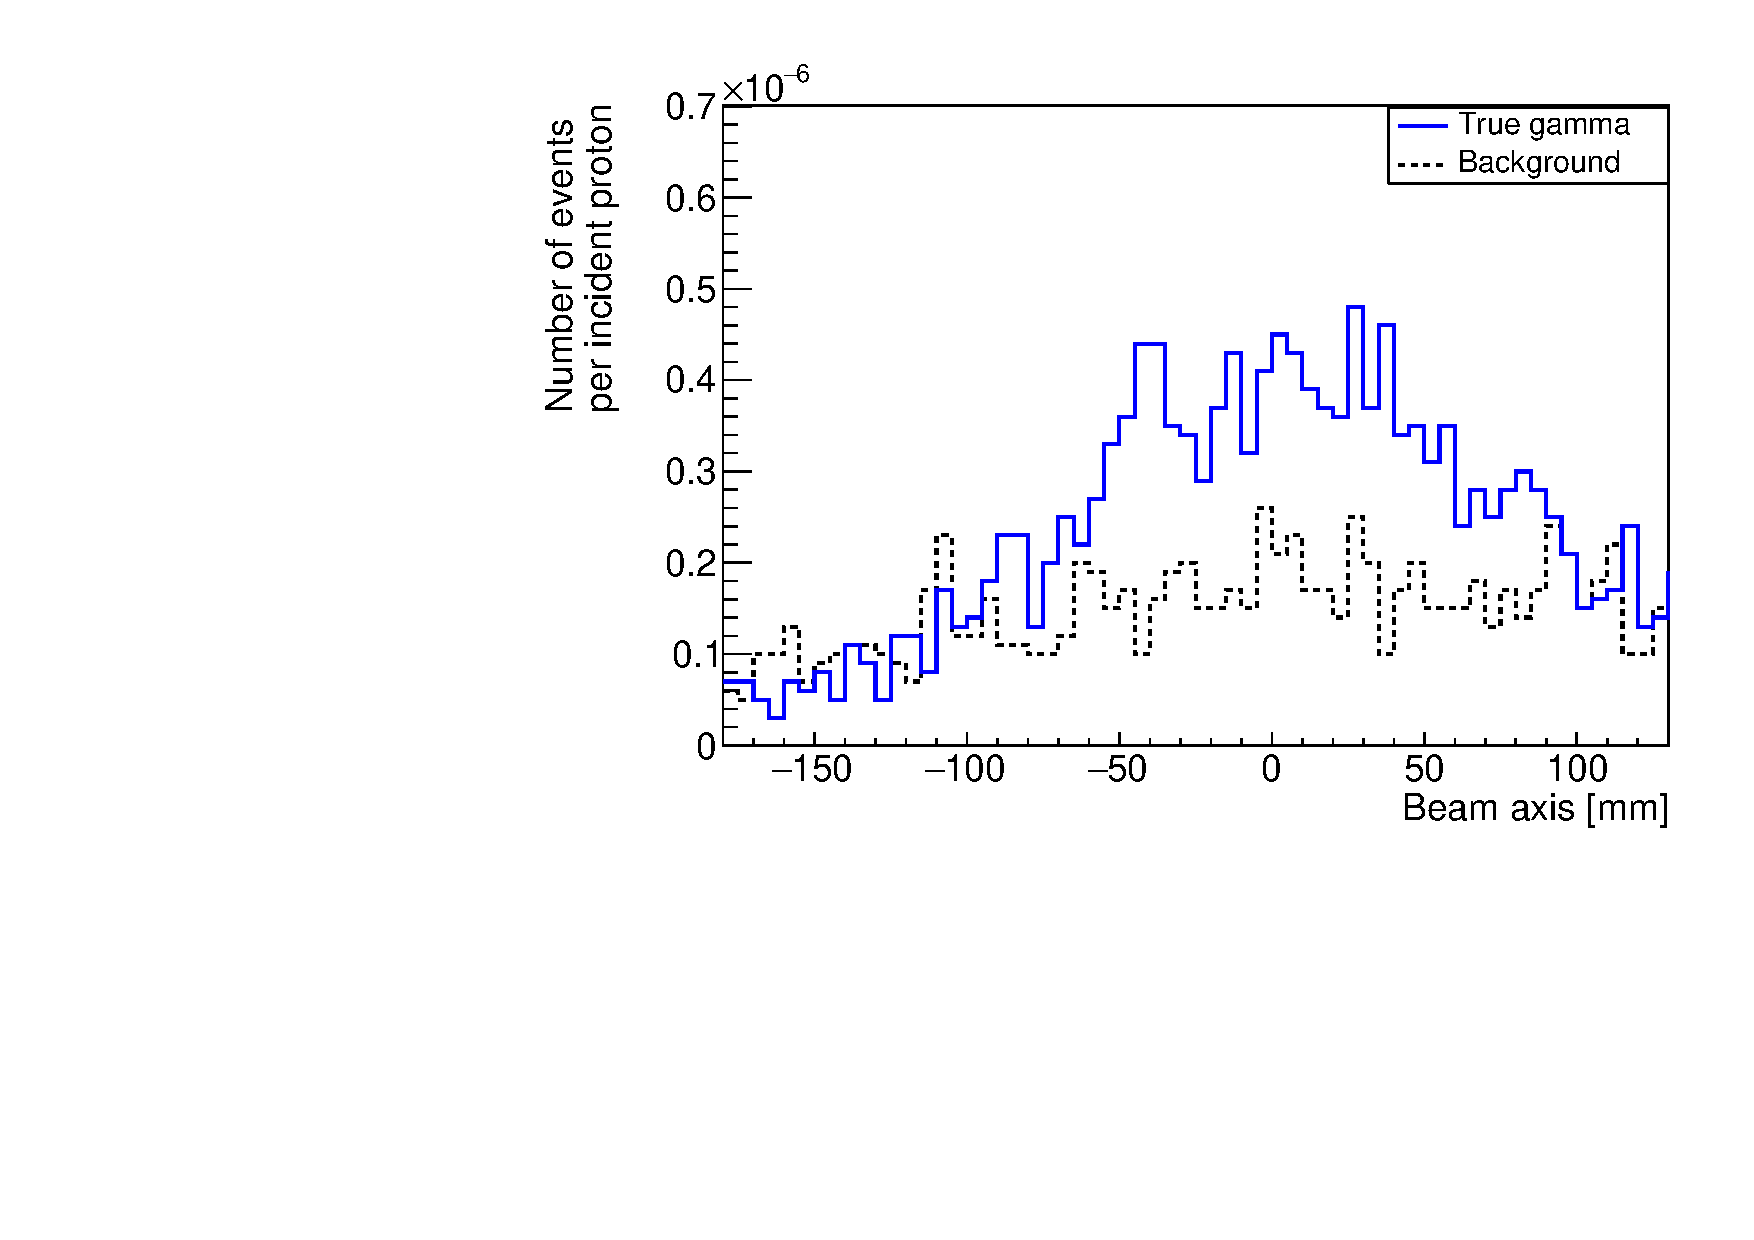
\includegraphics[width=0.5\textwidth]{./Figure/2015_02_16_Reconstruction_coinc_160MeVProton_TOF_6ns_file0to100_zoom.pdf}}
\caption{Line-cone and LM-MLEM reconstruction for a 160~MeV proton beam, $10^{8}$ total incident protons. The beam intensity is 200 proton per bunch. The Compton camera is centered at the expected Bragg peak position, $y=+50\,$mm. The time-of-flight event selection is applied on the collected data set. 20 iterations are performed for the MLEM reconstruction.
Figure (a) represents the MLEM reconstructed 2D image in the plane $(x,y)$, parallel to the camera entrance surface. The position $x=0\,$mm corresponds to the center of the PMMA phantom and the $y$ direction corresponds to the beam axis, with the target entrance at $y=-100\,$mm and the target end at $y=+100\,$mm.  In figure (b) the 1D profile along the $y$ axis is sketched. The profile fall-off is located at $y=+50\,$mm. Figure (c) shows the profile obtained by means of the line-cone algorithm for the same time-of-flight selected data.}
\label{fig:comparison}
\end{figure}


The analysis method described in section~\ref{MatMeth:precision} is applied to the different PG obtained profiles to retrieve the camera precision in the falloff identification. The results are shown in figure~\ref{fig:precision}, where the two reconstruction methods are represented by different markers.

\begin{figure}	
\centering
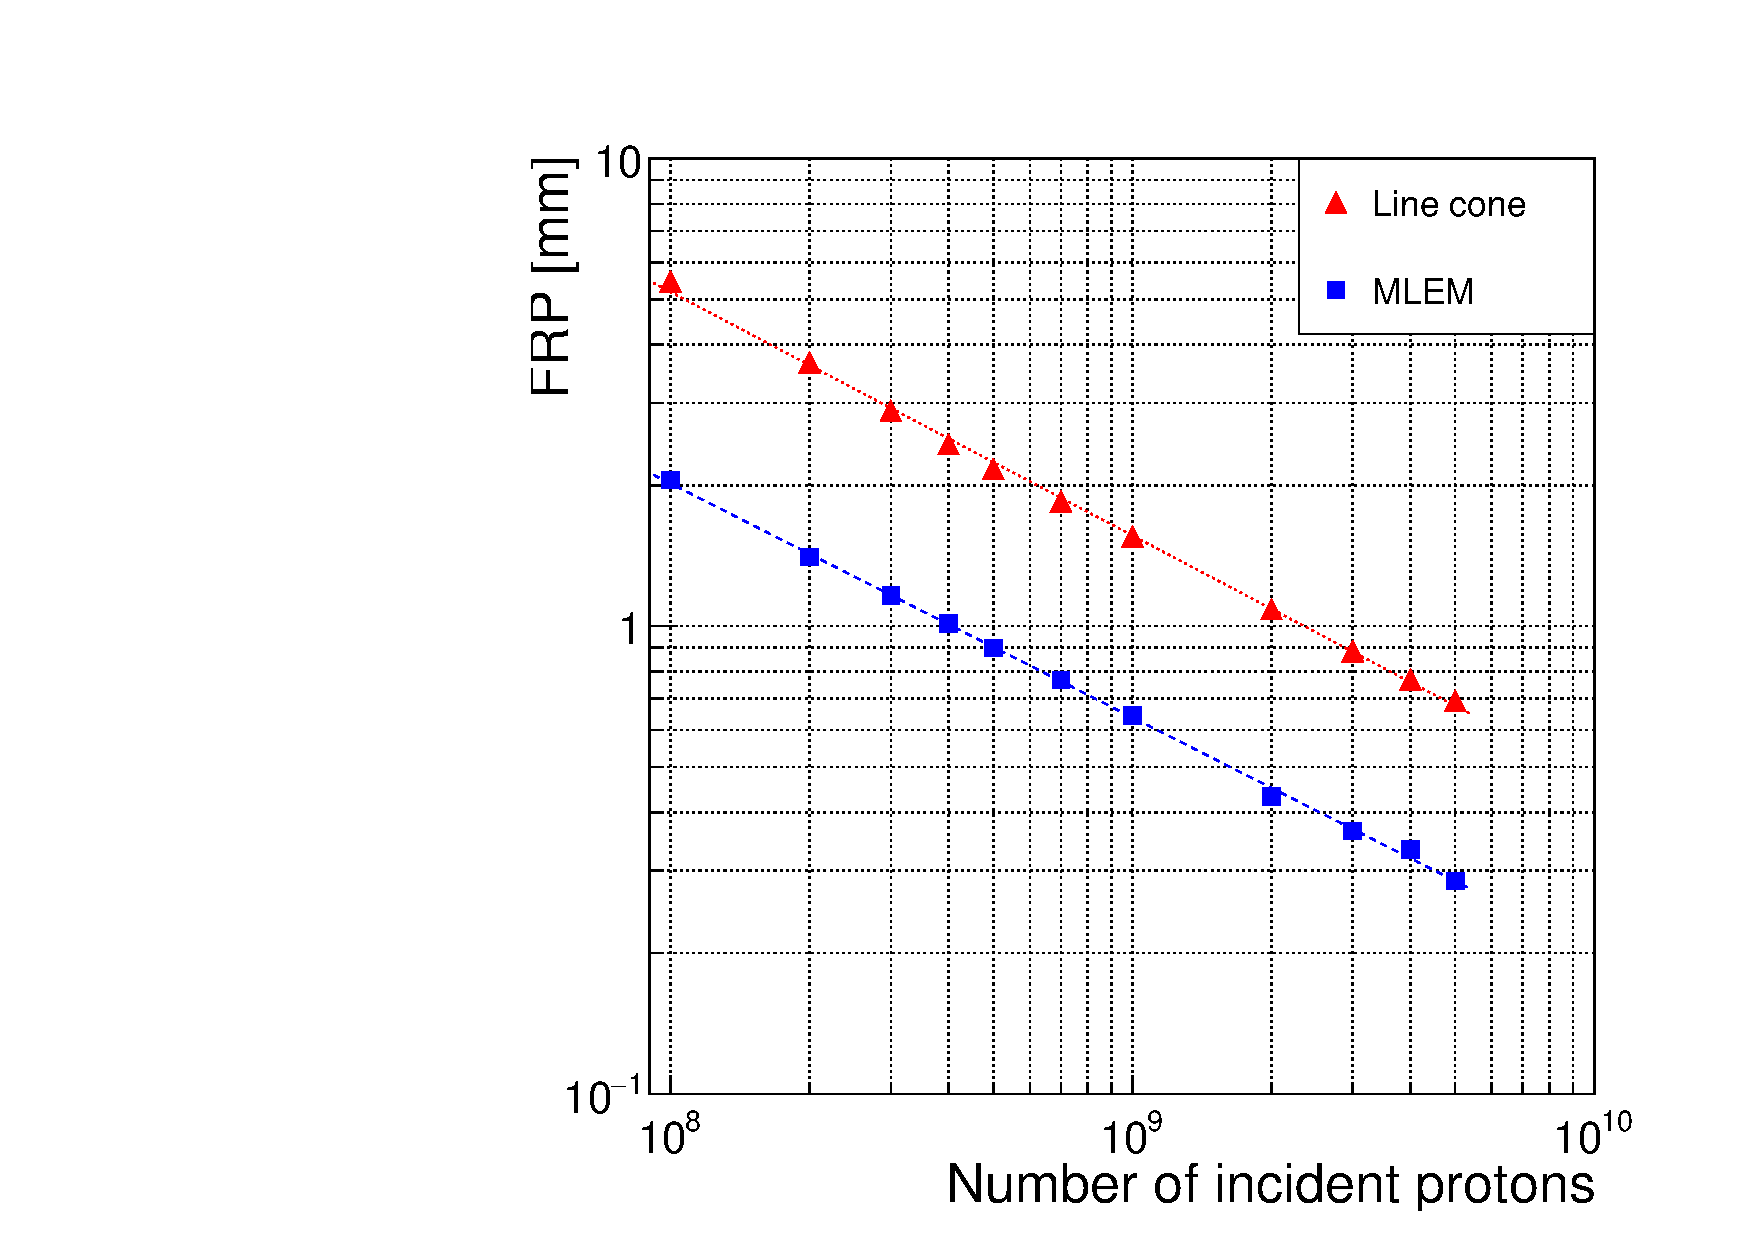
\includegraphics[width=0.7\textwidth]{./Figure/new/precisionVSprimaries.pdf}
%{./Figure/2017-10-21_Precision_Comparaison_linecone_MLEM_Article_Fit.eps}
\caption{Fall-off retrieval precision (FRP) for two different reconstruction algorithms: line-cone and LM-MLEM. The precision is shown as a function of the total number of incident protons, in the range $1\times10^{8}$ to $5\times10^{9}$.}	
\label{fig:precision}
\end{figure}

The iterative MLEM reconstruction method enables one to achieve a better precision, with a reduction of about 3~mm of the falloff retrieval accuracy in the whole range of statistics explored. A linear behavior, highlighted by the performed linear fit of the two data sets, is verified with increasing number of primary protons, starting from the single spot scale of about 10$^8$ primaries, till $5\times10^9$ protons, which can correspond to the monitoring of a group of spots with the same planned range. 


\section{Discussion}

We studied in this simulation work the performance of the CLaRyS Compton camera prototype and its possible implementation as prompt-gamma detector for ion beam therapy monitoring. The proposed analysis is focused on four main points: detection efficiency for various kind of coincidence events, and for events with a single scatterer layer hit absolute gamma detection efficiency, true and background coincidence rate and camera precision in the identification of the prompt-gamma emission profile fall-off.

The gamma detection efficiency has been measured with the detector exposed to gamma sources at six different energies, in the prompt-gamma energy range. The relative detection efficiency has been studied considering the three possible kinds of true coincidence events: single Compton interactions in the scatterer (2 photon interaction events), Compton recoil electron escape events and events with multiple gamma interactions in the scatterer (3 or more photon-interaction events). The coincidences composed of one single Compton interaction in one of the scatterer layers and an energy deposit in one single absorber blocks represent the majority of the collected events in the whole explored energy range. However, for energies above 1~MeV the amount of electron escape events becomes significant. Such kind of events can be ideally exploited in the reconstruction, and the selection can be based on tracking analysis (if the escaped recoil electron interacts in more than one scatterer layer). In the camera performance evaluation study, only single events have been selected as first approach for a feasibility study of the Compton camera application in ion range monitoring. 
All the results discussed in the following have been obtained with such an event selection.

The absolute camera efficiency variation as a function of the source position has been reported, with an ideal detector and with the application of detection energy thresholds in scatterer (50~keV) and absorber (100~keV). 
For low energies, below 2~MeV, the increased efficiency in the central section of the camera active surface - shown in figure~\ref{fig::efficiency_study}(a) - is linked to the increased relative number of photons approaching the camera with small angles. These photons are more likely undergoing Compton scattering with a reduced energy deposition, which is recorded by an ideal detector and rejected by the fixed energy threshold. The effect is all the more important as the primary gamma energy is limited, creating the peculiar energy dependence of the efficiency reduction observed in the results in figure~\ref{fig::efficiency_study}(b).
Regarding the dependence of the efficiency on the Compton camera position, an accurate setup with respect to the expected Bragg peak position appears mandatory for the detection optimization.

The study of the signal-over-noise ratio as a function of beam intensity was performed (see figure \ref{fig:coincidences}). The results show that, at clinical intensities, this ratio is very low. The TOF selection is effective in the case of carbon beams, where a significant proton and neutron contamination is expected. If we consider the case of proton beams, the amount of background and true coincidences is comparable at an intensity of about 1 proton per bunch, so that a clinical intensity reduction should be necessary to fit this configuration. The profile fall-off retrieval could not be achieved at clinical proton beam intensity for a single spot with the tested reconstruction methods. Even if a possible image reconstruction is not excluded by the low signal-over-noise ratio detected at realistic beam intensity with increased statistics (a group of spots with same expected range), given the fact that the background coincidences are distributed in an homogeneous way in the reconstructed volume, an intensity reduction can be an option in order to obtain more significant data sets. It must be noticed that the need for online check of Bragg peak position is all the more necessary for distal spots, which are in general the firsts to be treated, so that a beam intensity reduction at the beginning of the treatment can be foreseen in case an accurate monitoring is strictly needed. This would not affect the treatment delivery, nor the planned patient rate in the clinical work-flow; indeed, the spreading of the time duration for few spots is of the order of one second. 
In the case of carbon ions, the larger amount of secondary neutron produced during the patient treatment seems to require other background rejection methods in order to lead to an advantageous signal-over-noise ratio. Note also that online filtering strategies may be used to improve the quality of the data (see figure~\ref{fig::rate_full_abs}): already in figure \ref{fig:coincidences}, one can notice that the amount of reconstructed events is about half that of true gamma, which means that partial absorption in the absorber leads to events which cannot be reconstructed via the line-cone method. More refined pre-analysis could be used and have been proposed in \cite{Draeger:2017aa}. Note also that the line-cone reconstruction used here is quite rough: the two reconstruction points are systematically considered, although further selection may refine the procedure and improve the profile quality (for instance, rejecting points outside the planned treatment volume).
Alternative approaches for the optimization of the signal-over-noise ratio should be focused on the camera geometrical design. In~\cite{Fontana_APPB} we tested the same prototype with two absorber configurations, showing an absolute efficiency reduction of a factor approximately two when reducing the absorber from a $8\times6$ block matrix to a $3\times3$ one. Such a significant absorber size reduction is expected to drastically reduce the random coincidence contamination, thus improving the signal-over-noise ratio, with not dramatic efficiency degradation for the FOP monitoring purpose. Moreover, to this efficiency reduction corresponds an increased spatial resolution, probably given by the selection of gamma scattered with small angles. This hypothesis is confirmed by the efficiency variation generated by the applied energy thresholds, as discussed before. 
The design optimization could also foresee the reduction of the number of silicon layers, with a further expected reduction of the background coincidence rate. In addition to the aforementioned advantages, a more compact configuration allows for the implementation of several detector heads, which can be set at different angles and provide additional spatial information, in particular in view of 3D imaging. In case the highest possible efficiency is required, the distance between scatterer and absorber can also be modified, knowing that for reduced distances the efficiency is increased because a minimal amount of scattered photons escapes the absorber field of view. On the other hand, a reduction of the inter-detector distance is not recommended for accurate TOF measurements (for fixed target-scatterer distance), given the uncertainty added by the detectors time resolutions. In addition to this, also the spatial resolution is affected by a reduction of the scatterer-absorber distance, given the increased amount of photons scattered with large Compton angles included in the collected events. Indeed, large angle scatterings tend to degrade the spatial resolution. Dedicated design studies will be performed in the next future to address the proposed improvements.  

The camera precision has been estimated for proton beams at the reduced intensity of 1 proton per bunch on average, starting from a reference prompt gamma emission profile obtained at high primary particle statistics ($10^{10}$), with the random extraction of 1000 data subsets per number of incident protons and applying a robust minimization algorithm to define the shift of the identified profile fall-off with respect to the reference one.
The camera precision in the fall-off identification rapidly increases for increasing primary particle statistics. A sufficiently good precision is achieved on a spot basis for proton beams, where the precision is about 2~mm with a MLEM reconstruction: a qualitative monitoring of each spot seems then possible. In order to achieve millimeter precision, some spot grouping methods must be considered, or multiple-head detector configurations, e.g in a ring geometry. As a general result, the LM-MLEM iterative algorithm, which is now the standard for this kind of image reconstruction,  guarantees a better fall-off identification precision over the whole explored intensity range. However, MLEM does not exploit the additional information provided by the knowledge of the beam position in the transverse plane. In future studies, such a priori information should be considered in order to improve the reconstruction rapidity and image quality. In addition to this, more restrictive data selection during reconstruction can in principle improve the image quality and speed up the reconstruction process. At present, given the long calculation time required by the iterative algorithm, the line-cone reconstruction method can still be an option for on-line treatment check, when safety limit can be fixed in order to exclude severe deviation from the treatment planning and an interruption of the dose delivery in real time can be foreseen. Moreover, the TOF information can be included in the line-cone reconstruction method in order to constrain the emission on a single point, and improve its accuracy.
Finally, it should be noticed that the presented study is focused on events involving one single scatterer layer: the inclusion of electron escape events can increase the reconstruction accuracy, given the constraint imposed on the reconstructed surface by the electron tracking information. Further study is needed to assess the gain in precision provided by such kind of events. 

The Compton detection principle has already proven its potential in detecting prompt gammas for ion beam therapy monitoring purpose, and the CLaRyS Compton camera prototype shows promising results for this application. The detector is now at the final development stage, its components are being tested on beam in clinical facilities and a first beam test with a complete system is foreseen for the next year. New simulation studies are to be carried out to benchmark the Compton camera device to other detection systems, like PET machines or collimated detectors, already used or tested in clinics for ion beam therapy monitoring. The proposed study verify the feasibility of range monitoring in particle therapy with the CLaRyS Compton camera with a minimal approach, and improved performance are expected after detector and reconstruction method optimization.           



% 
\section*{Acknowledgments}

This work was supported by the FP7-ENVISION program WP3, the FP7-ENTERVISION program, the FP7- ULICE program, the ANR Gamhadron project, the Rhone-Alpes Regional Program for Hadrontherapy Research, the MI2B GDR and the LabEx PRIMES.

\section*{References}
\bibliographystyle{apalike}
\bibliography{Biblio_13.bib}



\end{document}

